\documentclass[a4paper,12pt,twoside]{memoir}

% Castellano
\usepackage[spanish,es-tabla]{babel}
\selectlanguage{spanish}
\usepackage[utf8]{inputenc}
\usepackage[T1]{fontenc}
\usepackage{lmodern} % scalable font
\usepackage{microtype}
\usepackage{placeins}

\RequirePackage{booktabs}
\RequirePackage[table]{xcolor}
\RequirePackage{xtab}
\RequirePackage{multirow}

% Links
\PassOptionsToPackage{hyphens}{url}\usepackage[colorlinks]{hyperref}
\hypersetup{
	allcolors = {red}
}

% Ecuaciones
\usepackage{amsmath}

% Rutas de fichero / paquete
\newcommand{\ruta}[1]{{\sffamily #1}}

% Párrafos
\nonzeroparskip

% Huérfanas y viudas
\widowpenalty100000
\clubpenalty100000

% Evitar solapes en el header
\nouppercaseheads

% Imagenes
\usepackage{graphicx}
\newcommand{\imagen}[2]{
	\begin{figure}[!h]
		\centering
		\includegraphics[width=0.9\textwidth]{#1}
		\caption{#2}\label{fig:#1}
	\end{figure}
	\FloatBarrier
}

\newcommand{\imagenflotante}[2]{
	\begin{figure}%[!h]
		\centering
		\includegraphics[width=0.9\textwidth]{#1}
		\caption{#2}\label{fig:#1}
	\end{figure}
}



% El comando \figura nos permite insertar figuras comodamente, y utilizando
% siempre el mismo formato. Los parametros son:
% 1 -> Porcentaje del ancho de página que ocupará la figura (de 0 a 1)
% 2 --> Fichero de la imagen
% 3 --> Texto a pie de imagen
% 4 --> Etiqueta (label) para referencias
% 5 --> Opciones que queramos pasarle al \includegraphics
% 6 --> Opciones de posicionamiento a pasarle a \begin{figure}
\newcommand{\figuraConPosicion}[6]{%
  \setlength{\anchoFloat}{#1\textwidth}%
  \addtolength{\anchoFloat}{-4\fboxsep}%
  \setlength{\anchoFigura}{\anchoFloat}%
  \begin{figure}[#6]
    \begin{center}%
      \Ovalbox{%
        \begin{minipage}{\anchoFloat}%
          \begin{center}%
            \includegraphics[width=\anchoFigura,#5]{#2}%
            \caption{#3}%
            \label{#4}%
          \end{center}%
        \end{minipage}
      }%
    \end{center}%
  \end{figure}%
}

%
% Comando para incluir imágenes en formato apaisado (sin marco).
\newcommand{\figuraApaisadaSinMarco}[5]{%
  \begin{figure}%
    \begin{center}%
    \includegraphics[angle=90,height=#1\textheight,#5]{#2}%
    \caption{#3}%
    \label{#4}%
    \end{center}%
  \end{figure}%
}
% Para las tablas
\newcommand{\otoprule}{\midrule [\heavyrulewidth]}
%
% Nuevo comando para tablas pequeñas (menos de una página).
\newcommand{\tablaSmall}[5]{%
 \begin{table}
  \begin{center}
   \rowcolors {2}{gray!35}{}
   \begin{tabular}{#2}
    \toprule
    #4
    \otoprule
    #5
    \bottomrule
   \end{tabular}
   \caption{#1}
   \label{tabla:#3}
  \end{center}
 \end{table}
}

%
%Para el float H de tablaSmallSinColores
\usepackage{float}

%
% Nuevo comando para tablas pequeñas (menos de una página).
\newcommand{\tablaSmallSinColores}[5]{%
 \begin{table}[H]
  \begin{center}
   \begin{tabular}{#2}
    \toprule
    #4
    \otoprule
    #5
    \bottomrule
   \end{tabular}
   \caption{#1}
   \label{tabla:#3}
  \end{center}
 \end{table}
}

\newcommand{\tablaApaisadaSmall}[5]{%
\begin{landscape}
  \begin{table}
   \begin{center}
    \rowcolors {2}{gray!35}{}
    \begin{tabular}{#2}
     \toprule
     #4
     \otoprule
     #5
     \bottomrule
    \end{tabular}
    \caption{#1}
    \label{tabla:#3}
   \end{center}
  \end{table}
\end{landscape}
}

%
% Nuevo comando para tablas grandes con cabecera y filas alternas coloreadas en gris.
\newcommand{\tabla}[6]{%
  \begin{center}
    \tablefirsthead{
      \toprule
      #5
      \otoprule
    }
    \tablehead{
      \multicolumn{#3}{l}{\small\sl continúa desde la página anterior}\\
      \toprule
      #5
      \otoprule
    }
    \tabletail{
      \hline
      \multicolumn{#3}{r}{\small\sl continúa en la página siguiente}\\
    }
    \tablelasttail{
      \hline
    }
    \bottomcaption{#1}
    \rowcolors {2}{gray!35}{}
    \begin{xtabular}{#2}
      #6
      \bottomrule
    \end{xtabular}
    \label{tabla:#4}
  \end{center}
}

%
% Nuevo comando para tablas grandes con cabecera.
\newcommand{\tablaSinColores}[6]{%
  \begin{center}
    \tablefirsthead{
      \toprule
      #5
      \otoprule
    }
    \tablehead{
      \multicolumn{#3}{l}{\small\sl continúa desde la página anterior}\\
      \toprule
      #5
      \otoprule
    }
    \tabletail{
      \hline
      \multicolumn{#3}{r}{\small\sl continúa en la página siguiente}\\
    }
    \tablelasttail{
      \hline
    }
    \bottomcaption{#1}
    \begin{xtabular}{#2}
      #6
      \bottomrule
    \end{xtabular}
    \label{tabla:#4}
  \end{center}
}

%
% Nuevo comando para tablas grandes sin cabecera.
\newcommand{\tablaSinCabecera}[5]{%
  \begin{center}
    \tablefirsthead{
      \toprule
    }
    \tablehead{
      \multicolumn{#3}{l}{\small\sl continúa desde la página anterior}\\
      \hline
    }
    \tabletail{
      \hline
      \multicolumn{#3}{r}{\small\sl continúa en la página siguiente}\\
    }
    \tablelasttail{
      \hline
    }
    \bottomcaption{#1}
  \begin{xtabular}{#2}
    #5
   \bottomrule
  \end{xtabular}
  \label{tabla:#4}
  \end{center}
}



\definecolor{cgoLight}{HTML}{EEEEEE}
\definecolor{cgoExtralight}{HTML}{FFFFFF}

%
% Nuevo comando para tablas grandes sin cabecera.
\newcommand{\tablaSinCabeceraConBandas}[5]{%
  \begin{center}
    \tablefirsthead{
      \toprule
    }
    \tablehead{
      \multicolumn{#3}{l}{\small\sl continúa desde la página anterior}\\
      \hline
    }
    \tabletail{
      \hline
      \multicolumn{#3}{r}{\small\sl continúa en la página siguiente}\\
    }
    \tablelasttail{
      \hline
    }
    \bottomcaption{#1}
    \rowcolors[]{1}{cgoExtralight}{cgoLight}

  \begin{xtabular}{#2}
    #5
   \bottomrule
  \end{xtabular}
  \label{tabla:#4}
  \end{center}
}




\graphicspath{ {./img/} }

% Capítulos
\chapterstyle{bianchi}
\newcommand{\capitulo}[2]{
	\setcounter{chapter}{#1}
	\setcounter{section}{0}
	\setcounter{figure}{0}
	\setcounter{table}{0}
	\chapter*{#2}
	\addcontentsline{toc}{chapter}{#2}
	\markboth{#2}{#2}
}

% Apéndices
\renewcommand{\appendixname}{Apéndice}
\renewcommand*\cftappendixname{\appendixname}

\newcommand{\apendice}[1]{
	%\renewcommand{\thechapter}{A}
	\chapter{#1}
}

\renewcommand*\cftappendixname{\appendixname\ }

% Formato de portada
\makeatletter
\usepackage{xcolor}
\newcommand{\tutor}[1]{\def\@tutor{#1}}
\newcommand{\course}[1]{\def\@course{#1}}
\definecolor{cpardoBox}{HTML}{E6E6FF}
\def\maketitle{
  \null
  \thispagestyle{empty}
  % Cabecera ----------------
\noindent
\includegraphics[width=\textwidth]{cabecera}\vspace{1cm}%
  \vfill
  % Título proyecto y escudo informática ----------------
  \colorbox{cpardoBox}{%
    \begin{minipage}{.8\textwidth}
      \vspace{.5cm}\Large
      \begin{center}
      \textbf{TFG del Grado en Ingeniería Informática}\vspace{.6cm}\\
      \textbf{\LARGE\@title{}}
      \end{center}
      \vspace{.2cm}
    \end{minipage}

  }%
  \hfill\begin{minipage}{.20\textwidth}
    
\includegraphics[width=\textwidth]{escudoInfor}
  \end{minipage}
  \vfill
  % Datos de alumno, curso y tutores ------------------
  \begin{center}%
  {%
    \noindent\LARGE
    Presentado por \@author{}\\ 
    en Universidad de Burgos --- \@date{}\\
    Tutor: \@tutor{}\\
  }%
  \end{center}%
  \null
  \cleardoublepage
  }
\makeatother


% Datos de portada
\title{título del TFG \\Documentación Técnica}
\author{nombre alumno}
\tutor{nombre tutor}
\date{\today}

\begin{document}

\maketitle



\cleardoublepage



%%%%%%%%%%%%%%%%%%%%%%%%%%%%%%%%%%%%%%%%%%%%%%%%%%%%%%%%%%%%%%%%%%%%%%%%%%%%%%%%%%%%%%%%



\frontmatter


\clearpage

% Indices
\tableofcontents

\clearpage

\listoffigures

\clearpage

\listoftables

\clearpage

\mainmatter

\appendix

\apendice{Plan de Proyecto Software}

\section{Introducción}
La fase de planificación constituye un punto importante en cualquier proyecto. En esta fase se estima el trabajo, el tiempo y el dinero que va a suponer realizar el proyecto. Se analizan todas las partes que va a tener el proyecto previamente para conocer al máximo posible los recursos necesarios. \\
La fase de planificación la podemos dividir en:
\begin{itemize}
    \item Planificación temporal.
    \item Estudio de viabilidad.
\end{itemize}
En la planificación temporal, se desarrolla un calendario de tiempos donde se estima el tiempo necesario para la realización de cada una de las partes del proyecto o \textit{sprints}. Se establece una fecha fija de inicio del proyecto y una fecha de finalización esperada. Debemos tener en cuenta los requisitos que se deben cumplir para poder empezar a trabajar en cualquiera de las tareas. \\
El estudio de viabilidad del proyecto se puede dividir en dos apartados:
\begin{itemize}
    \item Viabilidad económica.
    \item Viabilidad legal.
\end{itemize}
La viabilidad económica de un proyecto supone estimar sus costes y beneficios que puede suponer realizar el proyecto.
La viabilidad legal supone analizar todas aquellas leyes que puedan afectar al proyecto como el uso de licencias y la Ley de Protección de Datos en el caso del \textit{software}.

\section{Planificación temporal}
Al inicio del proyecto se planteó utilizar una metodología ágil como Scrum para la gestión del proyecto. Se han aplicado las siguientes características Scrum en el desarrollo del proyecto:
\begin{itemize}
    \item Se aplicó una estrategia de desarrollo incremental a través de iteraciones (\textit{sprints}) y revisiones.
    \item La duración media de los \textit{sprints} fue de entre dos y cuatro semanas.
    \item Al finalizar cada \textit{sprint} se entregaba una parte del producto funcional(incremento).
    \item Se realizaban reuniones para revisar las tareas realizadas en el \textit{sprint} y se planificaba el siguiente \textit{sprint}.
    \item En la planificación del \textit{sprint} se generaba una pila de tareas a realizar.
    \item Estas tareas se estimaban y priorizaban en un tablero canvas.
\end{itemize}
A continuación, se describen los diferentes \textit{sprints} que se han realizado:

\subsection{\textbf{\textit{Sprint} 0 (19/02/24 - 18/03/24)}}
La reunión de planificación de este \textit{sprint} marcó el comienzo del proyecto. Unas semanas atrás en una reunión se había planteado una idea inicial del proyecto. En esta nueva reunión se profundizó en las funcionalidades que iba a tener la aplicación web y se establecieron algunas pautas y objetivos. Los objetivos fueron: \\
\begin{itemize}
    \item Profundizar y formalizar los objetivos del proyecto.
    \item Investigar sobre que frameworks o lenguajes de programación podría utilizar para llevar a cabo el desarrollo del \textit{front-end}.
    \item Investigar sobre que frameworks o lenguajes de programación podría utilizar para llevar a cabo el desarrollo del \textit{back-end}.
    \item Investigar acerca del funcionamiento de ImageAI y crear un pequeño código de ejemplo \cite{imageAI:latex}.
    \item Investigar acerca de las métricas utilizadas en la estadística del fútbol.
    \item Aprender a utilizar la librería de Python de StatsbombPy \cite{StatsBomb}.
\end{itemize}

Se dió un tiempo de cuatro semanas para preparar este \textit{sprint} y presentar los avances al tutor.
\subsection{\textbf{\textit{Sprint} 1 (19/03/24 - 09/04/24)}}  
Una vez decididas las herramientas de desarrollo del proyecto en el anterior \textit{sprint} (Angular y Flask) se pasó al desarrollo de la web. \\
Los objetivos de este \textit{sprint} fueron los siguientes:
\begin{itemize}
    \item Se realizó un curso online de Angular para obtener los conocimientos necesarios y que no se disponían al empezar el proyecto \cite{udemy:latex}.
    \item Realizar prototipos de la aplicación web antes de iniciar su desarrollo en Angular.
    \item Iniciar el desarrollo en Angular creando una página visual y fácil de utilizar para el usuario.
    \item Aplicar ImageAI a un vídeo de fútbol de ejemplo.
    \item Implementar un login con Google en la aplicación.
    \item Implementar la protección de rutas en la aplicación.
    \item Comenzar a desarrollar la parte del \textit{back-end} en Flask.
    \item Investigar sobre como realizar peticiones a una API externa (API-FOOTBALL).
    \item Desarrollar pantallas de la aplicación en las que el usuario puede consultar datos fácilmente.
\end{itemize}
Las tareas en las que se descompusieron los objetivos se pueden ver en: \href{https://github.com/MiguelExtremo/TFG/milestone/1?closed=1}{\textit{Sprint} 1}.
Este \textit{sprint} tuvo una duración de tres semanas.

\subsection{\textbf{\textit{Sprint} 2 (10/04/24 - 17/04/24)}} 
Los objetivos de \textit{sprint} fueron:
\begin{itemize}
    \item Continuar el desarrollo \textit{front-end} en Angular.
    \item Continuar con el desarrollo del \textit{back-end} en Flask.
    \item Investigar los endpoints de API-FOOTBALL para llevar a cabo las funcionalidades deseadas.
    \item Creación de gráficos en Flask con datos de StatsBombPy.
\end{itemize}
Las tareas en las que se descompuso el \textit{sprint} se pueden ver en: \href{https://github.com/MiguelExtremo/TFG/issues?q=is%3Aclosed+milestone%3A%22Sprint+2%22}{Sprint 2}
\subsection{\textbf{\textit{Sprint} 3 (18/04/24 - 30/04/24)}} 
Los objetivos del \textit{sprint} fueron:
\begin{itemize}
    \item Continuar el desarrollo \textit{front-end} en Angular.
    \item Corregir errores de la interfaz de usuario de la web.
    \item Implementar los gráficos generados en Flask en la aplicación web.
    \item Creación de gráficos en Flask con datos de StatsBombPy.
\end{itemize}
Las tareas en las que se descompuso el \textit{sprint} se pueden ver en:
\href{https://github.com/MiguelExtremo/TFG/milestone/3?closed=1}{Sprint 3}
\subsection{\textbf{Sprint 4 (1/05/24 - 15/05/24)}} 
Los objetivos del \textit{sprint} fueron:
\begin{itemize}
    \item Desplegar la aplicación \textit{front-end} en Netlify.
    \item Desplegar la aplicación \textit{back-end} en Render.
    \item Implementación de ImageAI en la aplicación web.
    \item Hacer responsive las vistas para poder utilizar la aplicación en móvil.
    \item Desarrollar la memoria del proyecto.
\end{itemize}
Este \textit{sprint} tuvo una duración de dos semanas.
Las tareas en las que se descompuso el \textit{sprint} se pueden ver en:
\href{https://github.com/MiguelExtremo/TFG/milestone/4?closed=1}{Sprint 4}

\subsection{\textbf{Sprint 5 (16/05/24 - 1/06/24)}}
Los objetivos del \textit{sprint} fueron:
\begin{itemize}
    \item Corrección de aspectos confusos y mejoras visuales de la web.
    \item Hacer responsive más vistas para poder utilizar la aplicación en móvil.
    \item Finalizar la memoria del proyecto. 
    \item Iniciar los anexos del proyecto.
\end{itemize}
Este \textit{sprint} tuvo una duración de dos semanas.
Las tareas en las que se descompuso el \textit{sprint} se pueden ver en:
\href{https://github.com/MiguelExtremo/TFG/milestone/5?closed=1}{Sprint 5}

\subsection{\textbf{Sprint 6 (02/06/24 - 12/06/24)}}
Los objetivos del \textit{sprint} fueron:
\begin{itemize}
    \item Finalizar anexos del proyecto.
    \item Correcciones de memoria y anexos.
    \item Testing con Postman.
    \item Crear máquina virtual con el proyecto en local.
\end{itemize}
Este \textit{sprint} tuvo una duración de diez días hasta la entrega del proyecto completo.
Las tareas en las que se descompuso el \textit{sprint} se pueden ver en:
\href{https://github.com/MiguelExtremo/TFG/milestone/6}{Sprint 6}

\section{Estudio de viabilidad}
\subsection{Viabilidad económica}
En el siguiente apartado se analizarán los costes y beneficios que hubieran supuesto desarrollar este proyecto en un entorno empresarial real. \\
\subsection{Costes}
Los costes del proyecto se pueden desglosar en las siguientes categorías.
\subsubsection{Costes de personal:}
El proyecto ha sido llevado a cabo por un desarrollador empleado a tiempo completo durante cuatro meses. Se considera el siguiente salario: \\

\begin{table}[h!]
    \centering
    \begin{tabular}{>{\bfseries}l r}
        \toprule
        \textbf{Concepto} & \textbf{Coste} \\
        \midrule
        Salario mensual neto & 1.000€ \\
        Retención IRPF (19\%) & 235,30€ \\
        Seguridad Social (28,3\%) & 514,90€ \\
        Salario mensual bruto & 1.750,20€ \\
        \midrule
        \textbf{Total 4 meses} & \textbf{7.000,8€} \\
        \bottomrule
    \end{tabular}
    \caption{Costes de personal.}
    \label{tabla:costes}
\end{table}
Para realizar los cálculos en la tabla proporcionada, se han utilizado los siguientes porcentajes para determinar las diferentes deducciones y componentes del salario \cite{SS:latex}. \\
La retención IRPF (Impuesto sobre la Renta de las Personas Físicas) varía según las circunstancias, pero para este proyecto se ha supuesto un 19\%. \\
La contribución a la Seguridad Social se ha calculado con los siguientes porcentajes: 
\begin{itemize}
    \item Contingencias comunes: 23,60\%
    \item Desempleo de tipo general : 4,70\%
    \item Fondo de Garantía Salarial (FOGASA): 0,20\%
    \item Formación profesional: 0,60\%
    \item Total Seguridad Social: 23,60\% + 4,70\% + 0,20\% + 0,60\% = 28,3\%
\end{itemize}

\subsubsection{Costes de hardware:}
En este apartado se revisan los costes de los dispositivos hardware utilizados en el desarrollo del proyecto. Se considera que la amortización para estos dispositivos es de 5 años y han sido utilizados 4 meses.
\begin{table}[h!]
    \centering
    \begin{tabular}{>{\bfseries}l r r}
        \toprule
        \textbf{Concepto} & \textbf{Coste} & \textbf{Coste amortizado} \\
        \midrule
        Ordenador de sobremesa & 1.000€ & 66,67€ \\
        Móvil & 400€ & 26,67€ \\
        \midrule
        \textbf{Total} & \textbf{1.400€} & \textbf{93,34€} \\
        \bottomrule
    \end{tabular}
    \caption{Costes de \textit{hardware}.}
    \label{tabla:costes_hardware}
\end{table}
\subsubsection{Costes de software:}
En este apartado se revisan los costes de las licencias software no gratuitas utilizadas en el desarrollo del proyecto. Se considera que la amortización del software es de 2 años. \\
Las herramientas utilizadas que requieren licencia son Windows 10, Adobe Photoshop (utilizado para la edición del logo), Adobe Premiere (utilizado para editar, recortar vídeos grabados de la aplicación).
\begin{table}[h!]
    \centering
    \begin{tabular}{>{\bfseries}l r r}
        \toprule
        \textbf{Concepto} & \textbf{Coste} & \textbf{Coste amortizado} \\
        \midrule
        Adobe Premiere & 240€ & 40,00€ \\
        Adobe Photoshop & 120€ & 20,00€ \\
        Windows 10 & 279€ & 46,52€ \\
        \midrule
        \textbf{Total} & \textbf{639€} & \textbf{106,52€} \\
        \bottomrule
    \end{tabular}
    \caption{Costes de \textit{software}.}
    \label{tabla:costes_software}
\end{table}
\subsubsection{Costes varios:}
En este apartado se citan el resto de costes del proyecto:
\begin{table}[h!]
    \centering
    \begin{tabular}{>{\bfseries}l r}
        \toprule
        \textbf{Concepto} & \textbf{Coste} \\
        \midrule
        Dominio de futbostats & 31,90€ \\
        Precio por plan de API-FOOTBALL & 25€ \\
        Internet & 150€ \\
        Alquiler de la oficina & 500€ \\
        Memoria impresa y pendrives & 50€ \\
        \midrule
        \textbf{Total} & \textbf{756,90€} \\
        \bottomrule
    \end{tabular}
    \caption{Costes varios.}
    \label{tabla:costes_varios}
\end{table}
\subsubsection{Costes totales:}
El sumatorio de todos los costes es el siguiente:
\begin{table}[h!]
    \centering
    \begin{tabular}{>{\bfseries}l r}
        \toprule
        \textbf{Concepto} & \textbf{Coste} \\
        \midrule
        Personal & 7.000,8€ \\
        \emph{Hardware} & 93,34€ \\
        \emph{Software} & 106,52€ \\
        Varios & 756,90€ \\
        \midrule
        \textbf{Total} & \textbf{7.957,56€} \\
        \bottomrule
    \end{tabular}
    \caption{Costes totales.}
    \label{tabla:costes_totales}
\end{table}
\subsubsection{Beneficios}
La aplicación web desarrollada se distribuirá inicialmente de forma gratuita, permitiendo a los usuarios acceder a estadísticas de fútbol y realizar búsquedas de datos sin coste alguno. A medida que la base de usuarios crezca, se buscará monetizar la aplicación mediante la introducción de publicidad en la web. Se establecerán colaboraciones con marcas y patrocinadores interesados en llegar a una audiencia apasionada por el fútbol.
\begin{table}[h!]
    \centering
    \begin{tabular}{>{\bfseries}l r}
        \toprule
        \textbf{Concepto} & \textbf{Ingresos esperados} \\
        \midrule
        Publicidad por impresiones & 2.000,00€ \\
        Publicidad por clics & 1.500,00€ \\
        Colaboraciones con marcas & 3.000,00€ \\
        Patrocinios & 2.500,00€ \\
        \midrule
        \textbf{Total mensual} & \textbf{9.000,00€} \\
        \bottomrule
    \end{tabular}
    \caption{Ingresos esperados por publicidad y colaboraciones.}
    \label{tabla:ingresos_publicidad}
\end{table}
\subsection{Viabilidad legal}
En esta sección se expondrán los temas relacionados con las licencias de software, documentación y otros programas utilizados. \\
Una licencia es un contrato que permite a una persona usar, copiar, distribuir, estudiar y modificar ciertos bienes, generalmente no tangibles o intelectuales, como marcas, patentes o software libre. El otorgante conserva la propiedad de estos bienes, mientras que la persona que obtiene la licencia puede utilizarlos, a menudo a cambio de un pago \cite{wiki:licencia}. 

\subsubsection{Software}
Voy a exponer cuál han sido las licencias de las dependencias utilizadas en mi proyecto para llevar a cabo su desarrollo.
\renewcommand{\arraystretch}{1.7}
\begin{longtable}{>{\raggedright}m{4cm} >{\raggedright}m{2cm} >{\raggedright}m{6cm} >{\raggedright\arraybackslash}m{2cm}}
\toprule
\textbf{Dependencia} & \textbf{Versión} & \textbf{Descripción} & \textbf{Licencia} \\
\midrule
\endfirsthead
\toprule
\textbf{Dependencia} & \textbf{Versión} & \textbf{Descripción} & \textbf{Licencia} \\
\midrule
\endhead
Angular & 17.2.1 & Framework para construir aplicaciones web. & MIT \\
Flask & 3.0.2 & Microframework de desarrollo web para Python. & BSD-3-Clause \\
OAuth2 & 17.0.1 & Biblioteca para la implementación del protocolo OAuth2. & MIT \\
Flex-Layout & 15.0.0 & Biblioteca para la creación de layouts flexibles en Angular. & MIT \\
Animate.css & 4.1.1 & Biblioteca de animaciones CSS listas para usar. & MIT \\
Moment.js & 2.30.1 & Biblioteca para manipulación y formateo de fechas en JavaScript. & MIT \\
SweetAlert2 & 11.10.6 & Biblioteca para mostrar alertas atractivas en JavaScript. & MIT \\
Angular Material & 17.2.1 & Componentes de interfaz de usuario para Angular. & MIT \\
StatsBombPy & 1.12.0 & API de Python para acceder a los datos de StatsBomb. & MIT \\
MplSoccer & 1.2.2 & Biblioteca para la visualización de datos de fútbol en Matplotlib. & MIT \\
Pandas & 1.5.3 & Biblioteca de manipulación y análisis de datos en Python. & BSD-3-Clause \\
Matplotlib & 3.7.5 & Biblioteca de visualización de gráficos en Python. & PSF \\
NumPy & 1.24.4 & Biblioteca para computación numérica en Python. & BSD \\
SciPy & 1.10.1 & Biblioteca de algoritmos y herramientas matemáticas en Python. & BSD \\
Scikit-learn & 1.3.2 & Biblioteca para aprendizaje automático en Python. & BSD-3-Clause \\
ImageAI & 3.0.3 & Biblioteca para la implementación de inteligencia artificial en imágenes. & MIT \\
Ffmpeg & 4.4 & Herramienta para la manipulación de multimedia. & GPLv3 \\
PostMan & 8.6.2 & Plataforma para el desarrollo de APIs. & Apache-2.0 \\
\bottomrule
\caption{Dependencias del proyecto.}
\end{longtable}

Por lo tanto, tenemos que escoger una licencia para nuestro proyecto que sea compatible con Apache-2.0, MIT, BSD, PSF y GPLv3. En el siguiente gráfico muestro la compatibilidad entre estas licencias y su grado de permisividad.

\imagen{licencias}{Compatibilidad entre licencias}

La licencia más restrictiva como podemos ver que es GPLv3 que posee el programa Ffmpeg. \\
La forma de monetización del proyecto se realizará mediante la integración de anuncios en la aplicación y colaboraciones con marcas. \\
Teniendo en cuenta las licencias que usan las dependencias de mi proyecto, la licencia que más se ajusta ajusta a FutboStats es \textit{MIT License}. Esta licencia es permisiva y compatible con las licencias de las dependencias del proyecto y permiten la incorporación de anuncios y colaboraciones comerciales sin complicaciones legales \cite{MIT:latex}. \\
Derechos en MIT:
\begin{itemize}
    \item La licencia permite utilizar el software para fines comerciales.
    \item La licencia permite distribuir copias del software.
    \item La licencia permite modificar el software.
    \item La licencia permite el uso privado del software.
\end{itemize}
Condiciones en MIT:
\begin{itemize}
    \item Para utilizar los derechos otorgados por la licencia MIT, es necesario incluir la nota de copyright y una copia de la licencia en todas las copias o partes sustanciales del software.
\end{itemize}
Limitaciones en MIT:
\begin{itemize}
    \item El software se proporciona sin garantías ni condiciones de ningún tipo, ya sean expresas o implícitas.
    \item  No se ofrecen garantías con el uso del software.
\end{itemize}
\begin{table}[h!]
\centering
\begin{tabular}{>{\raggedright}m{4cm} >{\raggedright}m{4cm} >{\raggedright\arraybackslash}m{4cm}}
\toprule
\textbf{Derechos} & \textbf{Condiciones} & \textbf{Limitaciones} \\
\midrule
Uso comercial. & Incluir la licencia en todas las copias o partes sustanciales del software. & Limitación de responsabilidad. \\
Distribución. & Nota sobre la licencia y copyright. & Sin garantías. \\
Modificación. & & \\
Uso privado. & & \\
\bottomrule
\end{tabular}
\caption{Resumen de la licencia MIT.}
\end{table}

He considerado la licencia MIT como la mejor para mi proyecto porque es permisiva y simple. Permite usar, copiar, modificar, fusionar, publicar, distribuir, vender copias del software. Además tiene alta compatibilidad con otras licencias, siendo totalmente compatible con las licencias que tienen las dependencias utilizadas en mi proyecto. \\
En cambio, en otras licencias como es Apache License 2.0 he encontrado que posee una alta incompatibilidad con la licencia GPLv2. \\
La licencia GPLv3 es menos permisiva y no es compatible con algunas licencias como MIT y BSD, por lo que esta licencia queda descartada para ser usada en mi proyecto. \\

En resumen, dado que mi proyecto es una aplicación que se ofrece de forma gratuita a los usuarios para consultar datos y estadísticas, y teniendo en cuenta las licencias de las dependencias y programas (que incluyen MIT, BSD, Apache-2.0, PSF y GPLv3), la licencia MIT es la más adecuada por ser permisiva y compatible con otras licencias usadas en el proyecto y por permitir la incorporación de anuncios y colaboraciones comerciales.

\subsubsection{Documentación}
La documentación del proyecto ha sido realizada en LaTex. Para la documentación he decidido no utilizar MIT y optar por otro tipo de licencias que se encuentran más enfocadas en licenciar este tipo de material. \\
Se ha elegido la \textit{Creative Commons Attribution-ShareAlike 4.0 International (CC-BY-SA 4.0)} \cite{CC:latex}. Esta licencia establece lo siguiente: \\
\raggedbottom 
\begin{table}[H] % Usar el entorno H para forzar la posición exacta
\centering
\begin{tabular}{>{\raggedright}m{4cm} >{\raggedright}m{4cm} >{\raggedright\arraybackslash}m{4cm}}
\toprule
\textbf{Derechos} & \textbf{Condiciones} & \textbf{Limitaciones} \\
\midrule
Uso comercial. & Nota sobre la licencia y copyright. & Limitación de responsabilidad. \\
Distribución. & Indicar modificaciones realizadas. & Sin garantías. \\
Modificación. & & No proporciona derechos sobre marcas registradas. \\
Uso privado. & & No proporciona derechos sobre patentes. \\
\bottomrule
\end{tabular}
\caption{Resumen de la licencia CC-BY-4.0.}
\label{table:ccby40}
\end{table}

\subsubsection{Imágenes y vídeos}
Todas las imágenes y vídeos utilizados en la documentación son propios del proyecto y tienen la misma licencia que la documentación (CC-BY-4.0). No se ha utilizado ninguna imagen o vídeo de terceros. \\
Por otro lado, en la aplicación se ha utilizado una fuente de imágenes de terceros:
\begin{table}[h!]
\centering
\begin{tabular}{>{\raggedright}m{4cm} >{\raggedright}m{6cm} >{\raggedright\arraybackslash}m{2cm}}
\toprule
\textbf{Fuente} & \textbf{Descripción} & \textbf{Licencia} \\
\midrule
FlatIcon & Plataforma que proporciona íconos vectoriales gratuitos. & Flaticon Basic License \\
\bottomrule
\end{tabular}
\caption{Fuentes de imágenes de terceros.}
\label{table:third_party_icons}
\end{table}

\subsubsection{Resumen}
En la siguiente tabla muestro un resumen de las licencias que posee el proyecto.
\begin{table}[H]
\centering
\begin{tabular}{>{\raggedright}m{6cm} >{\raggedright\arraybackslash}m{3cm}}
\toprule
\textbf{Recurso} & \textbf{Licencia} \\
\midrule
Software & MIT \\
Documentación & CC-BY-4.0 \\
Imágenes & CC-BY-4.0 \\
Vídeos & CC-BY-4.0 \\
\bottomrule
\end{tabular}
\caption{Resumen de las licencias del proyecto.}
\label{table:project_licenses}
\end{table}

\apendice{Especificación de Requisitos}

\section{Introducción}

Una muestra de cómo podría ser una tabla de casos de uso:

% Caso de Uso 1 -> Consultar Experimentos.
\begin{table}[p]
	\centering
	\begin{tabularx}{\linewidth}{ p{0.21\columnwidth} p{0.71\columnwidth} }
		\toprule
		\textbf{CU-1}    & \textbf{Ejemplo de caso de uso}\\
		\toprule
		\textbf{Versión}              & 1.0    \\
		\textbf{Autor}                & Alumno \\
		\textbf{Requisitos asociados} & RF-xx, RF-xx \\
		\textbf{Descripción}          & La descripción del CU \\
		\textbf{Precondición}         & Precondiciones (podría haber más de una) \\
		\textbf{Acciones}             &
		\begin{enumerate}
			\def\labelenumi{\arabic{enumi}.}
			\tightlist
			\item Pasos del CU
			\item Pasos del CU (añadir tantos como sean necesarios)
		\end{enumerate}\\
		\textbf{Postcondición}        & Postcondiciones (podría haber más de una) \\
		\textbf{Excepciones}          & Excepciones \\
		\textbf{Importancia}          & Alta o Media o Baja... \\
		\bottomrule
	\end{tabularx}
	\caption{CU-1 Nombre del caso de uso.}
\end{table}

\section{Objetivos generales}

\section{Catálogo de requisitos}

\section{Especificación de requisitos}



\apendice{Especificación de diseño}

\section{Introducción}
Este apéndice describe el diseño detallado de la aplicación FutboStats. FutboStats es una aplicación web que permite a los usuarios buscar información sobre partidos de fútbol, equipos, y competiciones, así como consultar estadísticas avanzadas y predicciones. Este documento cubre el diseño de datos, el diseño procedimental y el diseño arquitectónico de la aplicación.

\section{Diseño de datos}
FutboStats no utiliza una base de datos persistente, sino que se basa en la interacción con API-FOOTBALL y la API en Flask para obtener los datos necesarios. Los datos se manejan de la siguiente manera:
\subsection{Estructura de solicitudes y respuestas de API-FOOTBALL}
Las solicitudes a la API-FOOTBALL se estructuran en formato JSON y contienen parámetros como el nombre del equipo, nombre de la liga o fecha del partido. Estas solicitudes requieren incluir una clave de API (\textit{API key}) y un host de API (\textit{API host}) en los encabezados para autenticación. Cada endpoint de la API tiene parámetros establecidos, algunos de los cuales son opcionales.
Para acceder a API-FOOTBALL, es necesario incluir en cada solicitud los siguientes encabezados:
\begin{itemize}
    \item \textbf{API key:} Clave única proporcionada al registrarse en la API-FOOTBALL, utilizada para autenticar las solicitudes.
    \item \textbf{API host:} Identificador del host de la API, que especifica el servidor al cual se envían las solicitudes.
\end{itemize}
Cada endpoint de la API-FOOTBALL acepta diferentes parámetros, que pueden ser obligatorios u opcionales. Algunos de los parámetros comunes incluyen:
\begin{itemize}
    \item \textbf{Identificador del equipo:} identificador del equipo para el cual se desean obtener datos.
    \item \textbf{Identificador de la liga:} identificador de la liga para la cual se quieren obtener estadísticas o clasificaciones.
    \item \textbf{Fecha:} fecha del partido para el cual se desean obtener los resultados o detalles.
    \item \textbf{Season:} año de la temporada por la que se desea filtrar la información.
\end{itemize}
A continuación, en la figura C.1 se muestra un ejemplo de cómo se estructura una solicitud en formato JSON realizada mediante la herramienta Postman:

\begin{figure}[H]
    \centering
    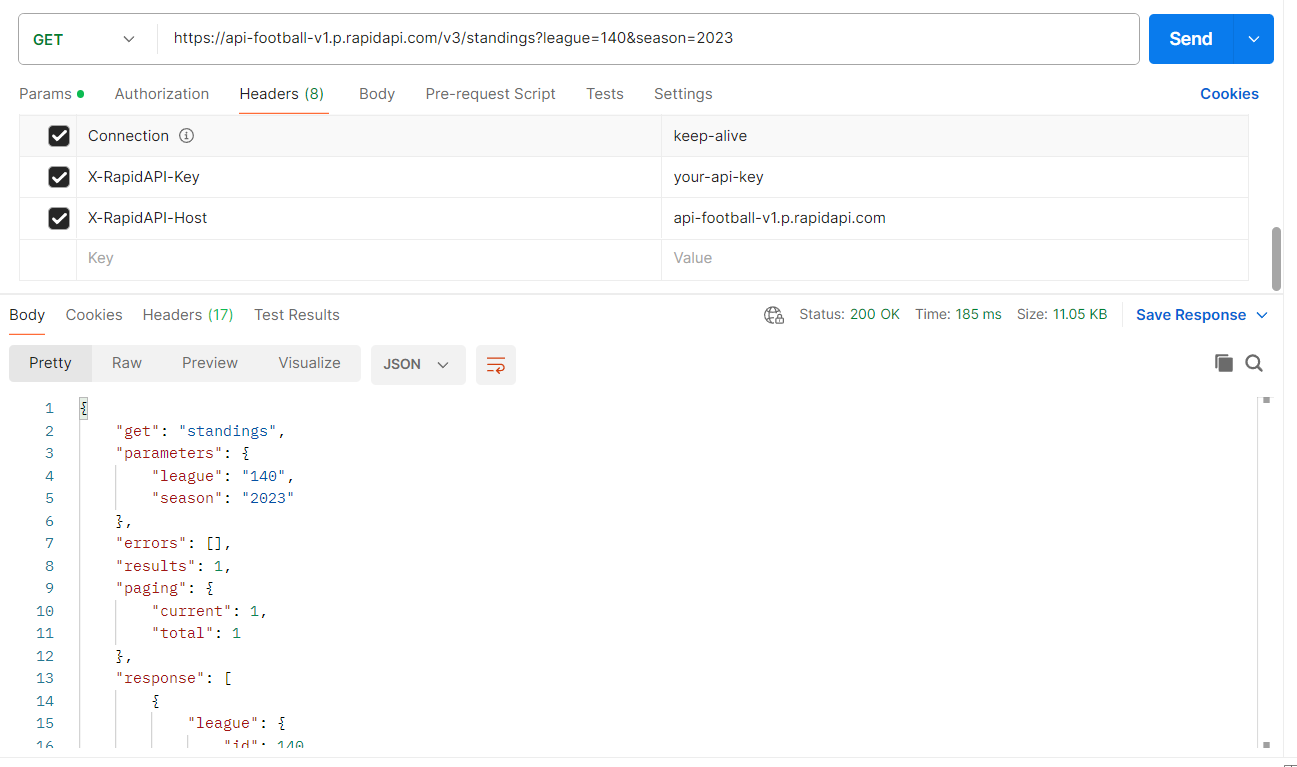
\includegraphics[width=1\linewidth]{img/ejemploPostman.png}
    \caption{Ejemplo de petición a API-FOOTBALL}
    \label{fig:enter-label}
\end{figure}

Como podemos ver se realiza una petición GET al \textit{endpoint} '/standings' para obtener una clasificación en concreto. Le pasamos como parámetros el identificador de liga 140(es el identificador de La Liga española) y la season 2023(año de la clasificación). Para que la petición tenga éxito tenemos que establecer en los headers el campo 'X-RapidAPI-Key' con la Api-key que da API-FOOTBALL al registrarse y el campo 'X-RapidAPI-Host' con el host correspondiente que en mi caso es 'api-football-v1.p.rapidapi.com'. Como podemos observas en el body observamos el resultado en JSON de la petición GET y el status de la petición que ha sido un 200 OK.
\subsection{Estructura de solicitudes y respuestas de la API en Flask}
La API diseñada en Flask contiene varios \textit{endpoints}. Algunos devuelven un JSON con la información del modelo de goles esperados o con la información de la tablas de los puntos esperados. En cambio, otros devuelven imágenes generadas en Python utilizando los datos de StatsBomb.\\
En la figura C.2 muestro un ejemplo de petición a la API creada en Flask:

\begin{figure}[H]
    \centering
    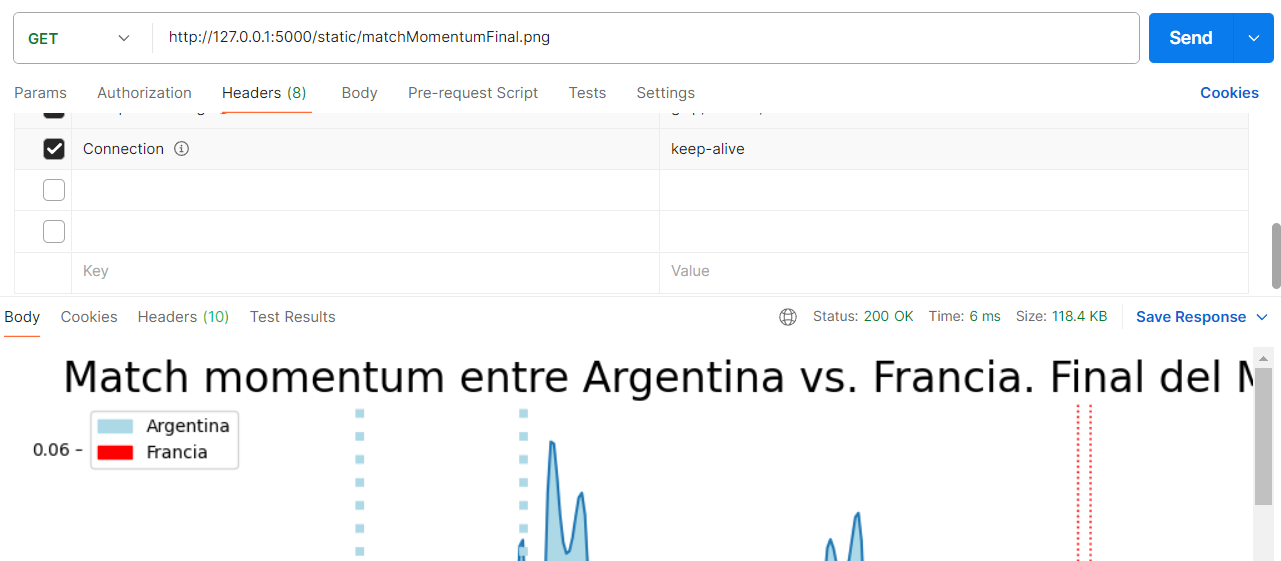
\includegraphics[width=1\linewidth]{img/ejemploPostman2.png}
    \caption{Ejemplo de petición a la API de Flask}
    \label{fig:enter-label}
\end{figure}

Como podemos ver en la imagen, se realiza una petición a un \textit{endpoint} que devuelve una imagen. En este caso basta con hacer la petición al \textit{endpoint} correcto sin utilizar una Api-key.

\subsection{Manejo de datos en memoria}
Los datos recibidos de la API se almacenan temporalmente en la memoria del cliente \textit{(front-end)} para su visualización y en el servidor (\textit{back-end}) para el procesamiento de predicciones y seguimiento de jugadores con ImageAI. \\
Cuando se realiza una petición a la API-FOOTBALL desde el \textit{front-end} desarrollado en Angular, los datos recibidos se almacenan en memoria en el cliente. Esto permite que la aplicación web pueda mostrar rápidamente la información solicitada por el usuario sin necesidad de realizar repetidas consultas a la API. Los datos en memoria se gestionan mediante servicios de Angular que mantienen el estado de la aplicación. \\
Cuando se realiza una petición al \textit{back-end}, los datos también se manejan en memoria temporalmente. Además, los datos procesados, como gráficos e imágenes, se guardan en las carpetas 'static' y 'uploads'. La carpeta static almacena imágenes de los gráficos generados, mientras que la carpeta uploads se utiliza para almacenar los vídeos procesados. \\
En resumen, los datos de la API-FOOTBALL se almacenan temporalmente en la memoria del frontend Angular para una rápida visualización y se manejan en memoria en el \textit{back-end} Flask para el procesamiento de predicciones y vídeos, guardando los resultados en las carpetas 'static' y 'uploads'.

\section{Diseño procedimental}
En esta sección se describen los flujos de trabajo y procedimientos clave en FutboStats.

\subsection{Flujo de búsqueda de datos en API-FOOTBALL}
\begin{enumerate}
	\item El usuario ingresa los criterios de búsqueda (fecha, nombre del equipo, nombre de la liga).
	\item El \textit{front-end} envía una solicitud a API-FOOTBALL a través de los servicios de Angular.
        \item La API-FOOTBALL devuelve los datos a Angular.
        \item Angular procesa los datos y los envía a la vista.
        \item Se muestran los resultados al usuario.
\end{enumerate}

\begin{figure}[H]
    \centering
    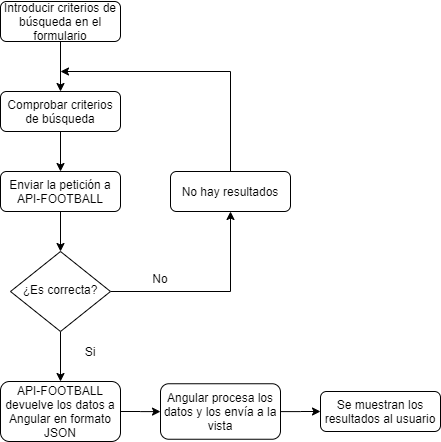
\includegraphics[width=0.7\linewidth]{img/flujo1.png}
    \caption{Diagrama de flujo de obtención de datos a API-FOOTBALL}
    \label{fig:enter-label}
\end{figure}


\subsection{Proceso de autenticación}
\begin{enumerate}
	\item El usuario selecciona la opción de iniciar sesión.
	\item El \textit{front-end} redirige al usuario al proveedor de autenticación (Google).
        \item El usuario se autentica y se redirige de vuelta al \textit{front-end} con un token.
        \item El \textit{front-end} valida el token utilizando las bibliotecas de autenticación de Google.
        \item Se crea una sesión para el usuario.
        \item El usuario puede acceder a las funcionalidades protegidas de la aplicación.
\end{enumerate}

\begin{figure}[H]
    \centering
    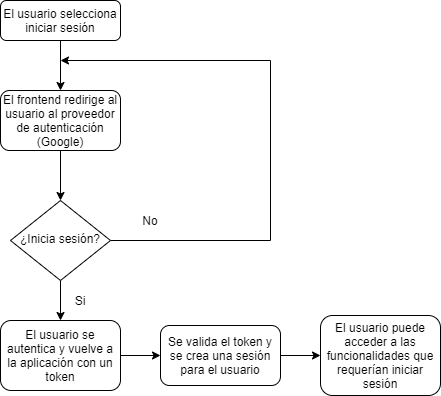
\includegraphics[width=0.7\linewidth]{img/flujo2.png}
    \caption{Diagrama de flujo de inicio de sesión en FutboStats}
    \label{fig:enter-label}
\end{figure} 

\subsection{Flujo de predicciones}
\begin{enumerate}
	\item El usuario inicia sesión y accede a la sección de predicciones.
	\item El \textit{front-end} envía una solicitud al \textit{back-end} para obtener los datos de las predicciones(goles esperados, puntos esperados, gráficos del mundial).
        \item El \textit{back-end} realiza cálculos utilizando los datos de la librería StatsBombPy.
        \item El \textit{back-end} devuelve los resultados del modelo al \textit{front-end}.
        \item El \textit{front-end} muestra las predicciones al usuario en forma de gráficos y tablas.
\end{enumerate}
\begin{figure}[H]
    \centering
    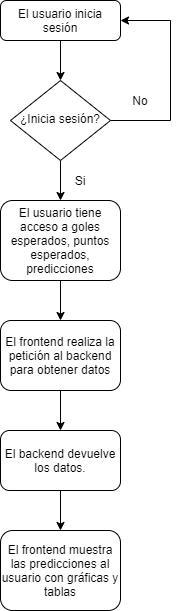
\includegraphics[width=0.3\linewidth]{img/flujo3.png}
    \caption{Diagrama de flujo de obtención de datos en la API de Flask}
    \label{fig:enter-label}
\end{figure}

\subsection{Procesamiento de vídeos para tracking}
\begin{enumerate}
    \item El usuario inicia sesión y accede a la sección de SportsAI.
    \item El usuario sube un vídeo a la aplicación.
    \item El \textit{front-end} envía el vídeo al \textit{back-end}.
    \item El \textit{back-end} procesa el vídeo utilizando el modelo de \textit{tracking} de ImageAI.
    \item El \textit{back-end} genera un vídeo procesado con el \textit{tracking} aplicado.
    \item El \textit{back-end} envía el vídeo procesado al \textit{front-end}.
    \item El \textit{front-end} muestra el vídeo procesado al usuario. 
\end{enumerate}

\begin{figure}[H]
    \centering
    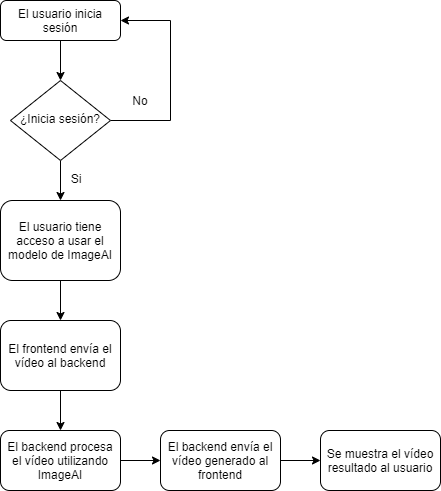
\includegraphics[width=0.7\linewidth]{img/flujo4.png}
    \caption{Diagrama de flujo de uso de ImageAI}
    \label{fig:enter-label}
\end{figure}

\section{Diseño arquitectónico}
FutboStats utiliza una arquitectura cliente-servidor porque divide claramente las responsabilidades entre el \textit{front-end} y el \textit{back-end}, se comunican a través de peticiones HTTP, y facilita la interacción con servicios externos, el procesamiento de datos y la independencia de plataforma \cite{web:clienteServidor}. El \textit{front-end} está desarrollado en Angular y el \textit{back-end} en Flask. La aplicación interactúa con la API-FOOTBALL para obtener los datos necesarios.
\subsection{Descripción general de la arquitectura}
La arquitectura de FutboStats se divide en dos capas principales: el \textit{front-end} y el \textit{back-end}. 
Tiene las siguientes características de una arquitectura cliente-servidor:
\begin{itemize}
    \item \textbf{Separación de responsabilidades:} en FutboStats, el \textit{front-end} (cliente) está desarrollado en Angular y se encarga de la interfaz de usuario y los servicios que hacen las peticiones a API-FOOTBALL, gestionando las interacciones del usuario y la presentación de los datos. El \textit{back-end} (servidor), desarrollado en Flask, maneja la lógica de negocio y el procesamiento de los datos, gráficos, imágenes y vídeos.
    \item \textbf{Comunicación a través de HTTP:} la arquitectura cliente-servidor implica que el cliente y el servidor se comuniquen a través de peticiones HTTP. En FutboStats, el frontend realiza peticiones HTTP al backend para obtener datos de predicciones, modelos, gráficos y este responde con la información pedida.
    \item \textbf{Independencia de plataforma:} esta arquitectura permite que el cliente y el servidor se ejecuten en plataformas diferentes. El \textit{front-end} puede ser accedido desde cualquier navegador web (desplegado en Netlify), mientras que el \textit{back-end} puede estar alojado en un servidor remoto(desplegado en Render). Esta separación facilita la escalabilidad y el mantenimiento de la aplicación.
    \item \textbf{Procesamiento de datos en el servidor:} el procesamiento de predicciones, generación de gráficos y el tracking de vídeos, se realizan en el \textit{back-end}. Esto descarga al cliente de tareas intensivas en recursos y permite una mayor eficiencia y seguridad en el manejo de datos.
\end{itemize}
En la figura C.7 se muestra la arquitectura cliente-servidor.
\begin{figure}[H]
    \centering
    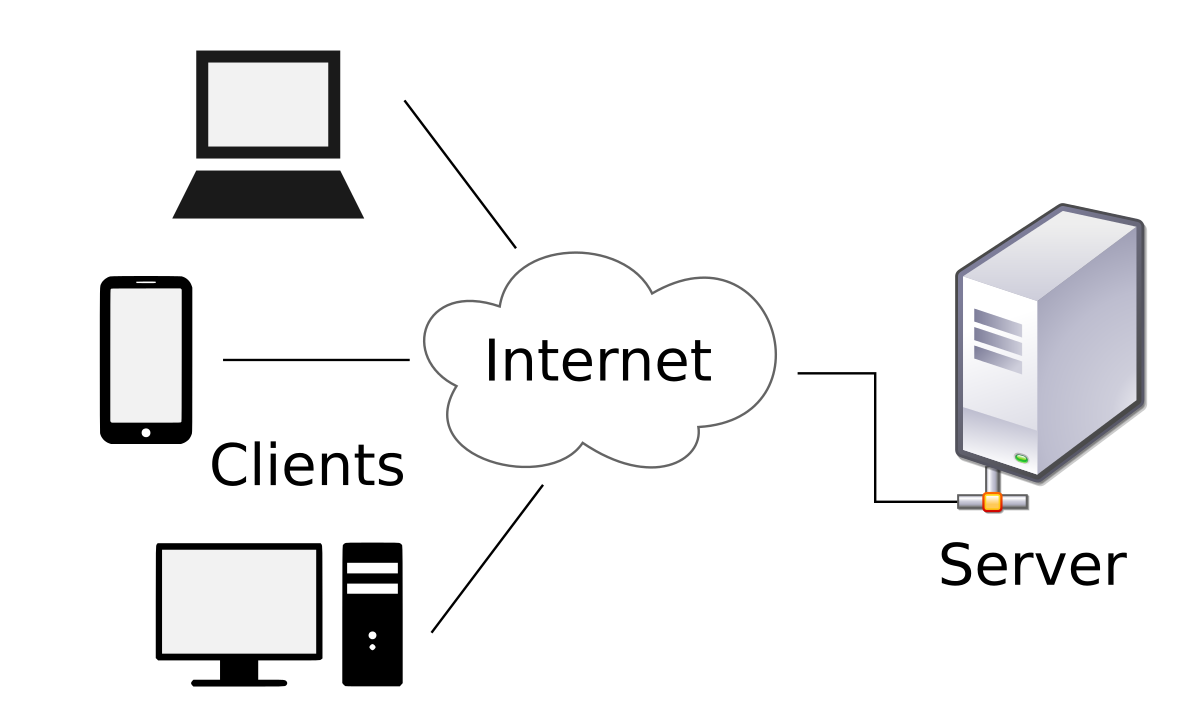
\includegraphics[width=0.7\linewidth]{img/cliente-servidor.png}
    \caption{Arquitectura cliente-servidor \cite{web:clienteServidor2}}
    \label{fig:enter-label}
\end{figure}

\subsection{Componentes principales}
\textbf{Frontend (Angular):}
\begin{itemize}
    \item Componente de búsqueda: permite a los usuarios buscar partidos, equipos y clasificaciones mediante la interacción del usuario.
    \item Componente de visualización: muestra los resultados de búsqueda y estadísticas mediante tablas y tarjetas.
    \item Componente de autenticación: gestiona el inicio de sesión de los usuarios.
    \item Servicios que manejan las peticiones a API-FOOTBALL.
\end{itemize}
\textbf{Backend (Flask):}
\begin{itemize}
    \item Módulo de predicciones: calcula las predicciones de puntos esperados y goles esperados.
    \item Generación de gráficos: se generan gráficos con los datos de StatsBombPy que son guardados en la carpeta 'static'.
    \item Módulo de procesamiento de videos: procesa los vídeos utilizando ImageAI.
\end{itemize}

\section{Diseño de interfaces}
En el diseño de la interfaz se han realizado varios prototipos inicialmente utilizando la aplicación \textit{JustInMind}. Estos primeros prototipos sirvieron para definir la paleta de colores que iba a usar la aplicación (verde, blanco y negro) y la distribución de las opciones del menú. \\
Las siguientes figuras muestran algunos prototipos que fueron desarrollados con \textit{JustInMind}:

\begin{figure}[H]
    \centering
    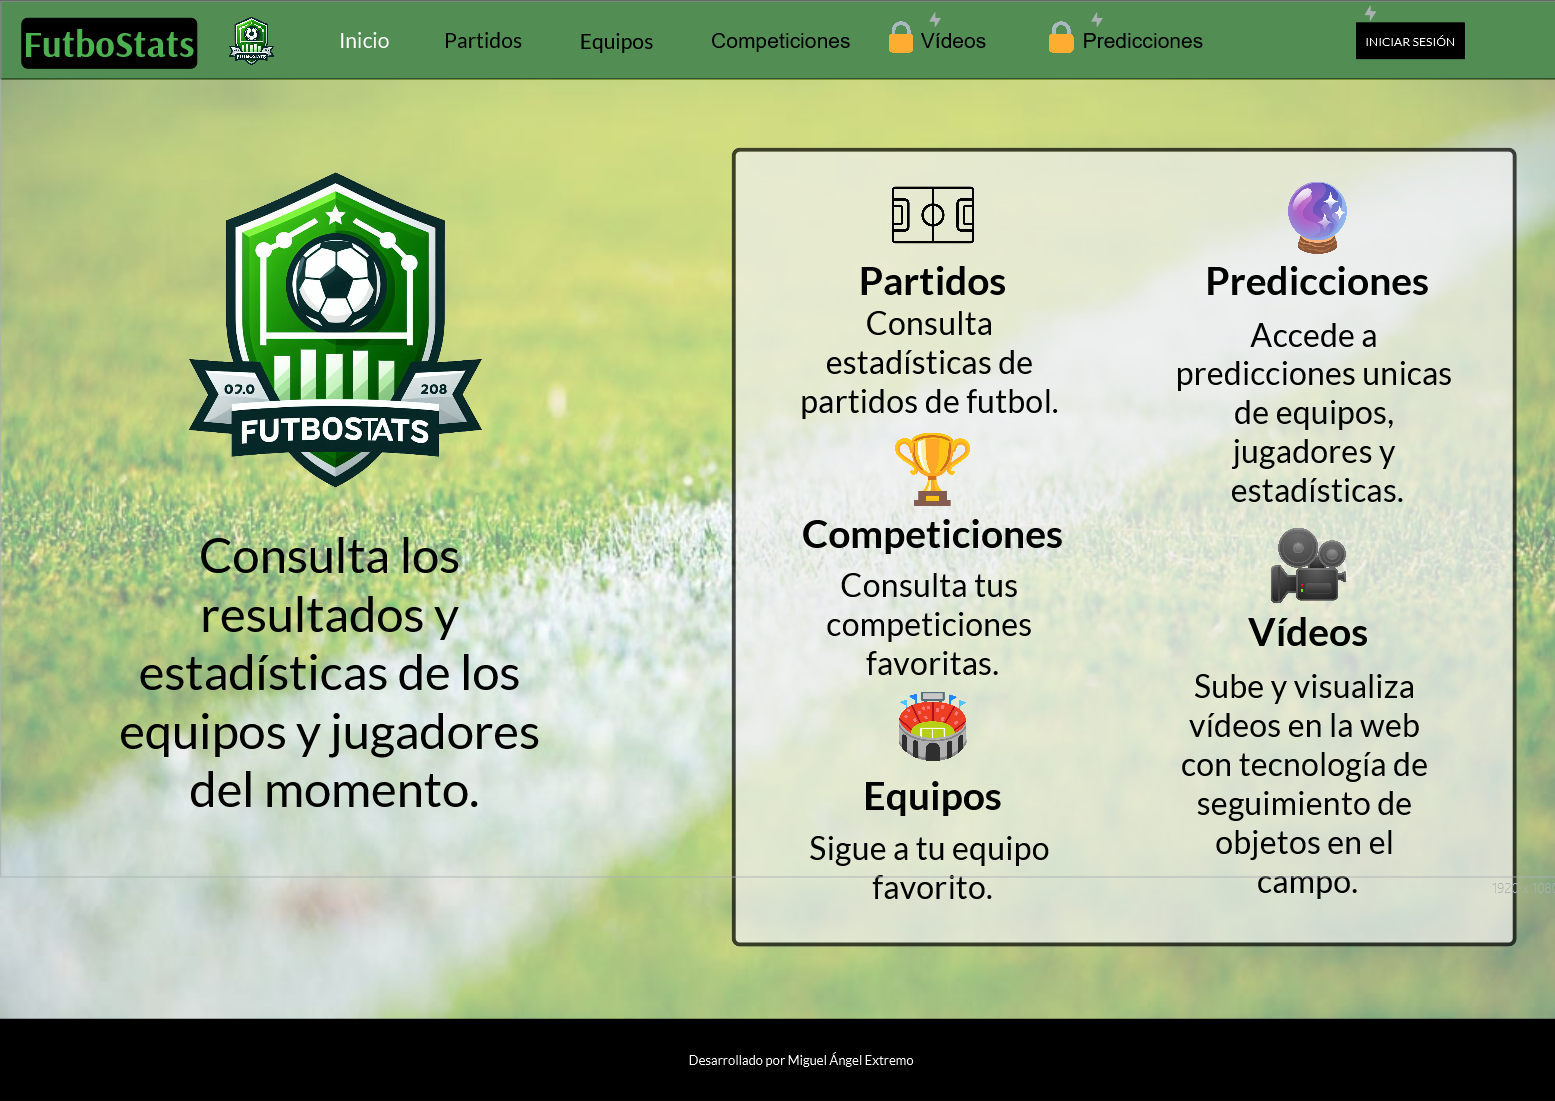
\includegraphics[width=0.7\linewidth]{img/prototipo.png}
    \caption{Prototipo de Inicio}
    \label{fig:enter-label}
\end{figure}

\begin{figure}[H]
    \centering
    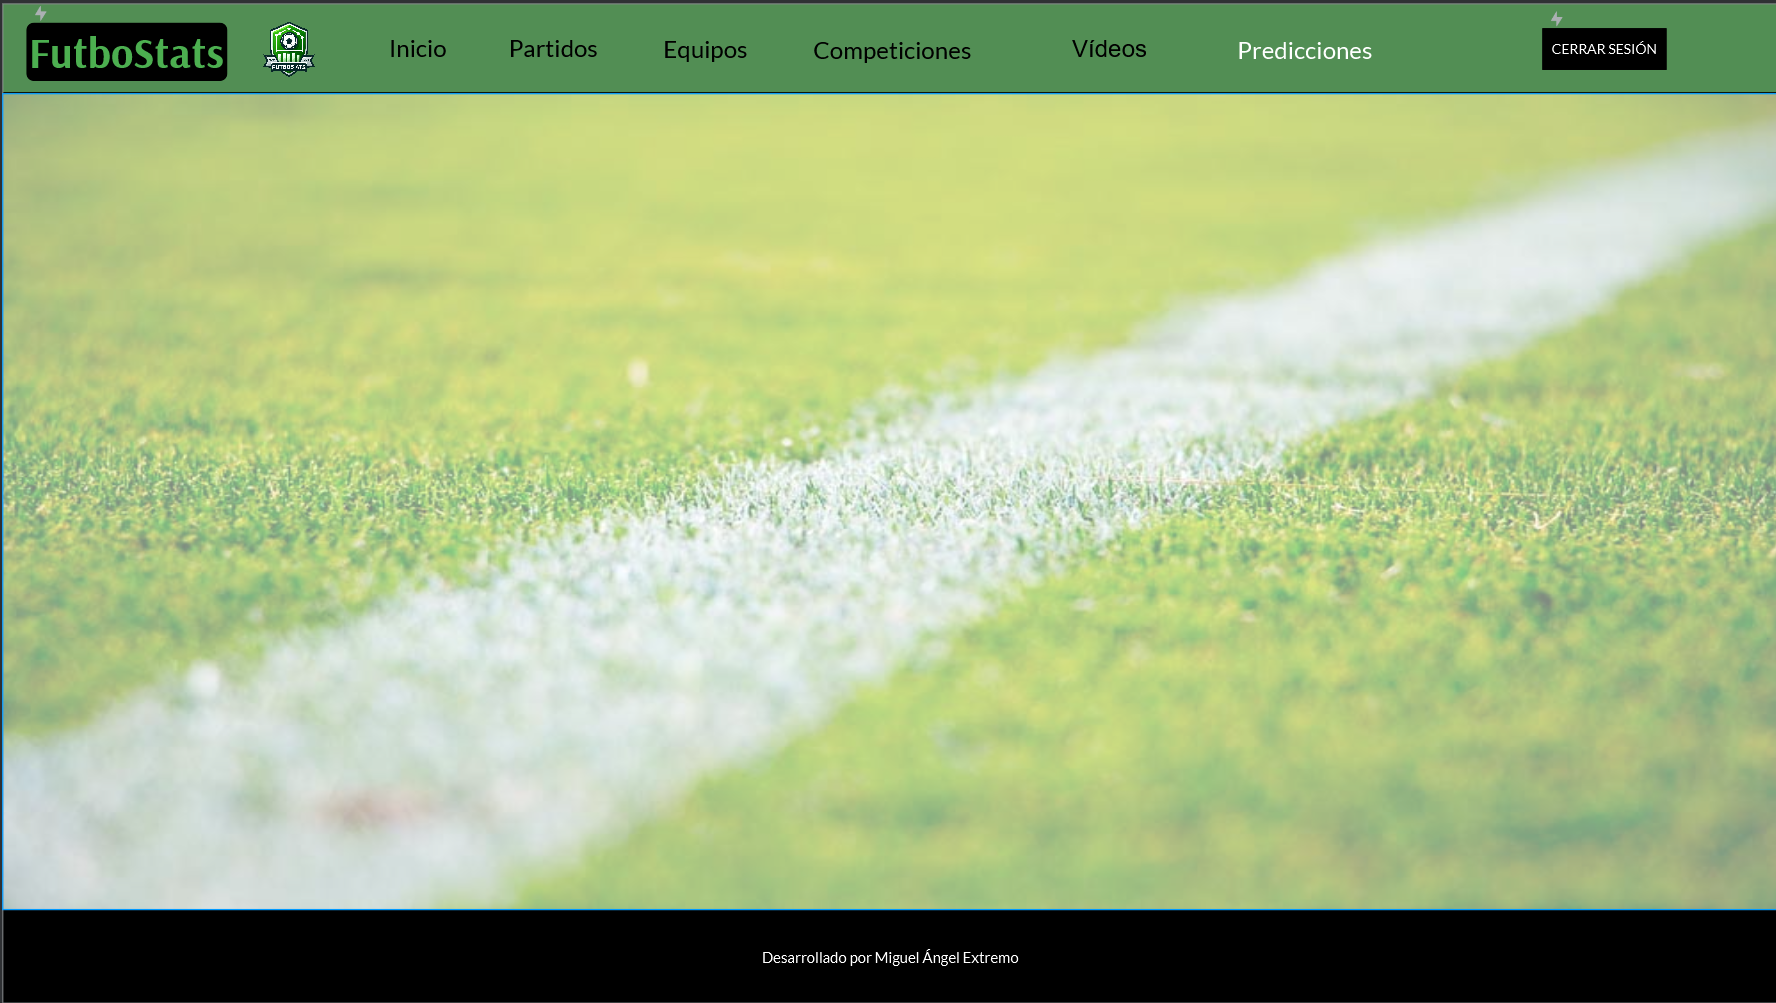
\includegraphics[width=0.7\linewidth]{img/prototipo3.png}
    \caption{Prototipo general con header, body y footer}
    \label{fig:enter-label}
\end{figure}

\begin{figure}[H]
    \centering
    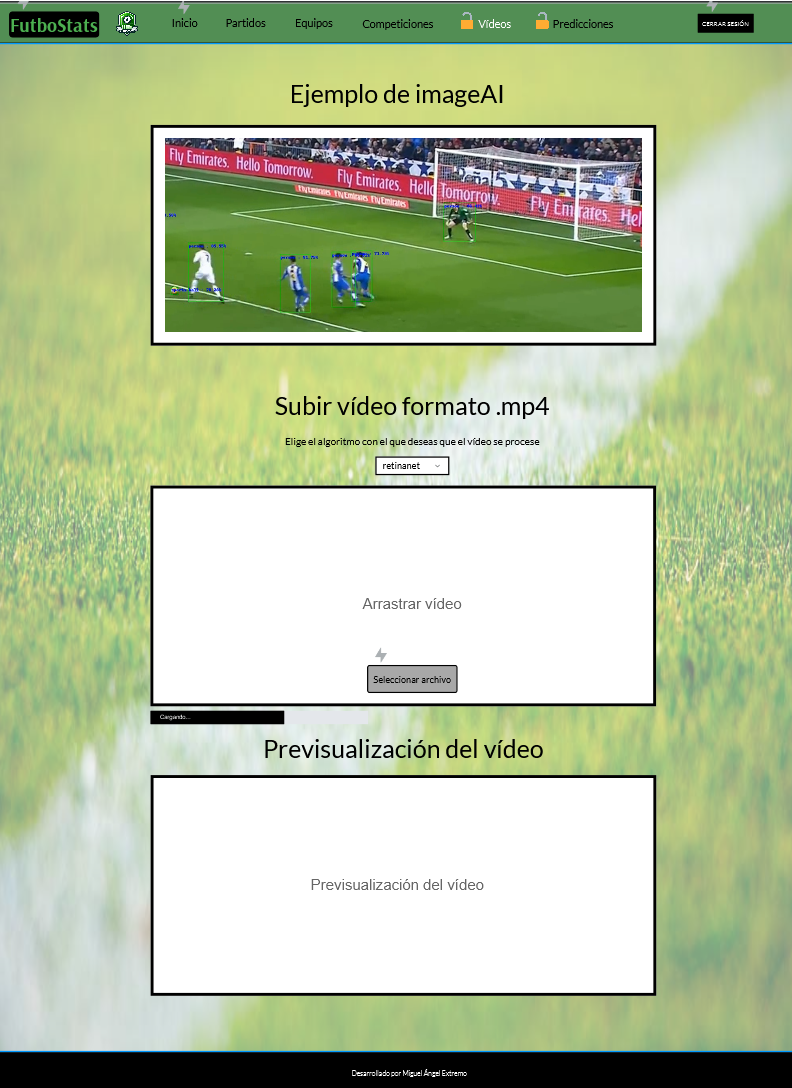
\includegraphics[width=0.7\linewidth]{img/prototipo2.png}
    \caption{Prototipo de la vista de ImageAI}
    \label{fig:enter-label}
\end{figure}


\apendice{Documentación técnica de programación}

\section{Introducción}

\section{Estructura de directorios}

\section{Manual del programador}

\section{Compilación, instalación y ejecución del proyecto}

\section{Pruebas del sistema}

\apendice{Documentación de usuario}

\section{Introducción}
En este apéndice se detallan los requerimientos de la aplicación y las indicaciones sobre cómo usarla correctamente. El manual de usuario aquí descrito también se aporta en formato vídeo para que se pueda ver de una forma dinámica como funciona la aplicación en tiempo real.

\section{Requisitos de usuarios}
Los requisitos para poder hacer uso de la aplicación son:
\begin{itemize}
    \item Tener acceso a internet estable para poder utilizar la aplicación.
    \item Tener un navegador web actualizado (Google Chrome, Mozilla Firefox, Microsoft Edge, Safari).
    \item Contar con un dispositivo móvil o un ordenador (portátil o de sobremesa). 
    \item Tener una cuenta de Google para iniciar sesión y acceder así a las funcionalidades protegidas de la aplicación.
\end{itemize}

\section{Instalación}
Para usar la aplicación FutboStats solamente es necesario que el usuario tenga un navegador web instalado en su dispositivo.
En el navegador web introducir la url de la web: \href{https://futbostats.netlify.app/}{https://futbostats.netlify.app/} 

\section{Manual del usuario}
En esta sección se describe el uso de las diferentes funcionalidades de la aplicación para que un usuario sin previo conocimiento de uso pueda utilizarla sin mayores problemas. Se aportarán imágenes ilustrativas con ejemplos reales de uso de la aplicación.

\subsection{Inicio}
El apartado de 'Inicio' de FutboStats supone una carta de presentación al usuario. Describe de forma resumida las funcionalidades, expone que la aplicación se puede utilizar en móvil, ya que, es responsiva y se dispone de pequeños tutoriales integrados en la aplicación que permiten enseñar al usuario como utilizar las ditintas funcionalidades haciendo el uso de la aplicación más fácil e intuitiva para el usuario.\\
Pasos para utilizar la página de 'Inicio':
\begin{enumerate}
    \item Pulsar en la opción del menú llamada 'Inicio'
    \item Consultar vídeos explicativos de las funcionalidades de la aplicación.
\end{enumerate}

\begin{figure}[H]
    \centering
    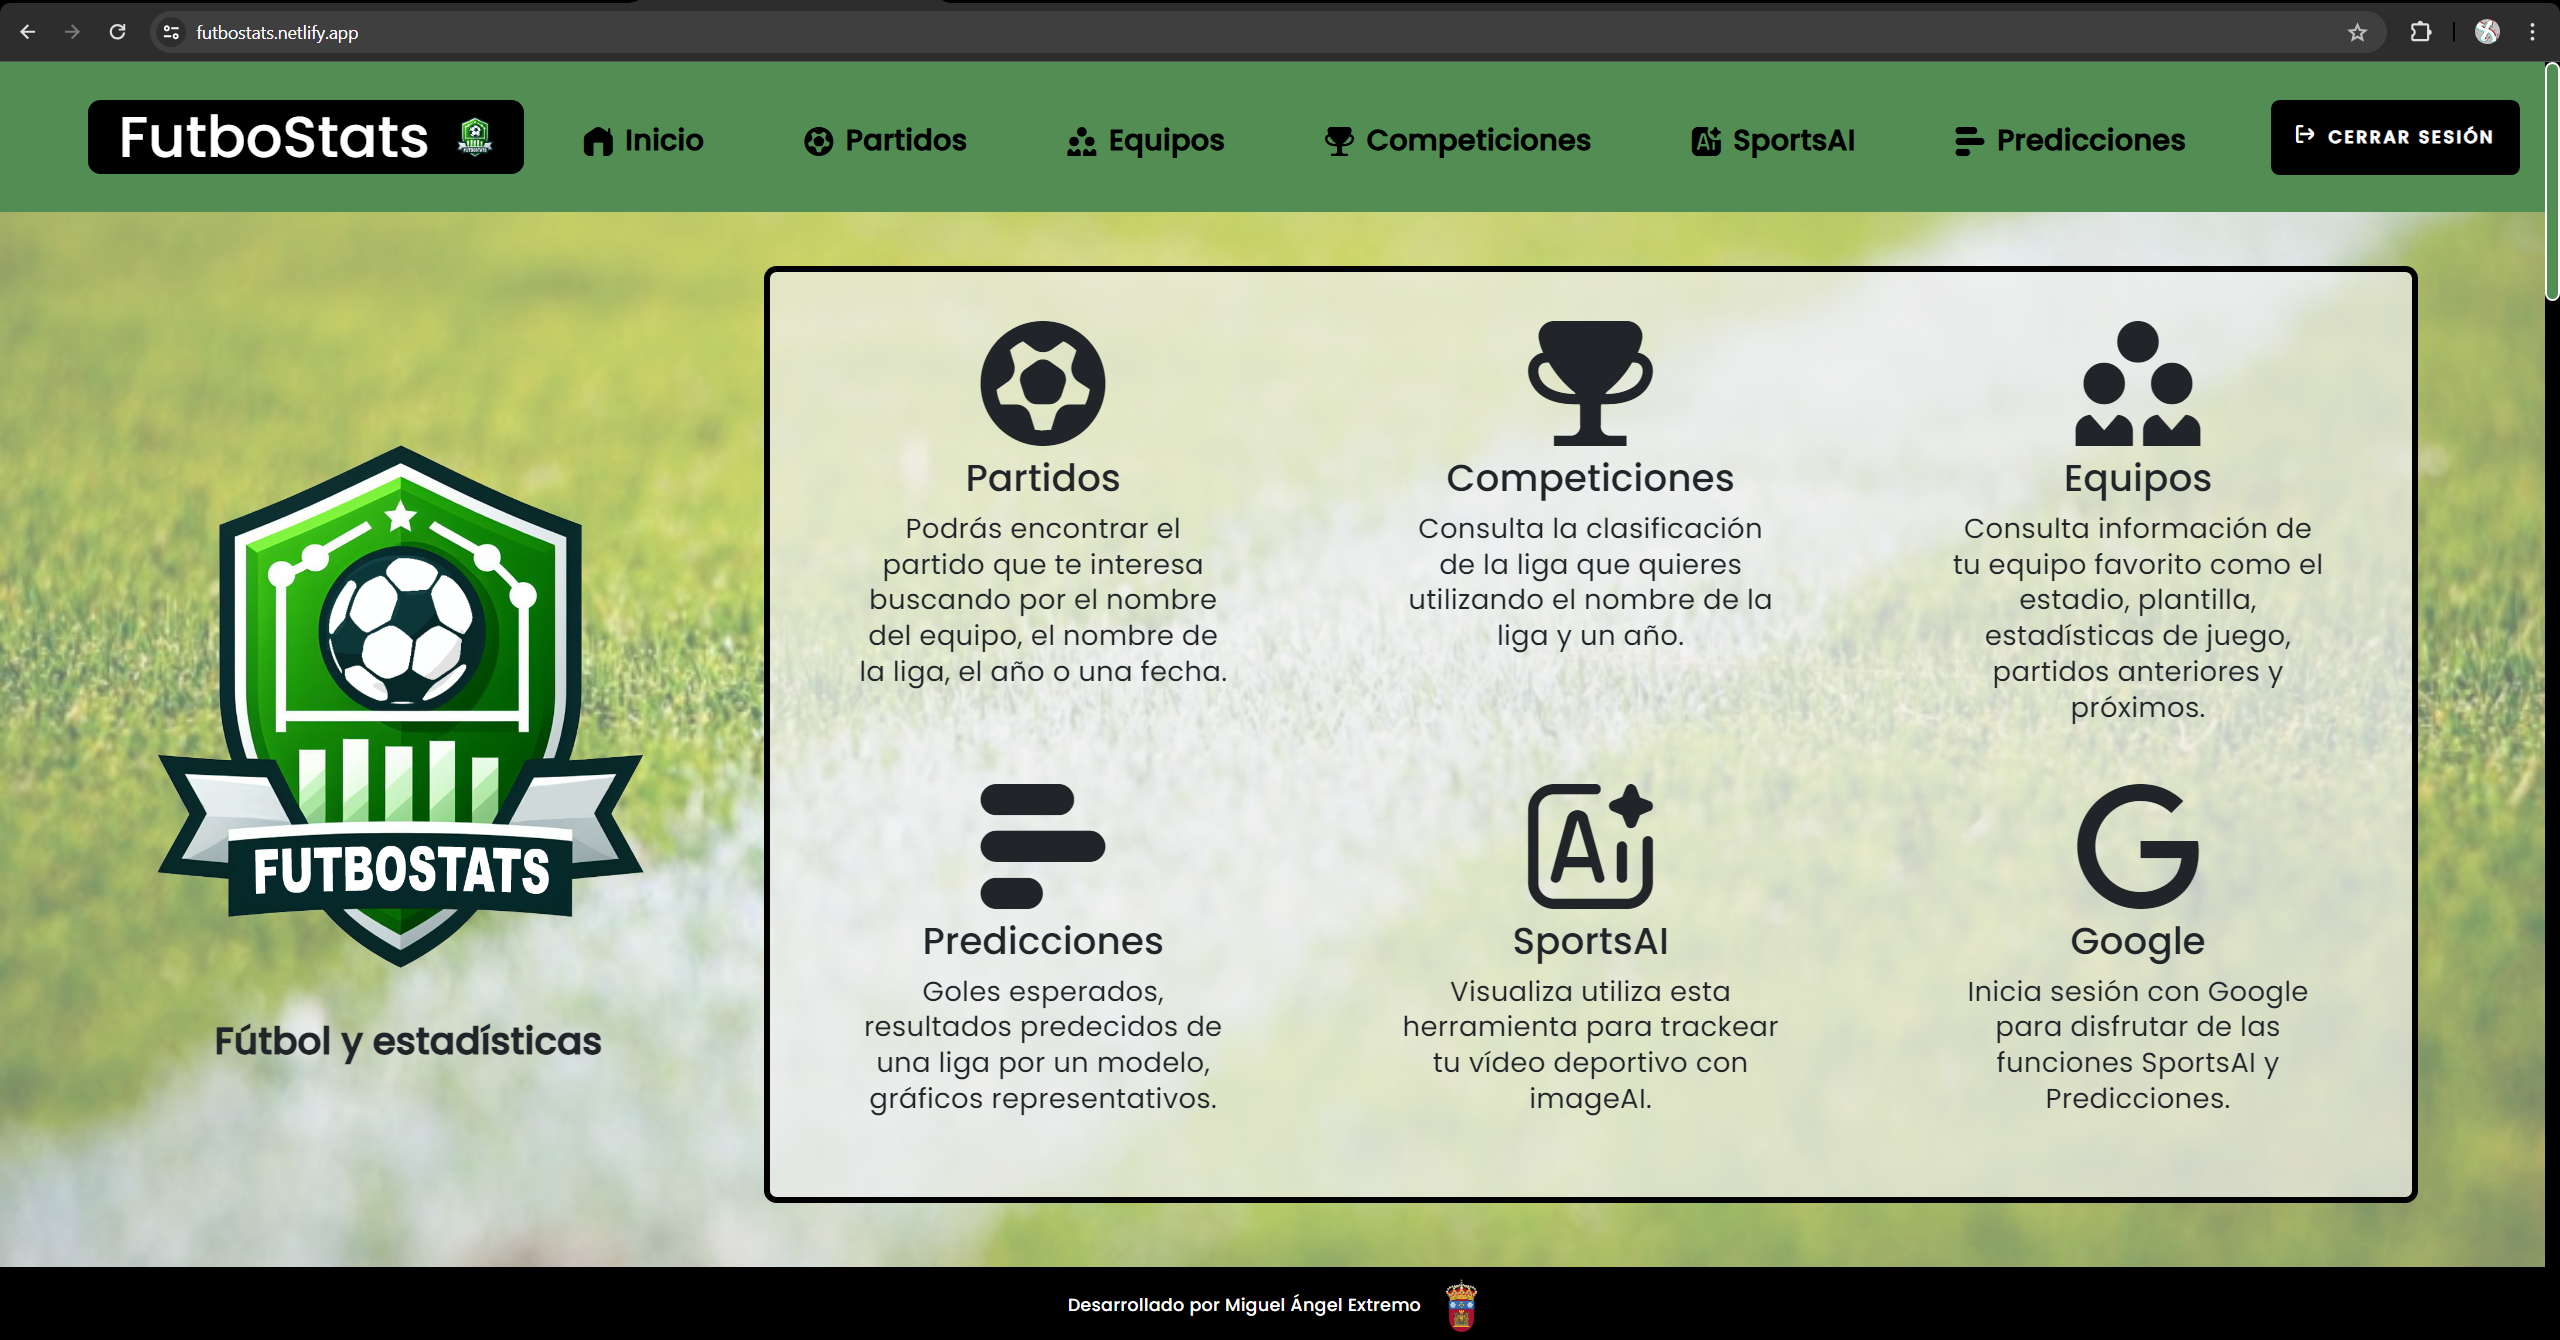
\includegraphics[width=1\linewidth]{img/inicio-UM.png}
    \caption{Inicio de FutboStats}
    \label{fig:enter-label}
\end{figure}

\begin{figure}[H]
    \centering
    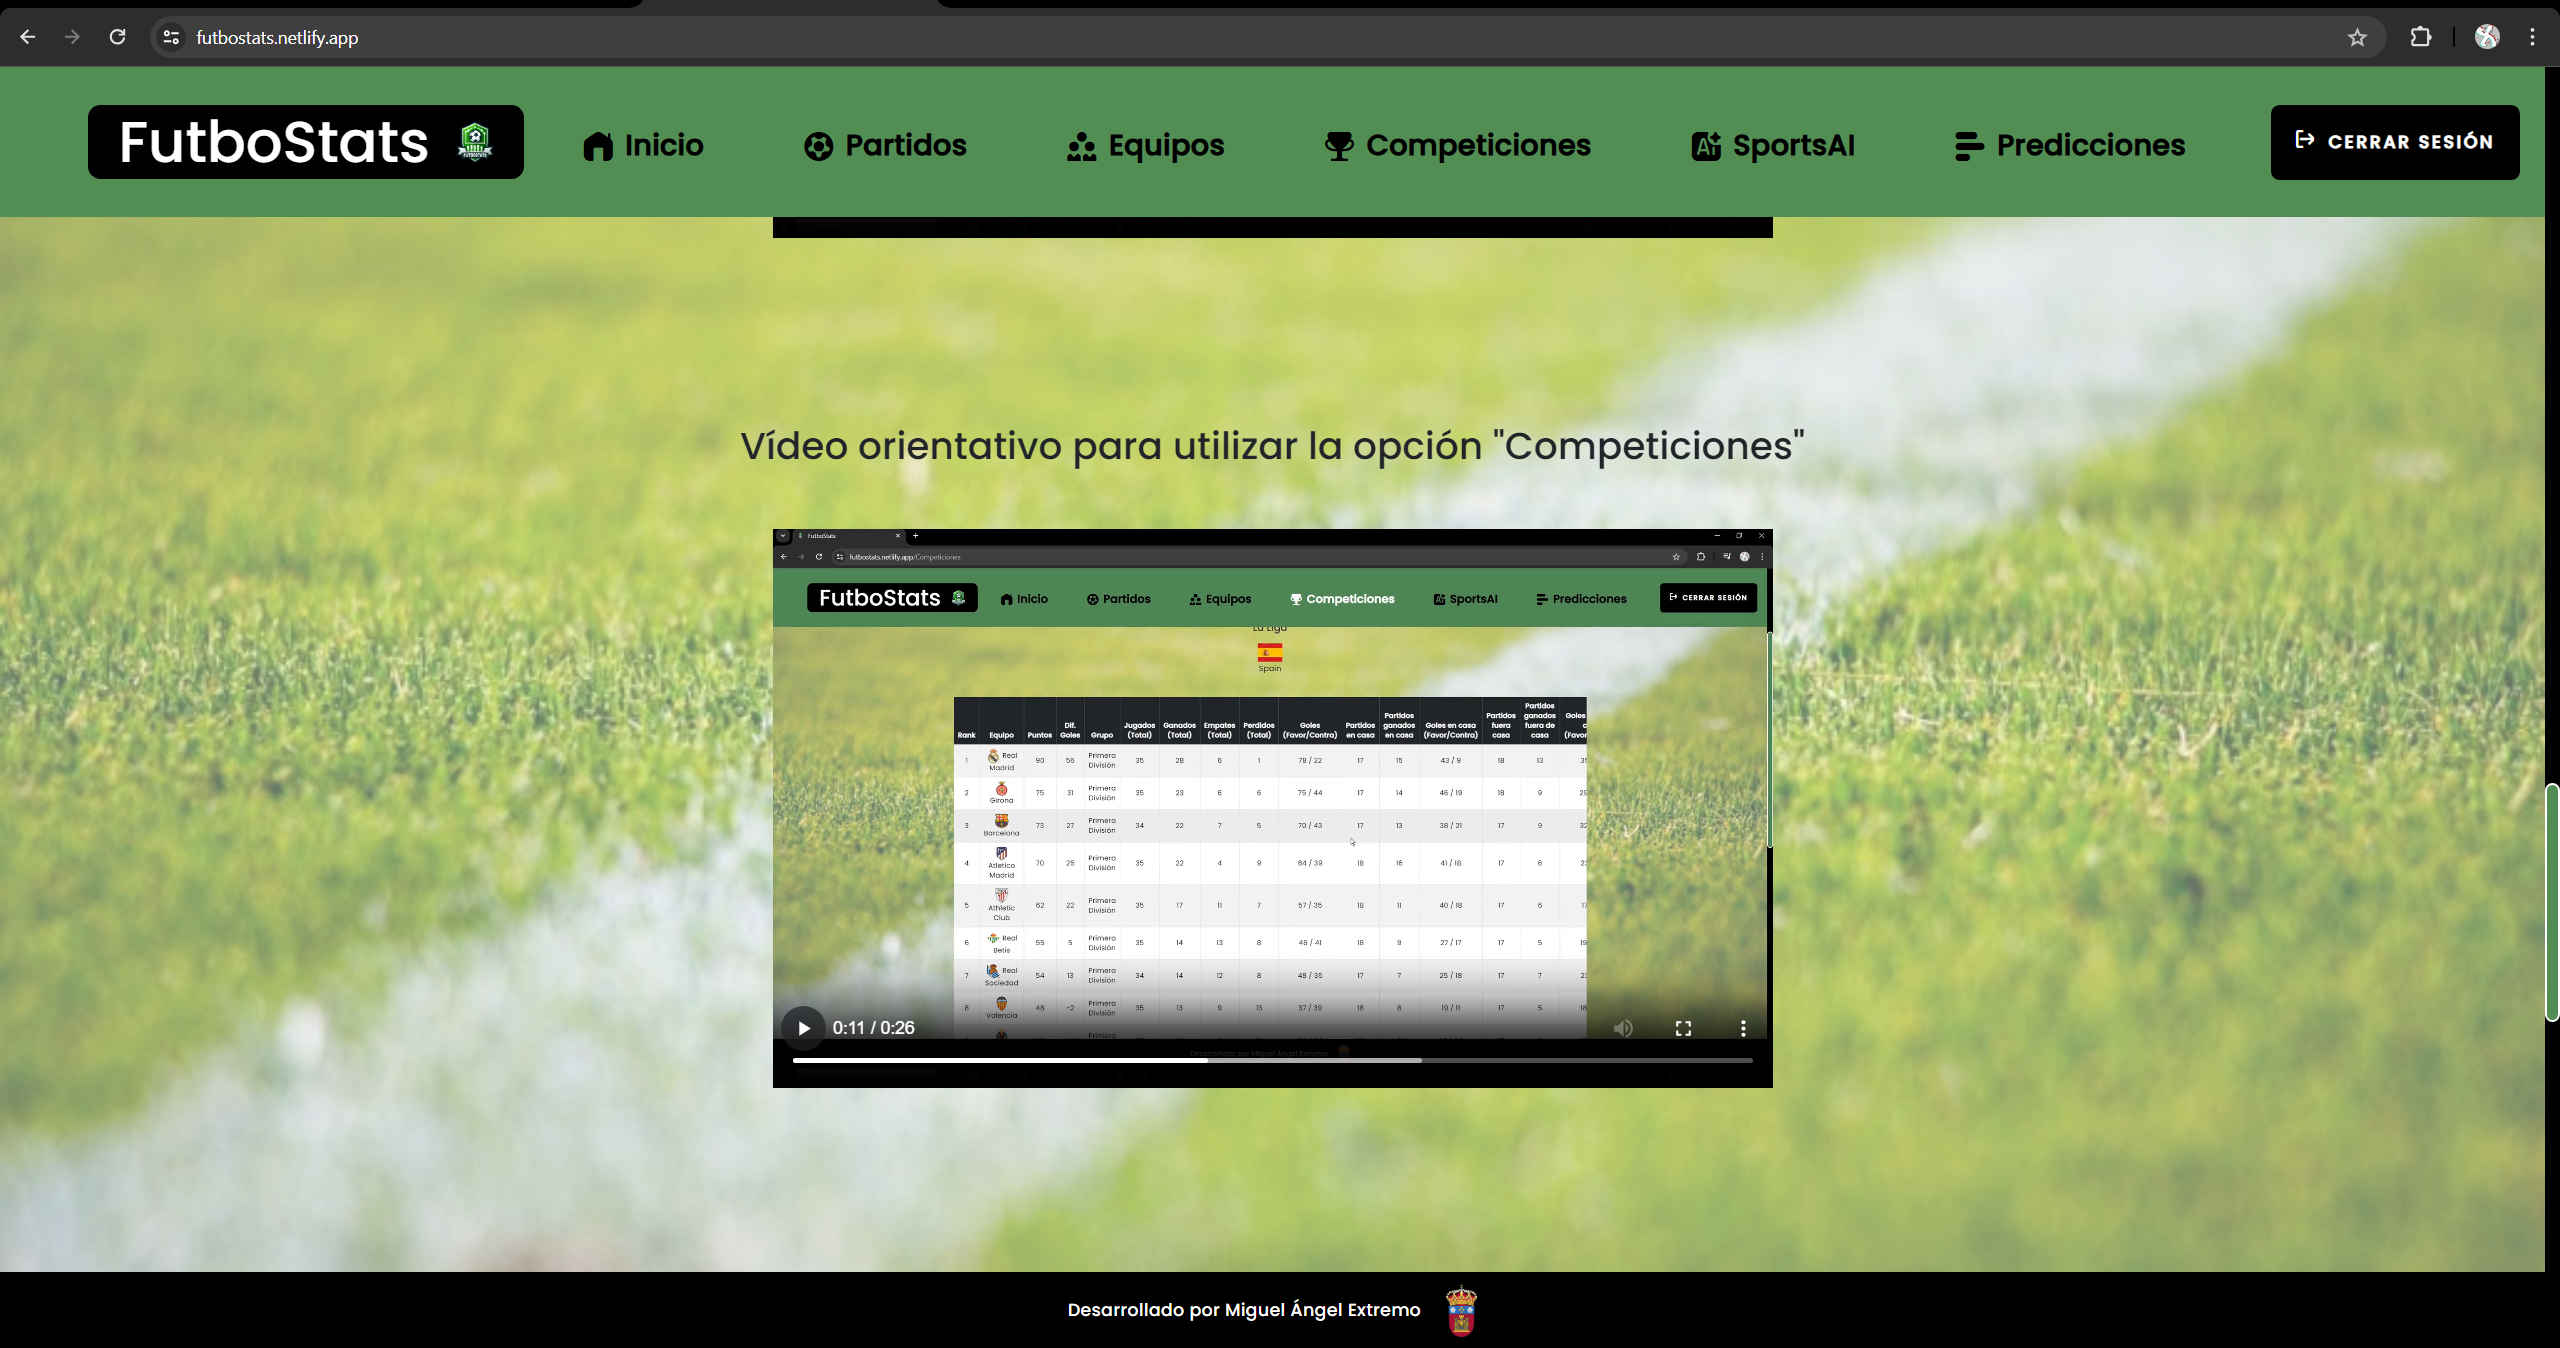
\includegraphics[width=1\linewidth]{img/inicio2-UM.png}
    \caption{Tutoriales en Inicio de FutboStats}
    \label{fig:enter-label}
\end{figure}

\subsection{Buscar partidos}
El apartado 'Partidos' de FutboStats proporciona al usuario una forma sencilla de buscar partidos introduciendo unos parámetros de búsqueda.\\
Para buscar partidos el usuario debe:
\begin{enumerate}
    \item Pulsar en el menú superior la opción 'Partidos'.
    \item Introducir el nombre de una liga. El sistema genera una lista de sugerencias al usuario a medida que este escribe.
    \item Introducir el nombre de un equipo.
    \item Introducir una fecha para filtrar los partidos.
    \item Para realizar la búsqueda de partidos es obligatorio introducir el nombre de la liga o el nombre del equipo.
    \item La fecha es un parámetro opcional para ofrecer un mayor filtrado.
    \item Por último, dar al botón buscar.
    \item El usuario visualiza los resultados de la búsqueda.
    \item En el caso de no haber partidos con esos filtros, se le informa al usuario mediante un mensaje.
\end{enumerate}

\begin{figure}[H]
    \centering
    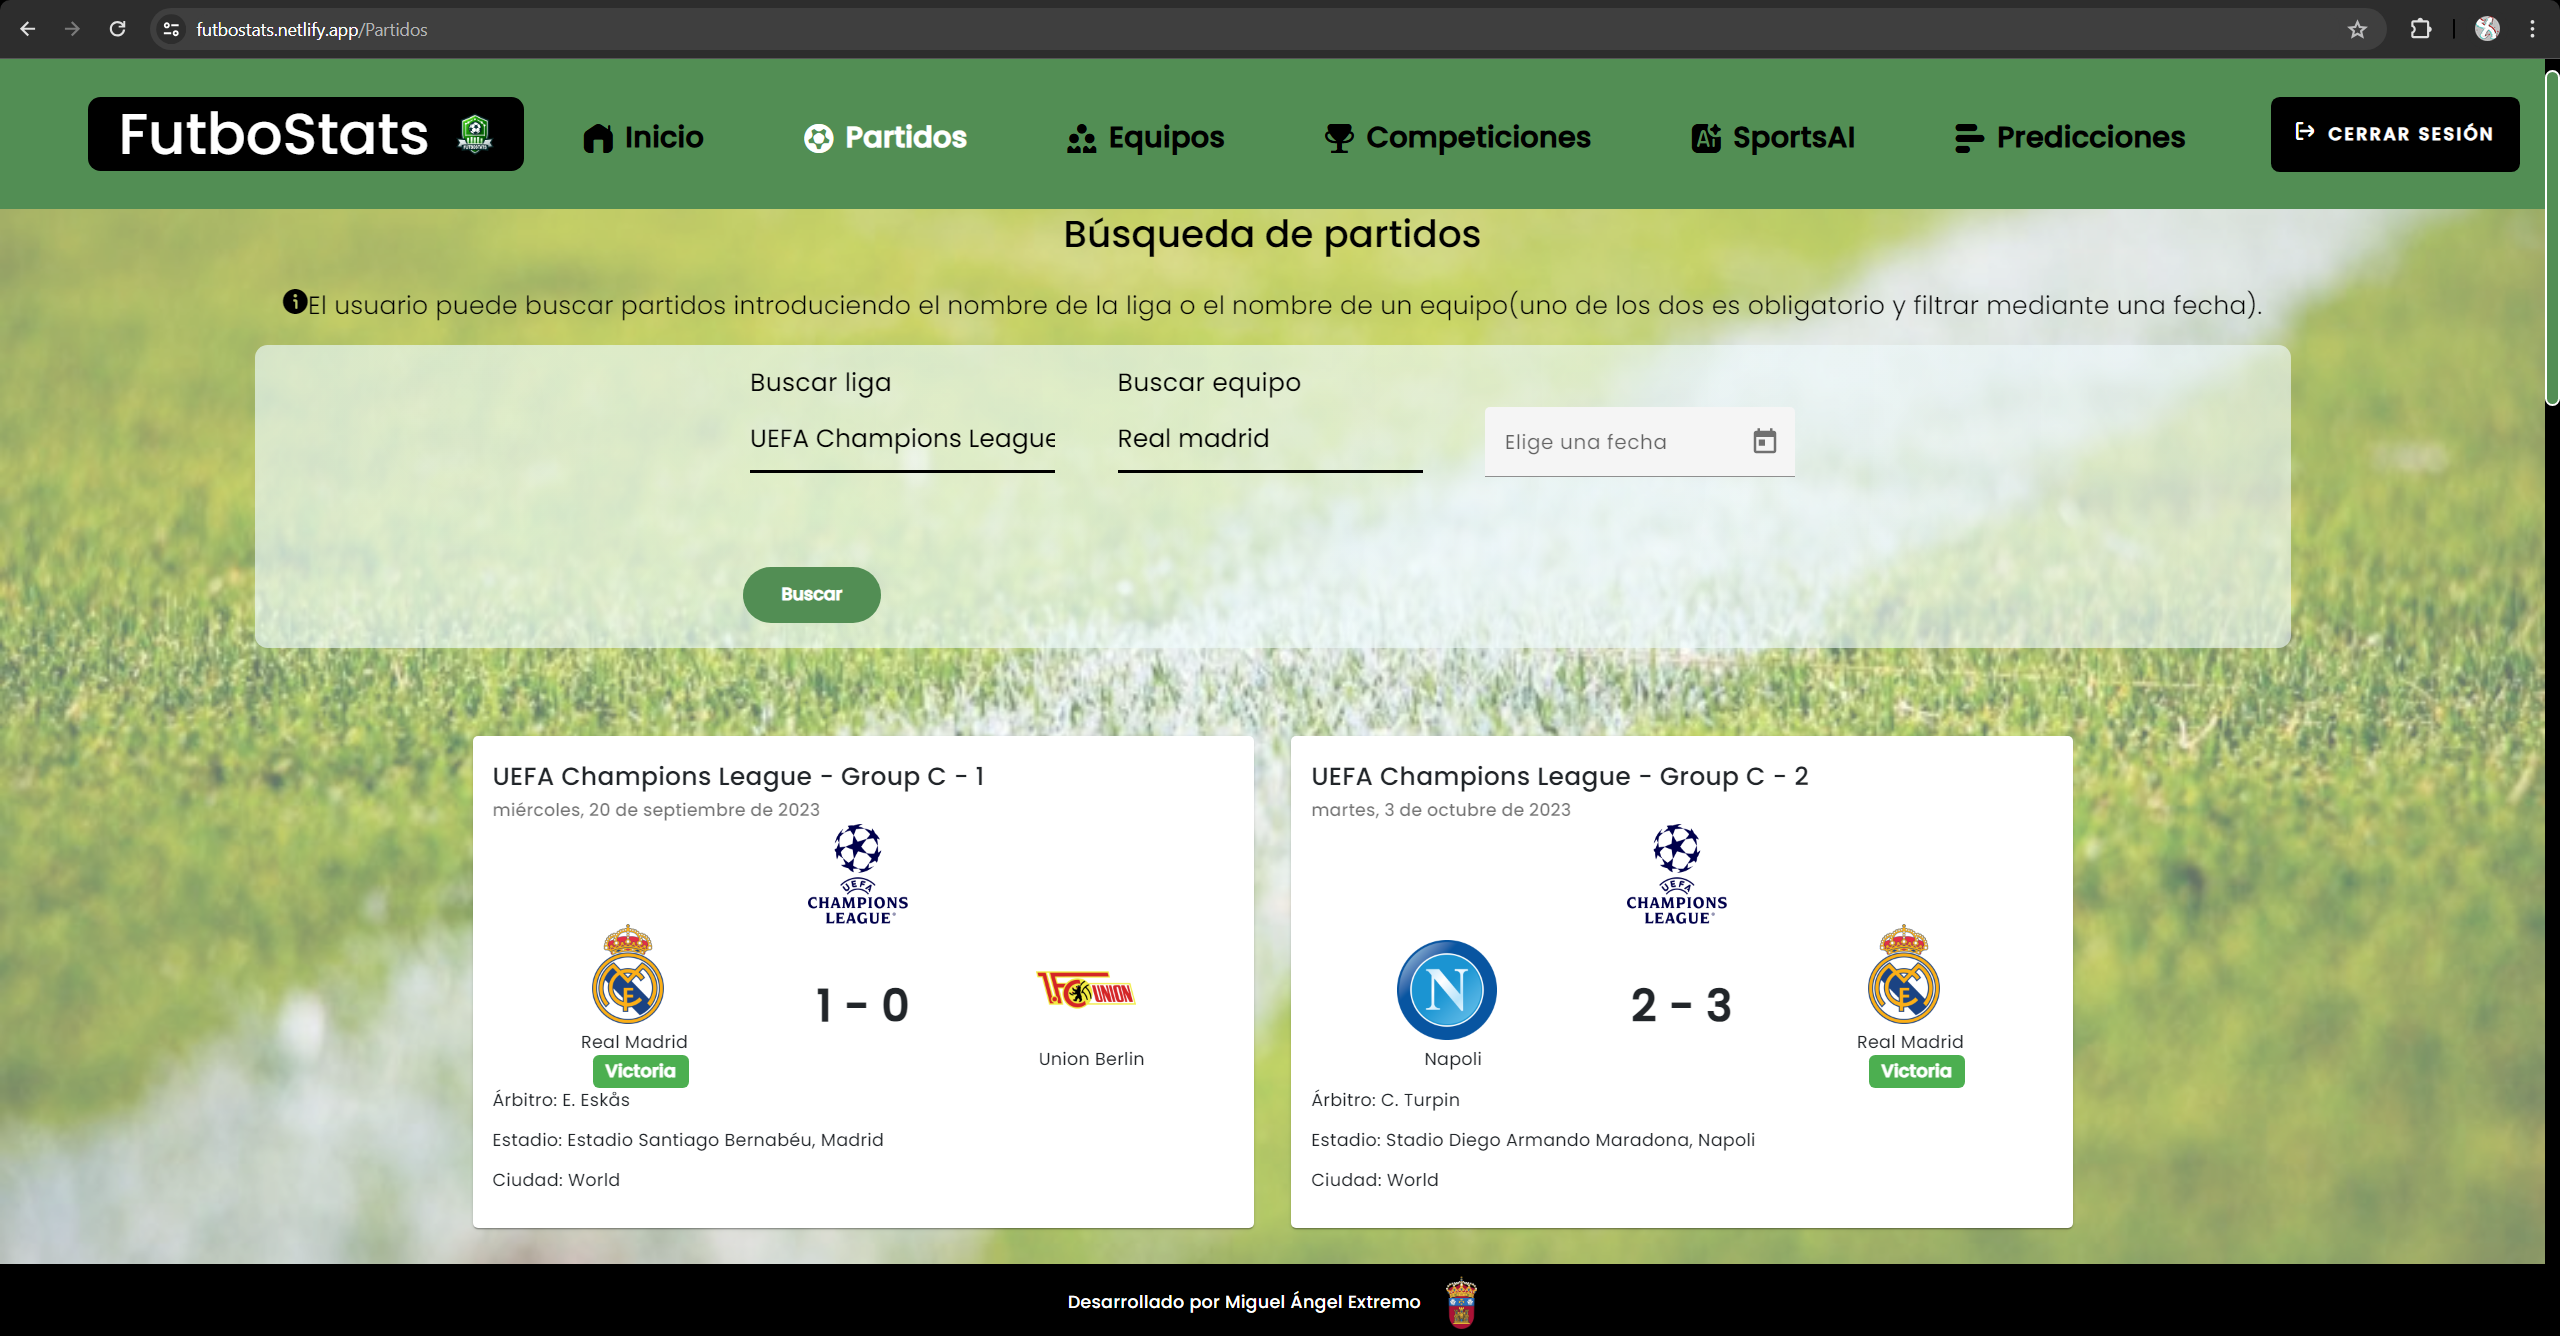
\includegraphics[width=1\linewidth]{img/partidos-UM.png}
    \caption{Búsqueda de partidos en FutboStats}
    \label{fig:enter-label}
\end{figure}

\begin{figure}[H]
    \centering
    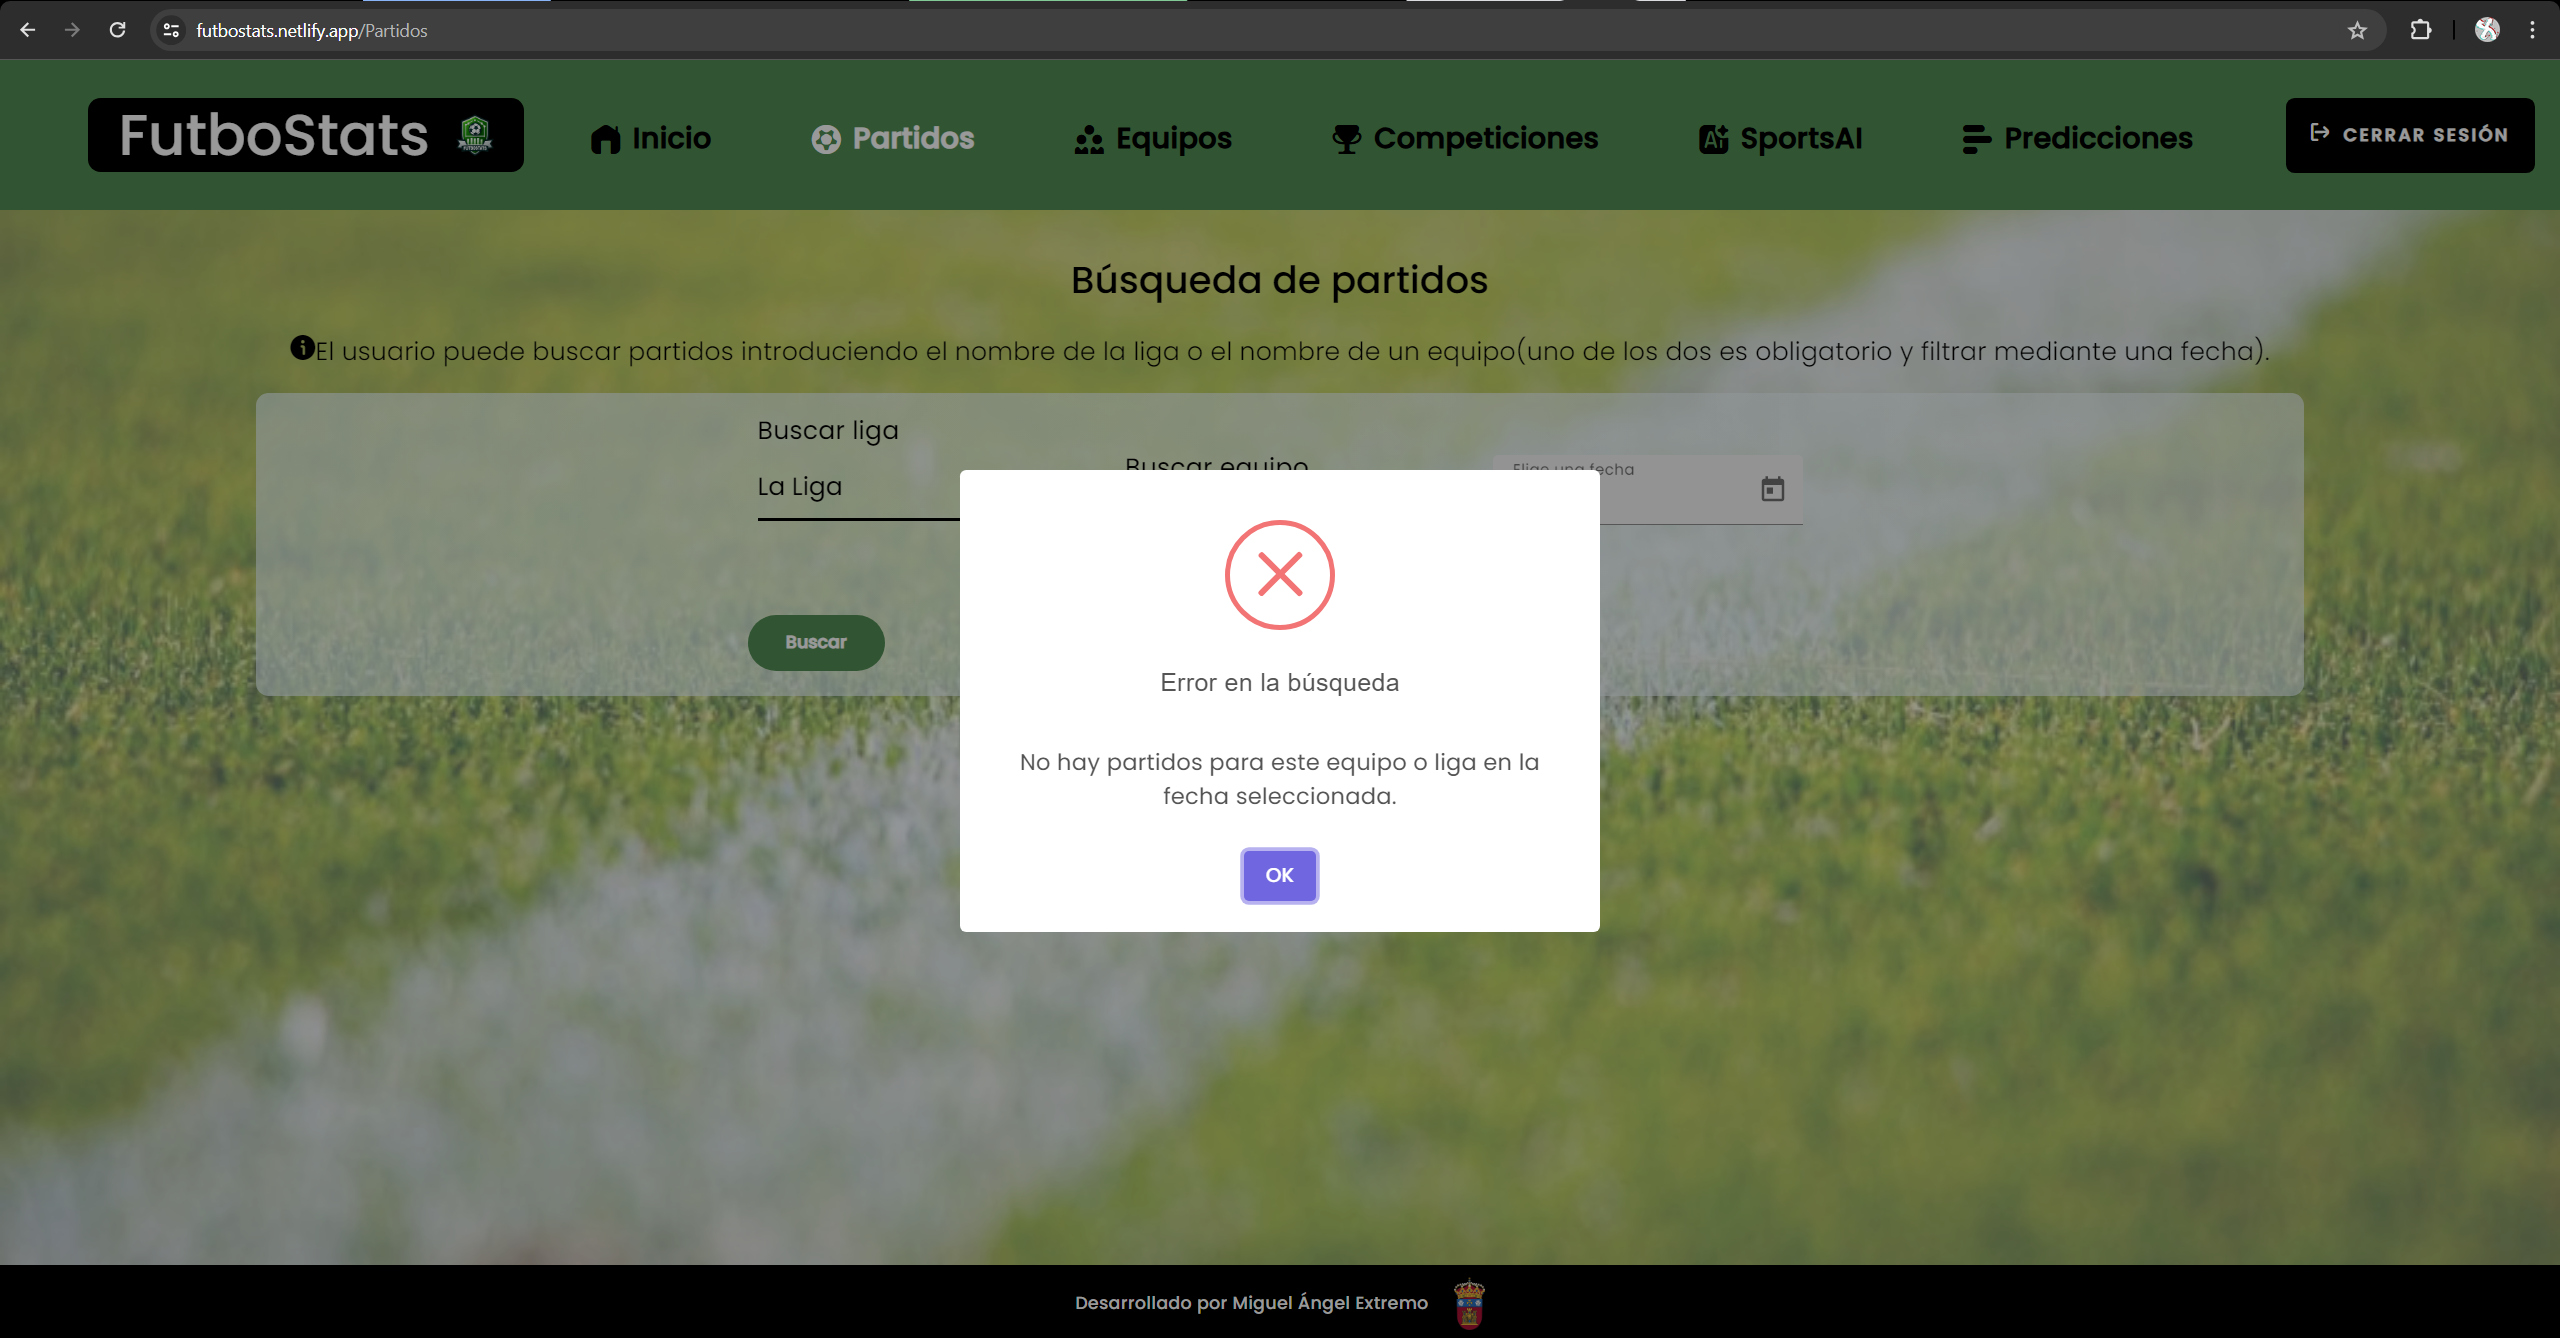
\includegraphics[width=1\linewidth]{img/partidosError-UM.png}
    \caption{Búsqueda de partidos en FutboStats sin resultados.}
    \label{fig:enter-label}
\end{figure}

\subsection{Buscar equipos}
El apartado 'Equipos' de FutboStats proporciona al usuario una forma sencilla de buscar información sobre un equipo de fútbol y consultar algunas estadísticas. \\
Para buscar equipos el usuario debe:
\begin{enumerate}
    \item Pulsar en el menú superior la opción 'Equipos'.
    \item Introducir el nombre de un equipo.
    \item Elegir un año del que quiera ver las estadísticas. Por defecto, se elige el 2023.
    \item Darle a enter o al botón de buscar para realizar la búsqueda.
    \item El usuario visualizará información del equipo como su escudo, año de fundación, estadio, liga, los cuatro partidos anteriores que ha disputado, los cuatro partidos siguientes que ha disputado, la plantilla del equipo, estadísticas sobre las tarjetas rojas y amarillas, goles a favor y en contra, alineaciones más utilizadas, estadísticas de penaltis.
\end{enumerate}

\begin{figure}[H]
    \centering
    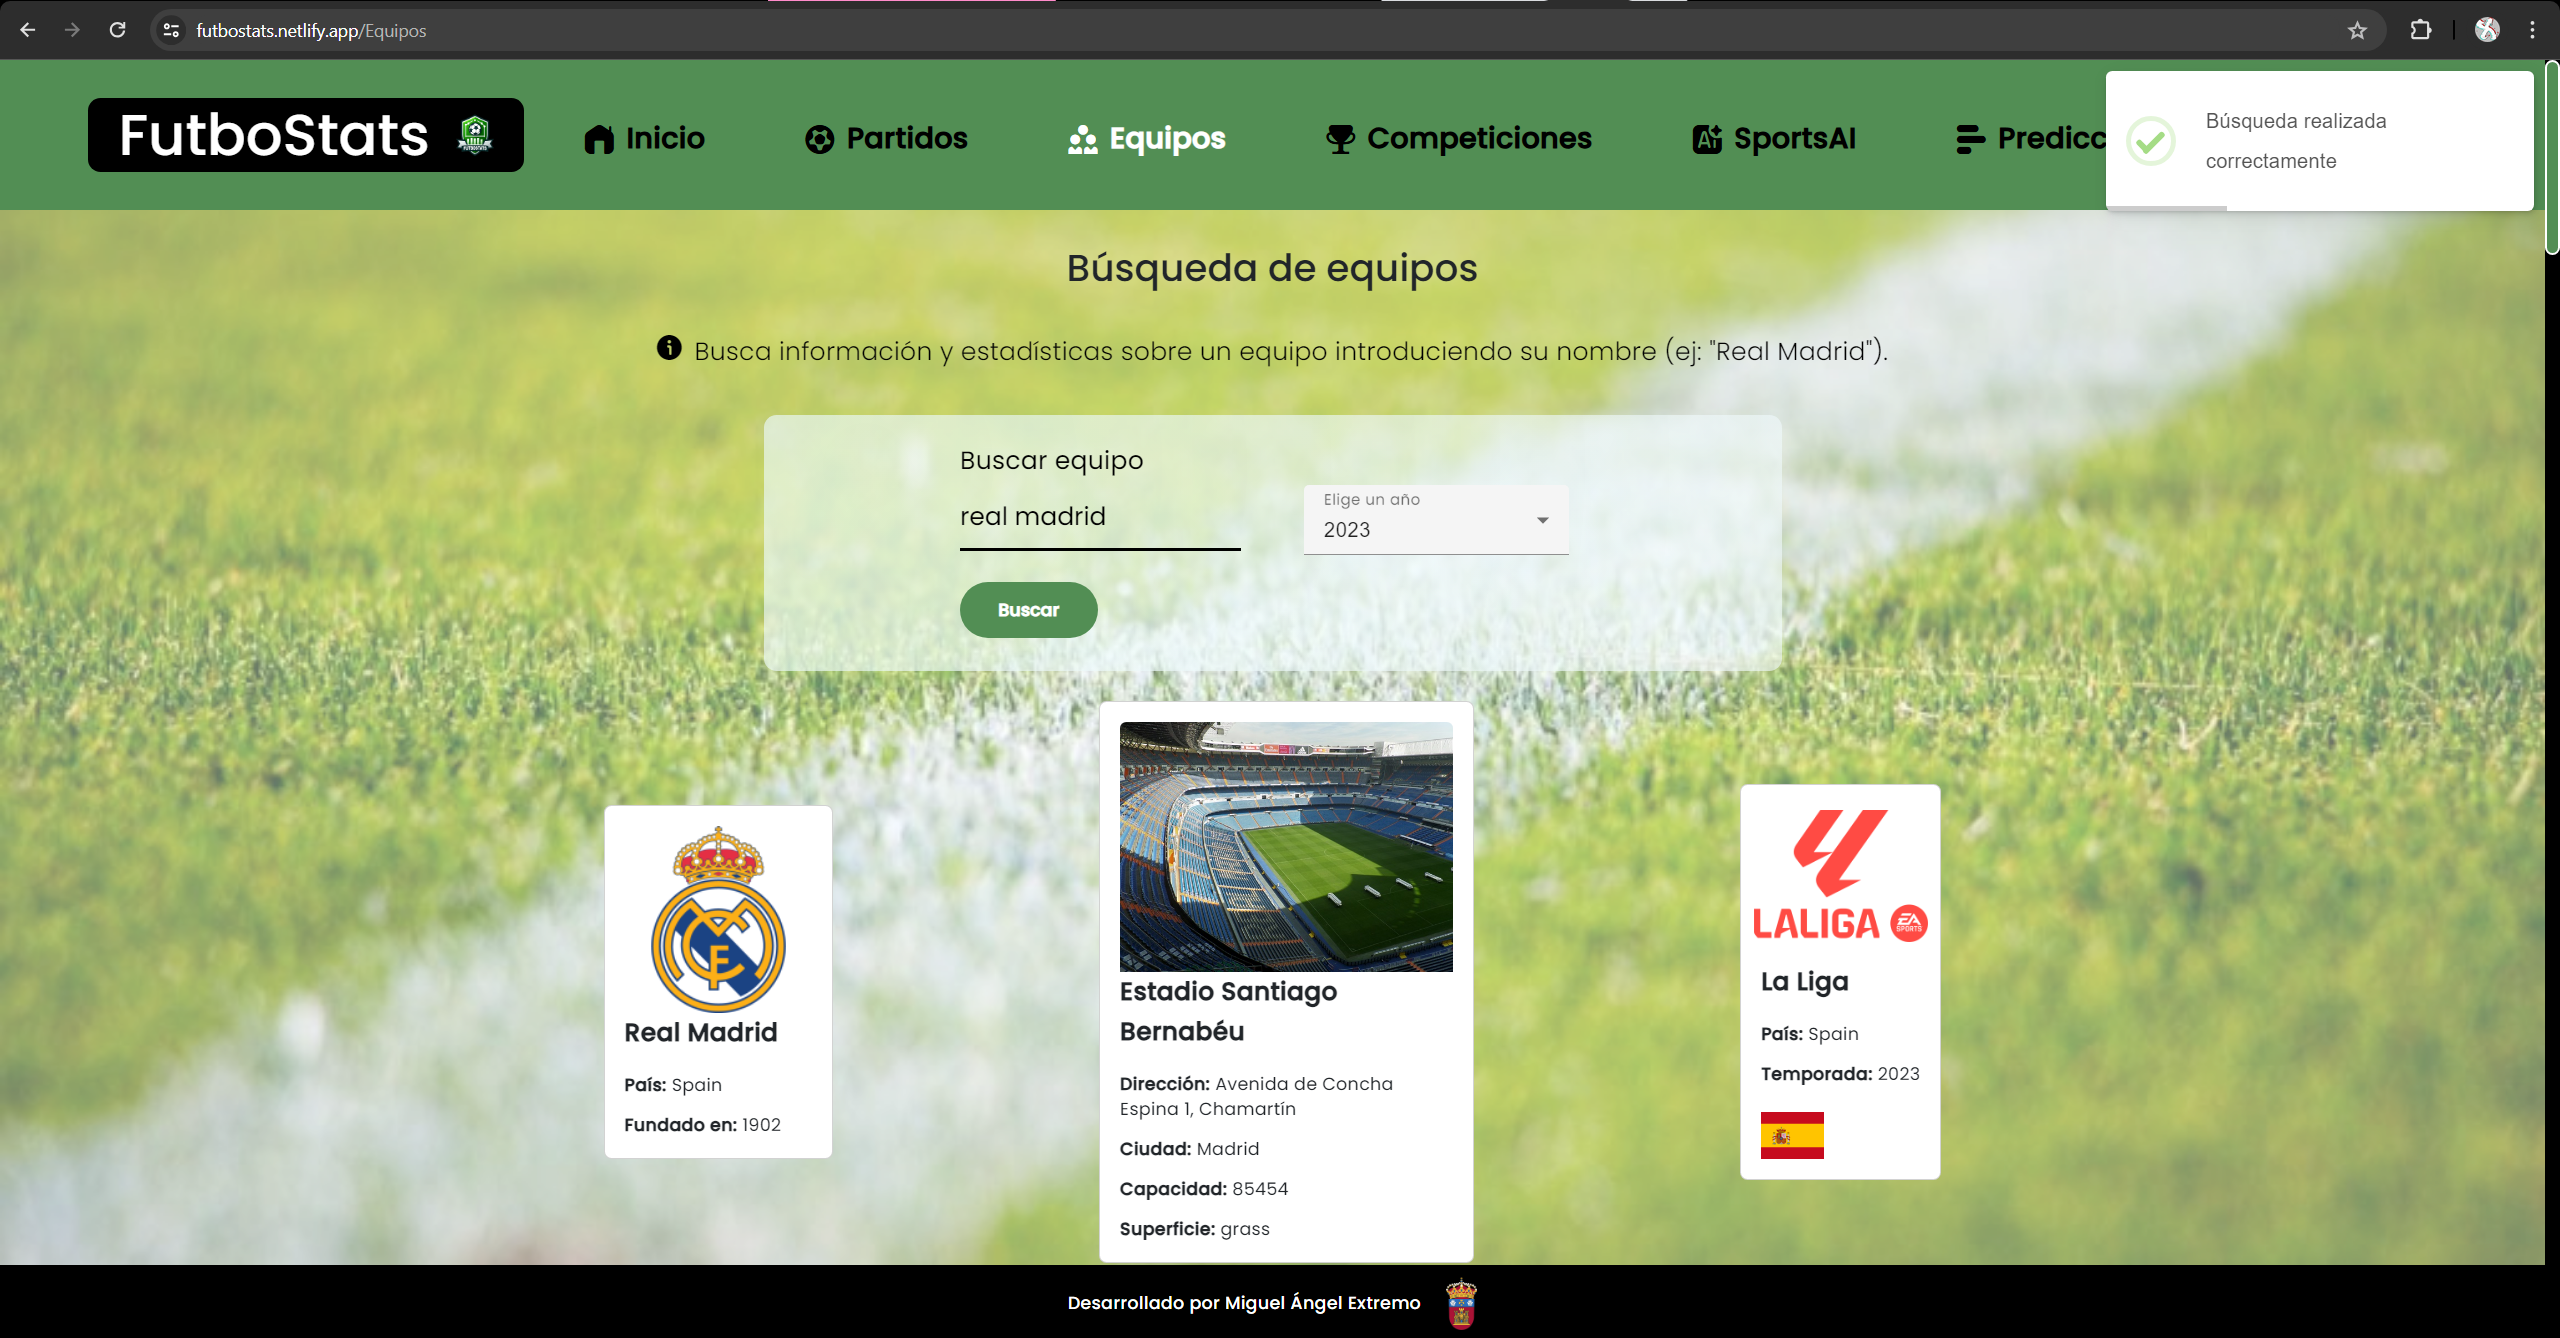
\includegraphics[width=1\linewidth]{img/busquedaEquipos.png}
    \caption{Búsqueda de equipos en FutboStats.}
    \label{fig:enter-label}
\end{figure}



\subsection{Buscar clasificaciones}
El apartado 'Competiciones' de FutboStats permite al usuario consultar la clasificación de una liga de forma sencilla. \\
Para buscar clasificaciones el usuario debe:
\begin{enumerate}
    \item Pulsar en el menú superior la opción 'Competiciones'.
    \item Introducir el nombre de la competición. El sistema genera una lista de sugerencias al usuario a medida que este escribe.
    \item Pulsar en una de las sugerencias y dar al botón de buscar.
    \item Elegir el año del que se quiere ver la clasificación. Por defecto se elige el 2023.
    \item El usuario visualizará una tabla que muestra la clasificación de la liga seleccionada.
    \item Si se cambia el año, la tabla cambiará para mostrar la información del nuevo año seleccionado.
\end{enumerate}

\begin{figure}[H]
    \centering
    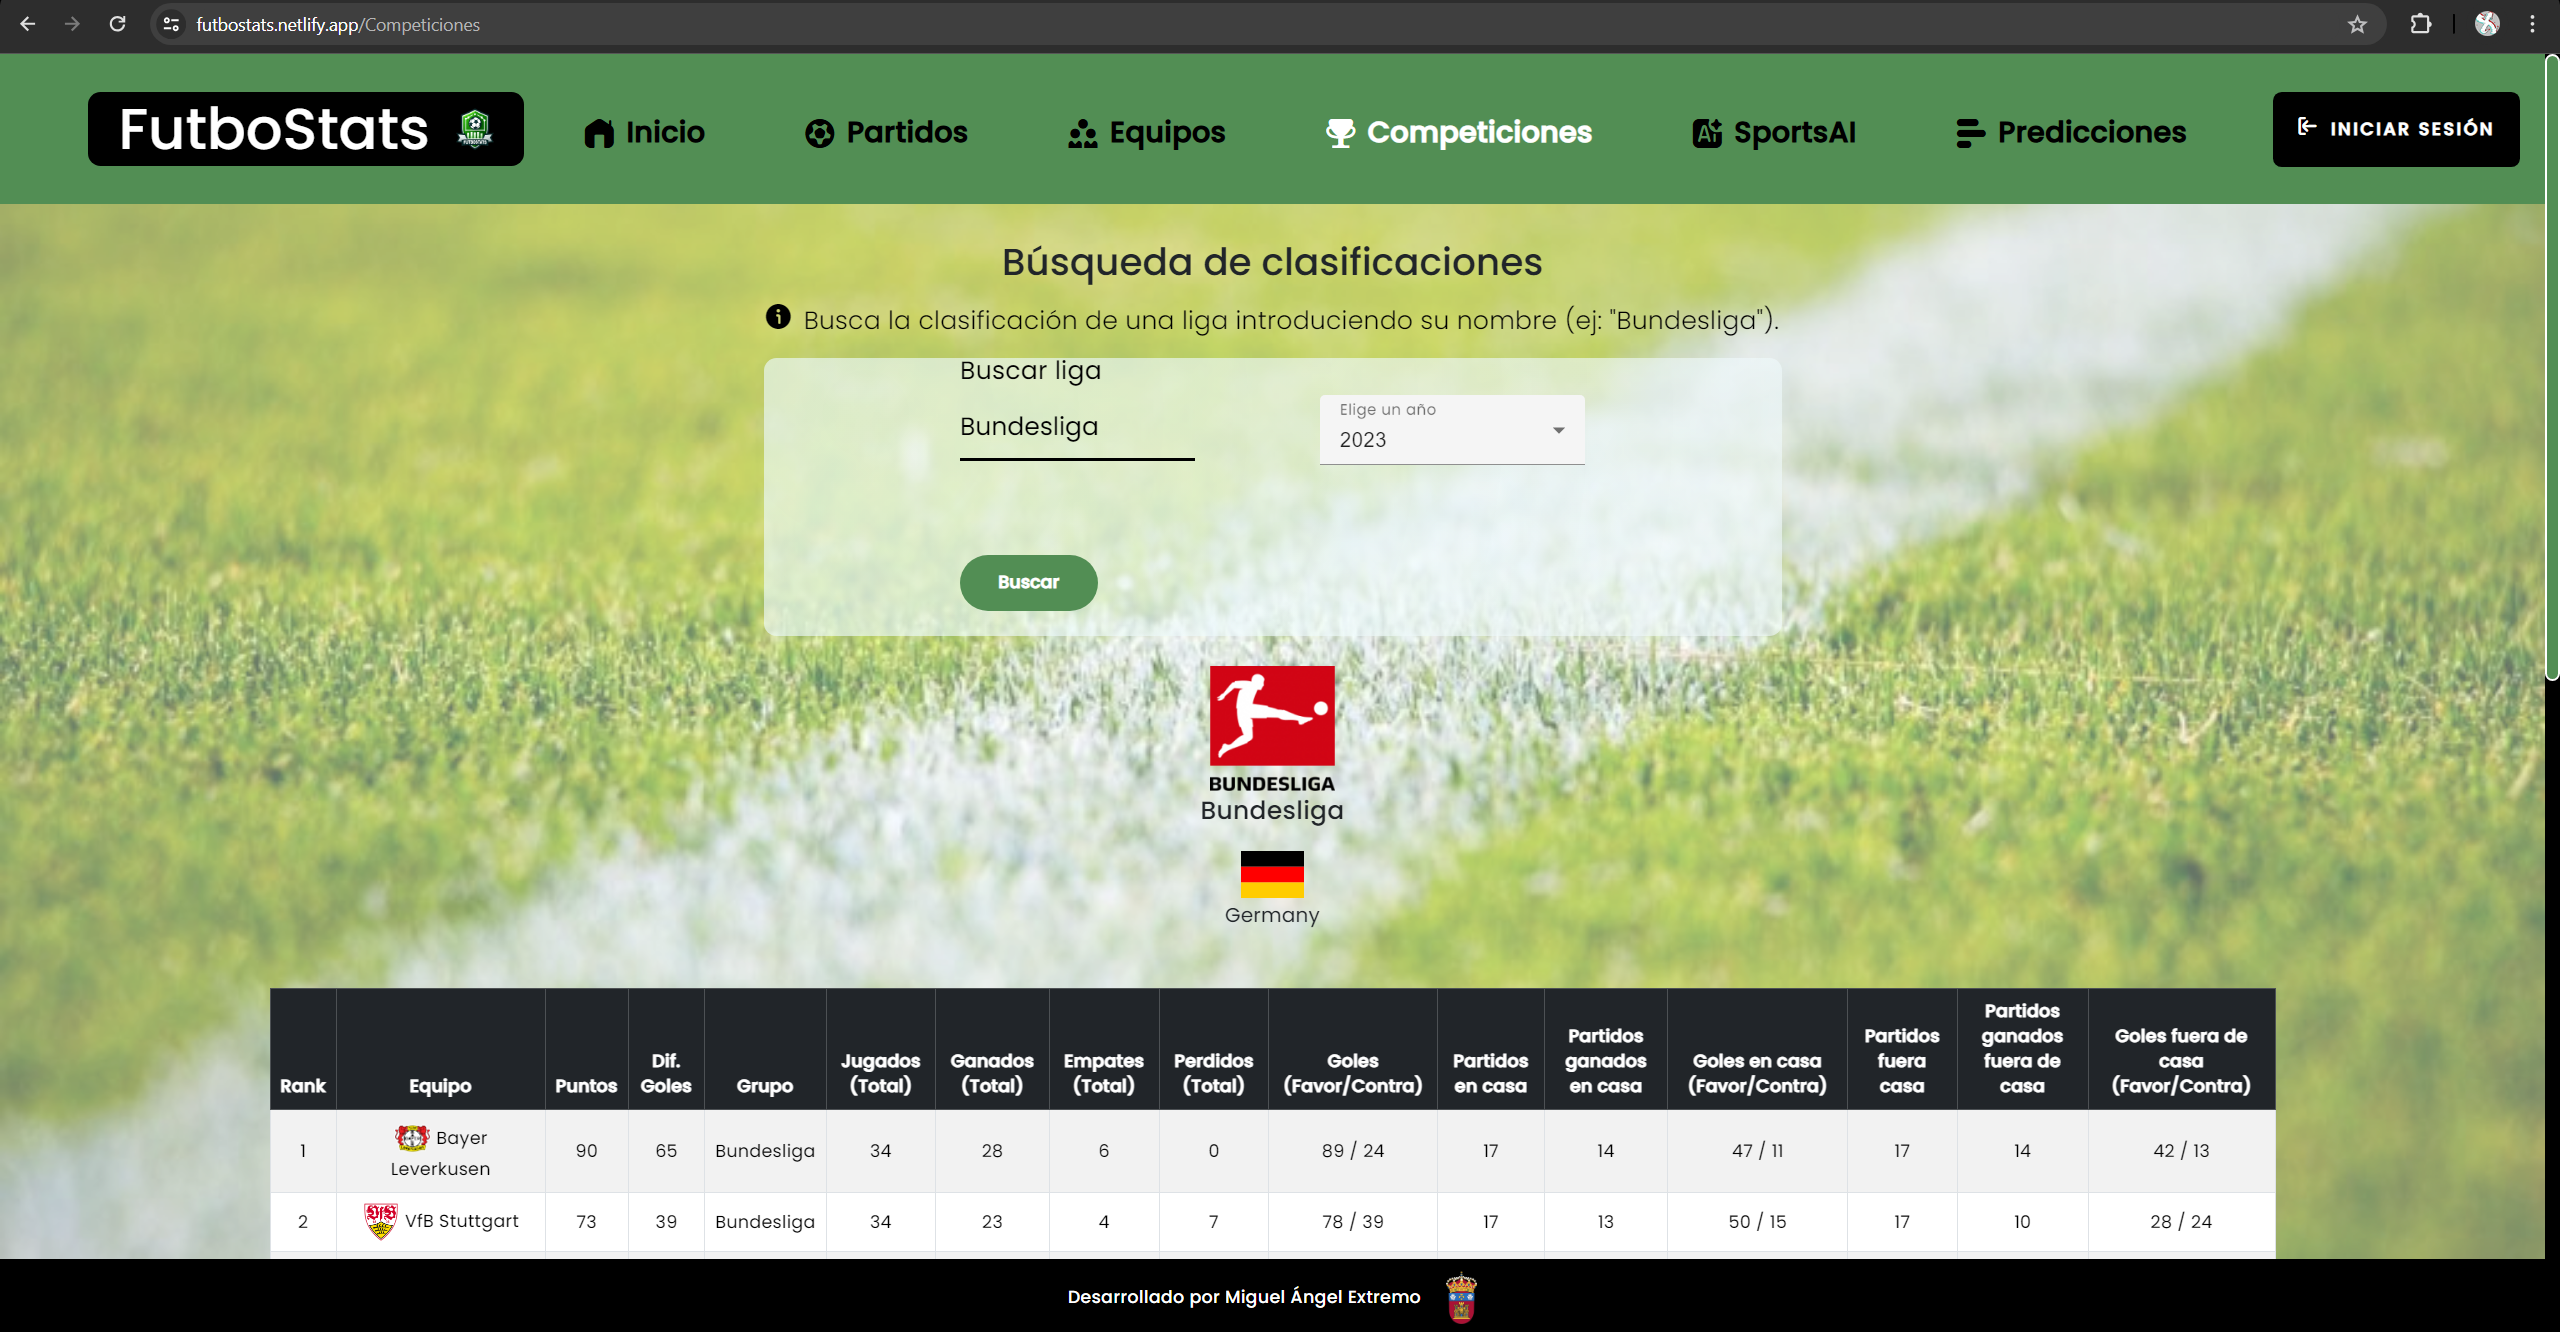
\includegraphics[width=1\linewidth]{img/buscarCompeticiones.png}
    \caption{Búsqueda de competiciones en FutboStats.}
    \label{fig:enter-label}
\end{figure}

\subsection{Iniciar sesión en FutboStats}
Si el usuario quiere utilizar las opciones 'SportsAI' y 'Predicciones' deberá iniciar sesión en la aplicación. La forma de iniciar sesión es muy sencilla, para ello el usuario deberá:
\begin{enumerate}
    \item Pulsar en el botón de iniciar sesión o en las opciones 'SportsAI' o 'Predicciones', las cuáles al no estar autenticado redirigen al usuario a la pantalla de inicio de sesión.
    \item En la pantalla de iniciar sesión, pulsar de nuevo en el botón 'Iniciar sesión' dentro del recuadro debajo del logotipo de Google.
    \item Se redirige al usuario para que se registre con su cuenta de Google.
    \item Una vez registrado, se redirige al usuario de nuevo a la página de 'Inicio' de FutboStats.
    \item El usuario puede acceder a las funcionalidades protegidas de la aplicación.
\end{enumerate}

\begin{figure}[H]
    \centering
    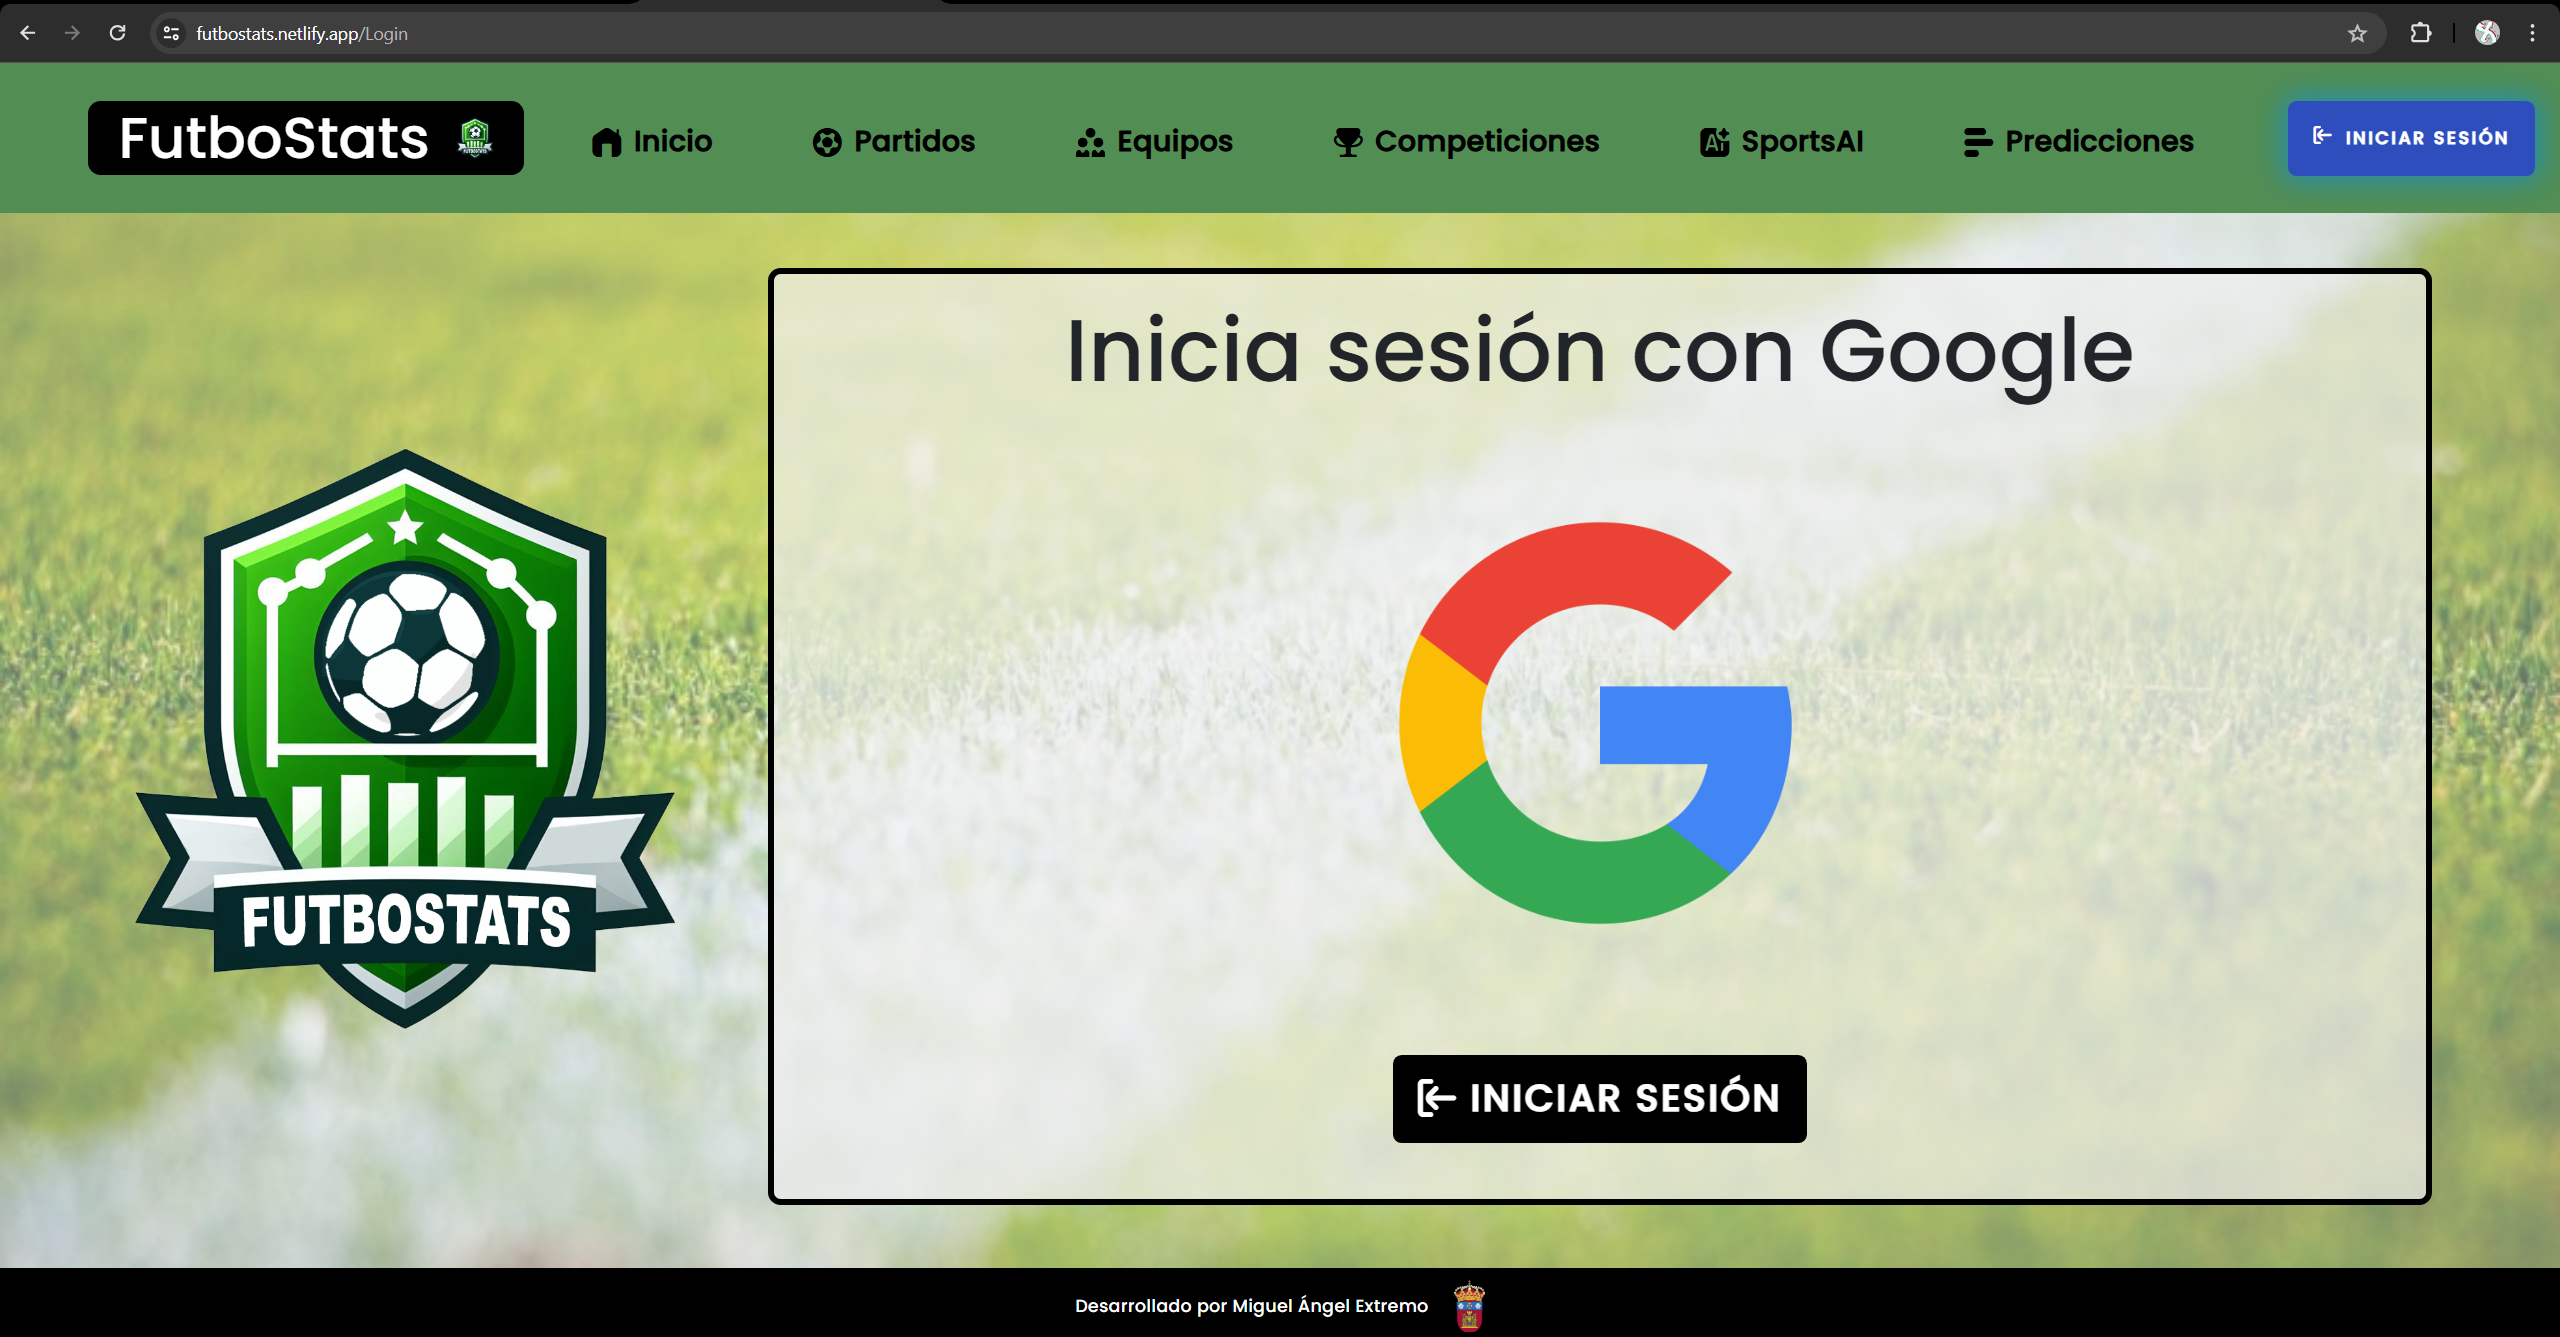
\includegraphics[width=1\linewidth]{img/iniciarSesion-UM.png}
    \caption{Paso 1 de iniciar sesión en FutboStats: entrar en iniciar sesión.}
    \label{fig:enter-label}
\end{figure}

\begin{figure}[H]
    \centering
    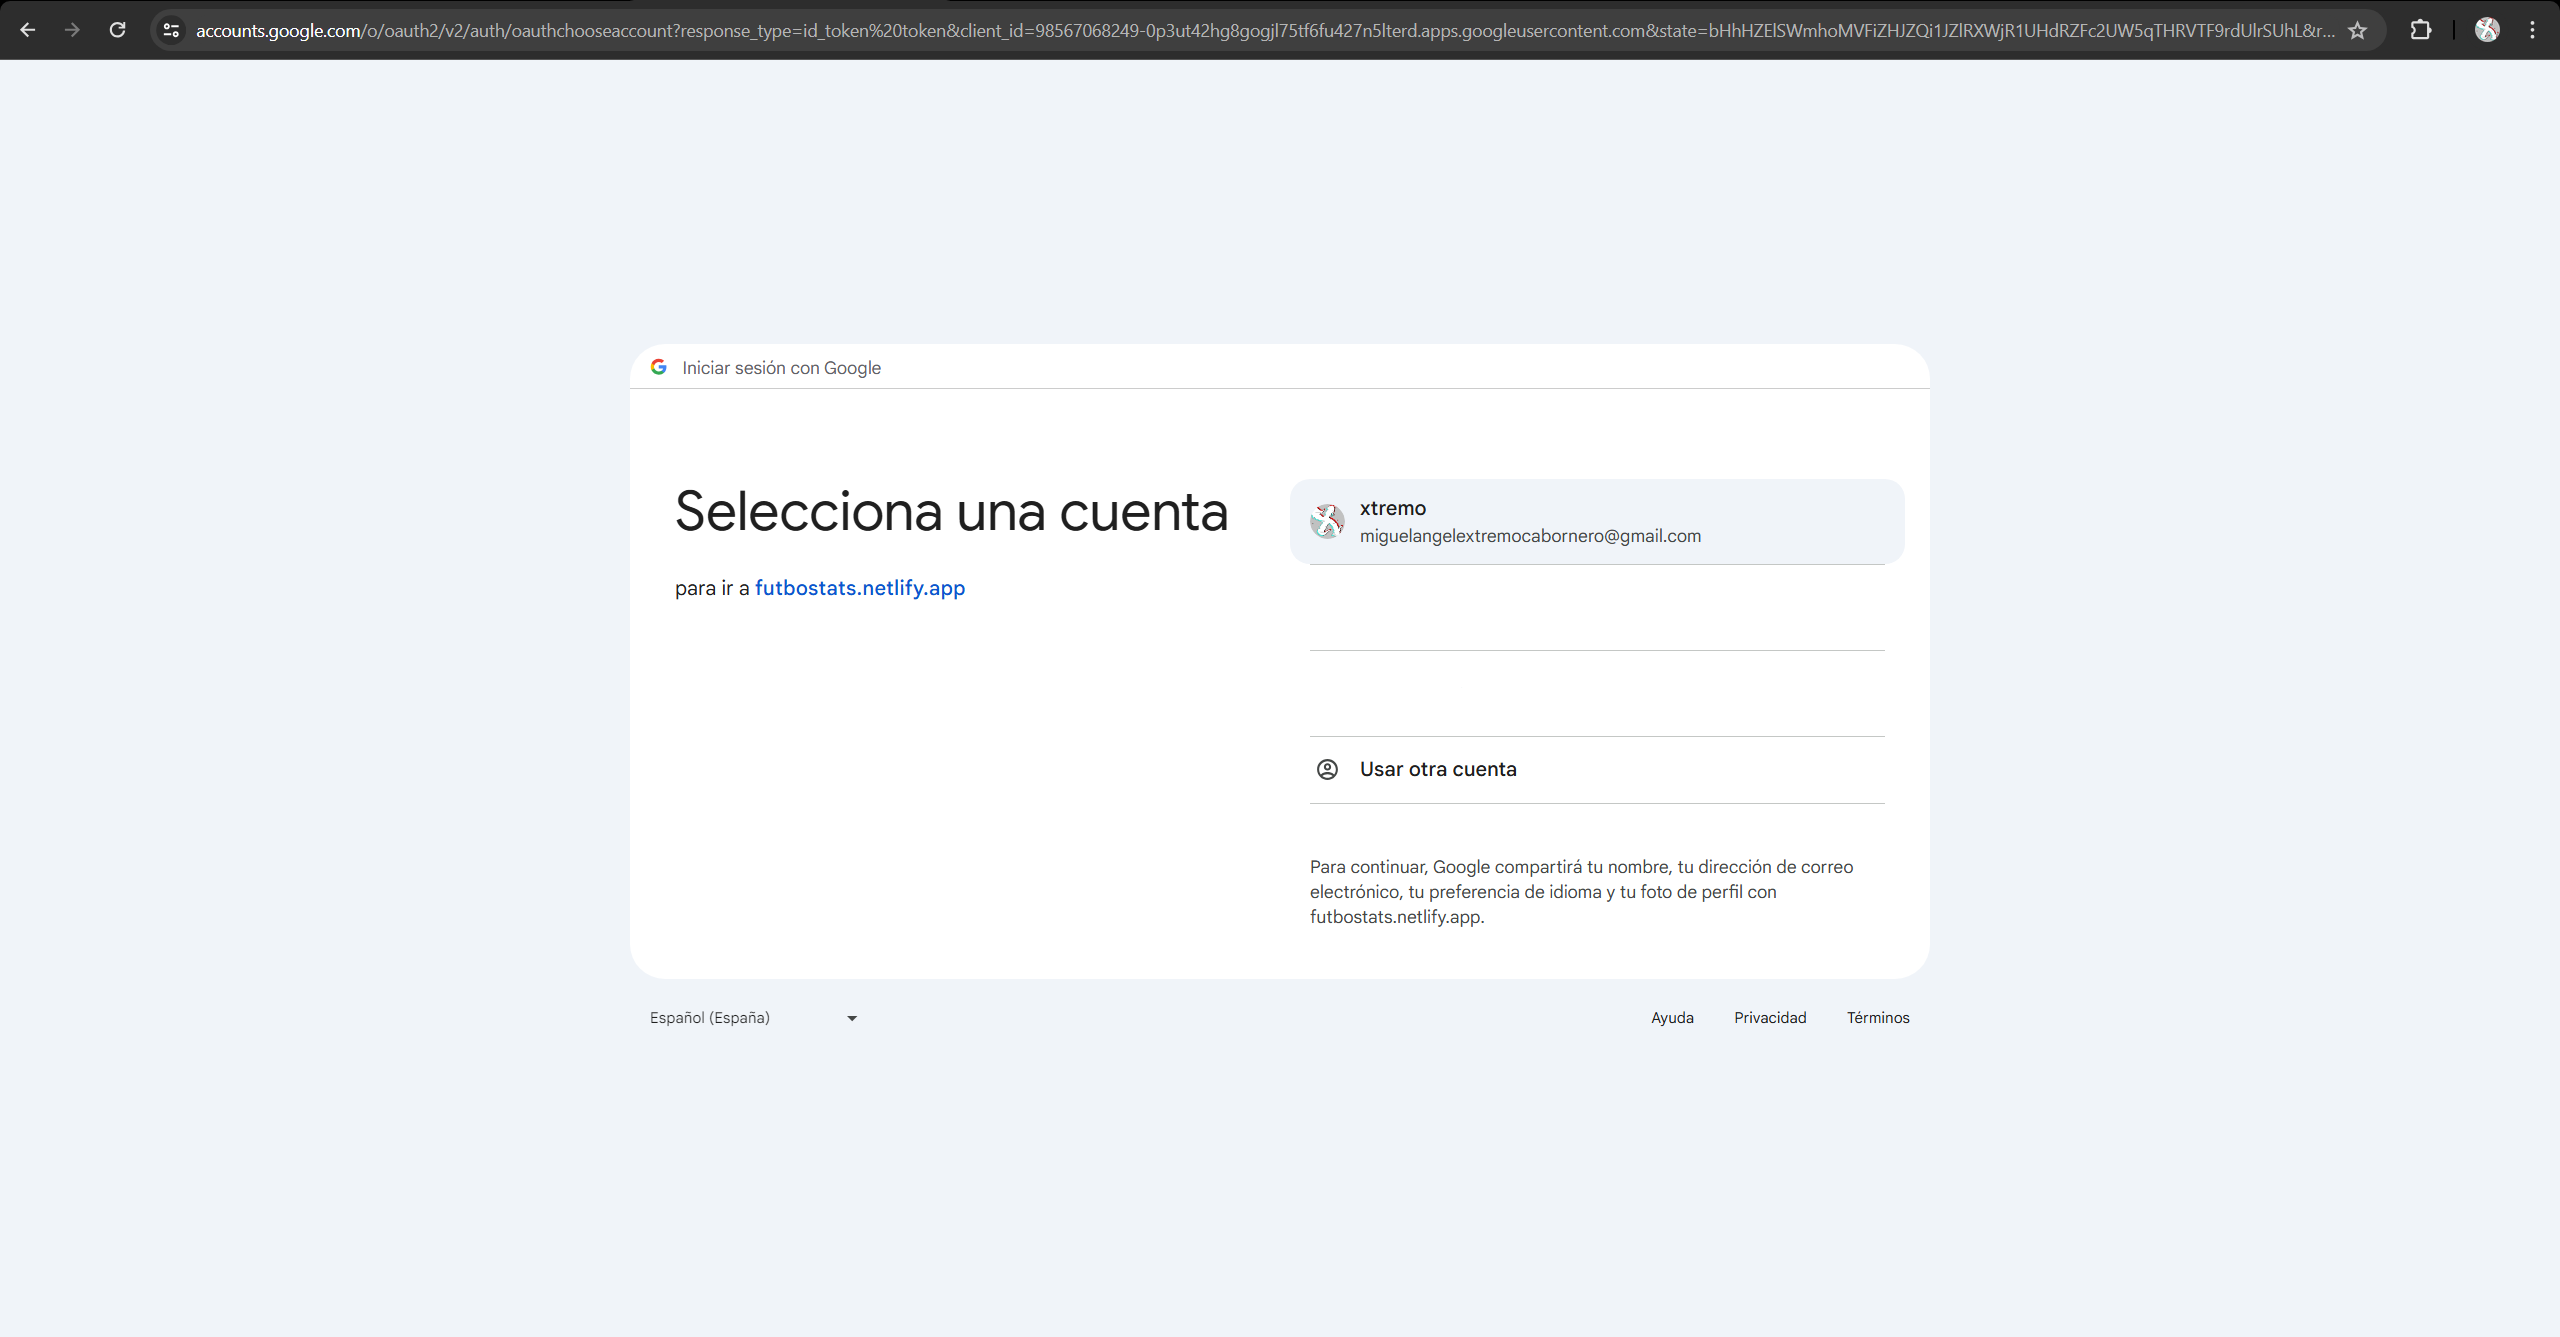
\includegraphics[width=1\linewidth]{img/iniciarSesion2-UM.png}
    \caption{Paso 2 de iniciar sesión en FutboStats: elegir la cuenta de Google.}
    \label{fig:enter-label}
\end{figure}

\begin{figure}[H]
    \centering
    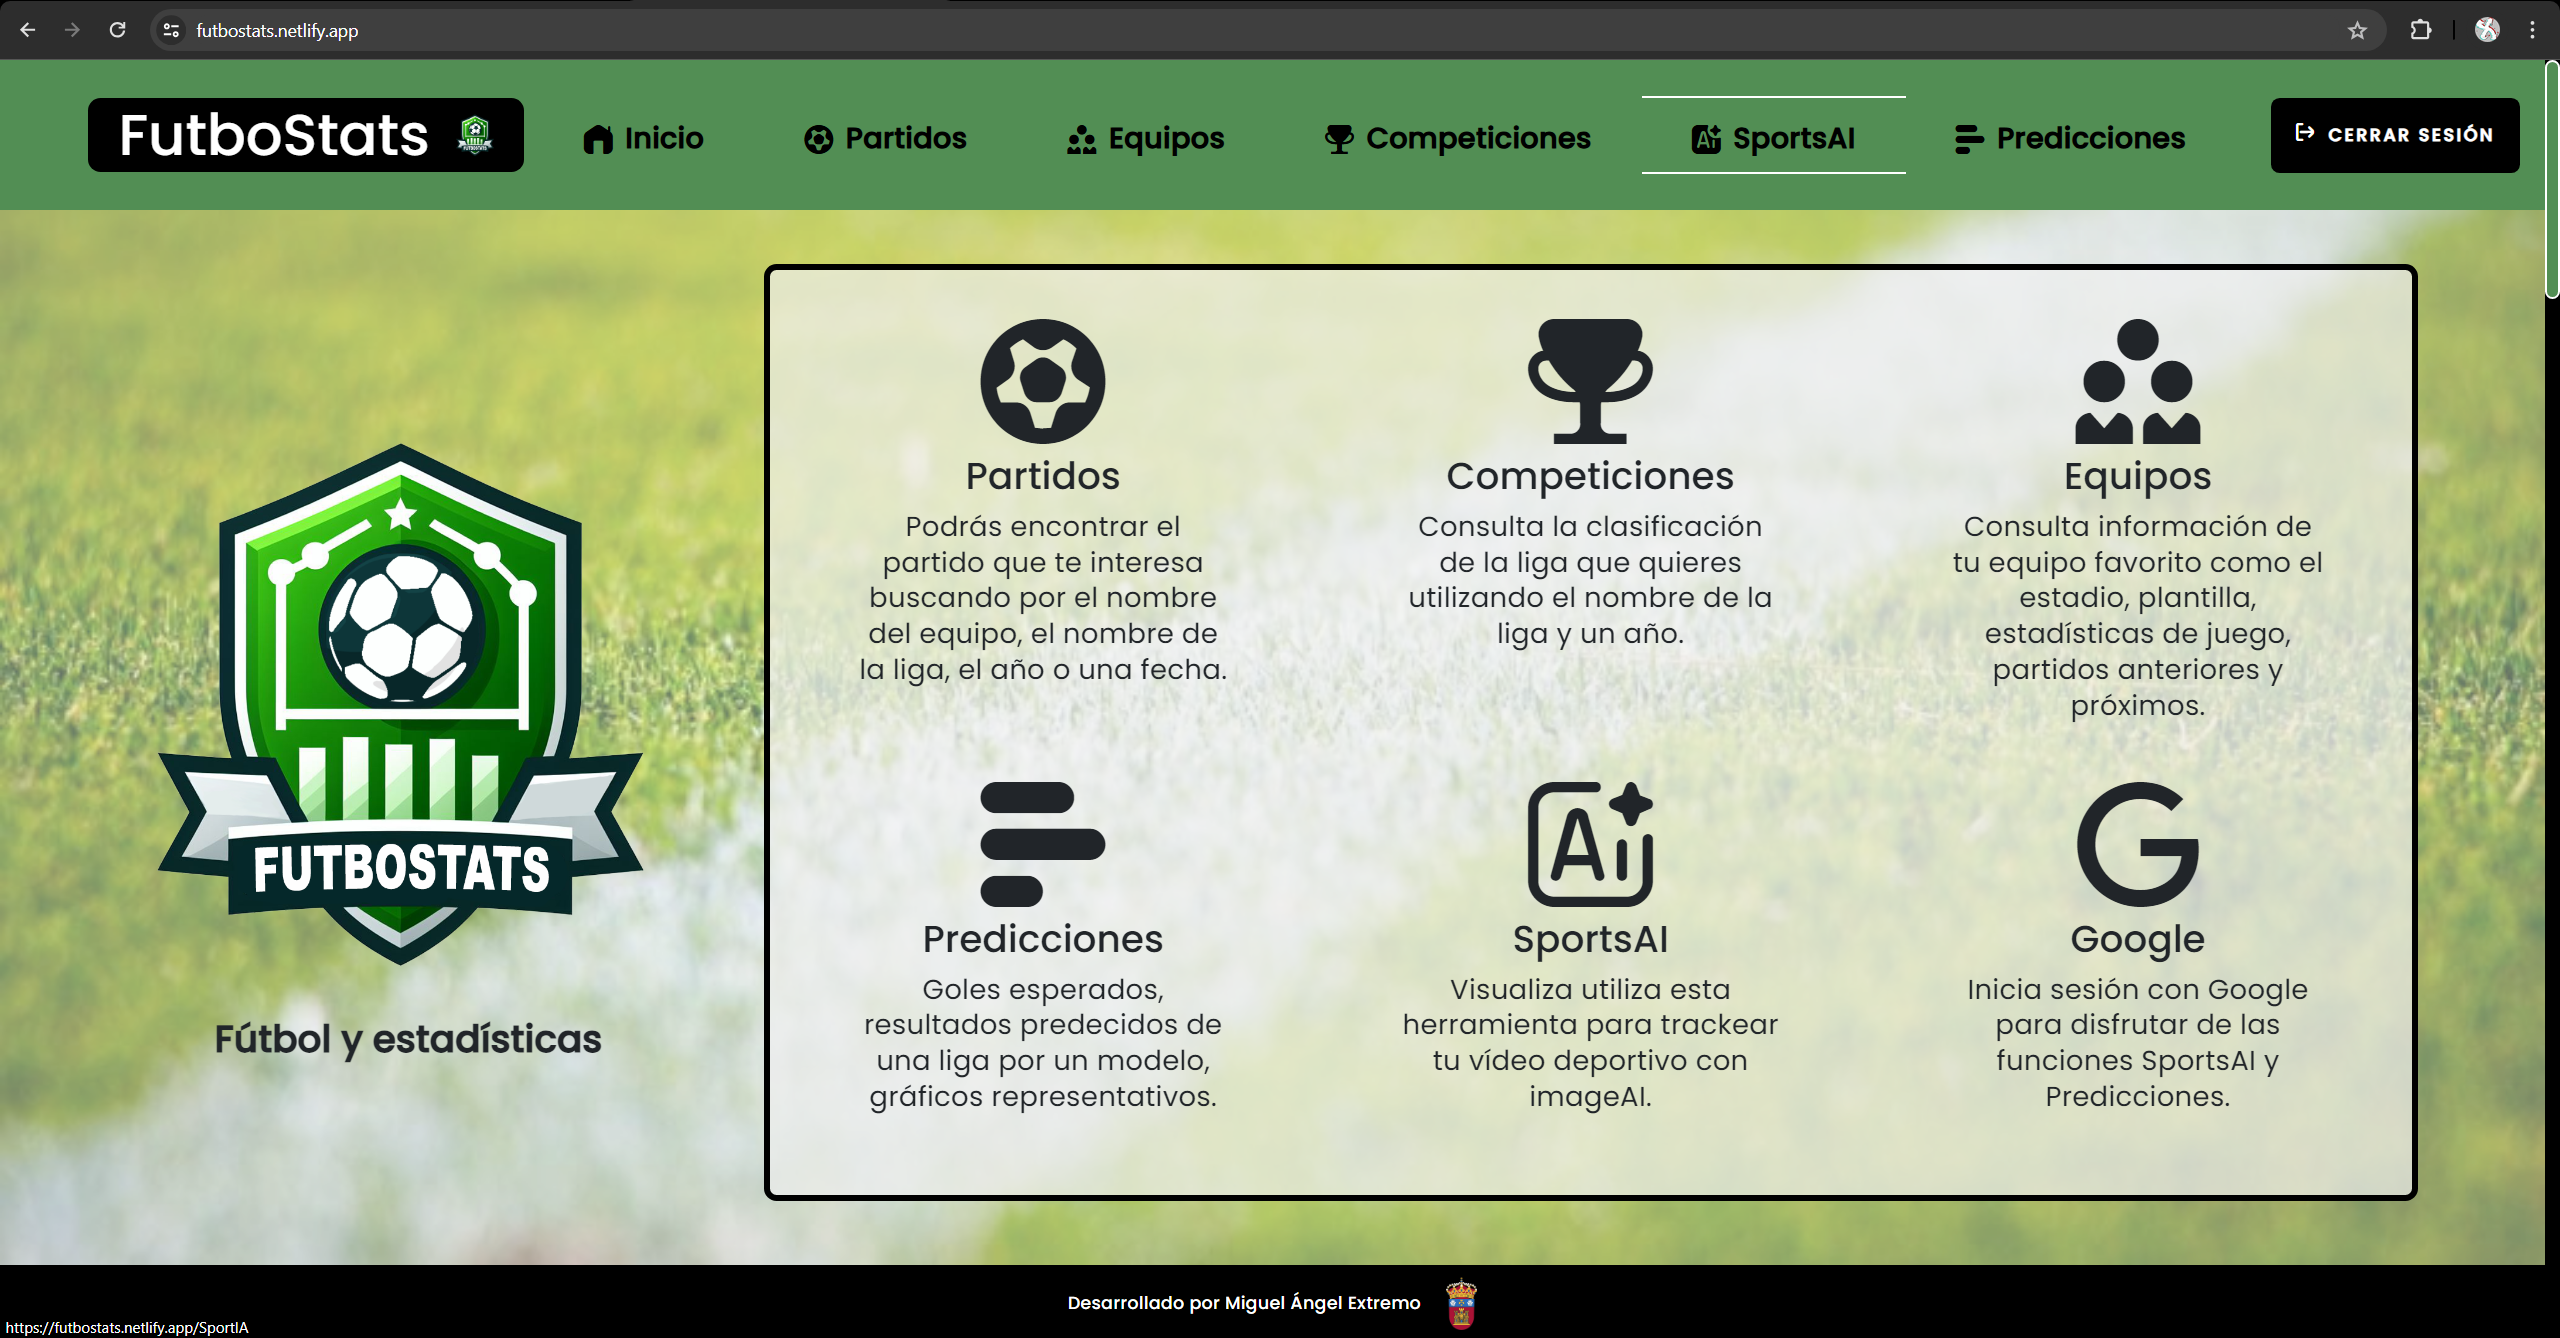
\includegraphics[width=1\linewidth]{img/iniciarSesion3-UM.png}
    \caption{Paso 3 de iniciar sesión en FutboStats: autenticado con éxito.}
    \label{fig:enter-label}
\end{figure}

\subsection{Cerrar sesión en FutboStats}
Si el usuario desea cerrar la sesión en FutboStats seguirá los siguientes pasos.
\begin{enumerate}
    \item Pulsar en el botón de 'Cerrar sesión'.
    \item Se mostrará una modal con dos opciones: cerrar sesión o cancelar.
    \item Si el usuario acepta cerrar sesión se cierra la sesión y no puede acceder a las funcionalidades protegidas de la aplicación.
    \item Si el usuario cancela cerrar sesión puede seguir accediendo a las funcionalidades protegidas de la aplicación.
\end{enumerate}
\begin{figure}[H]
    \centering
    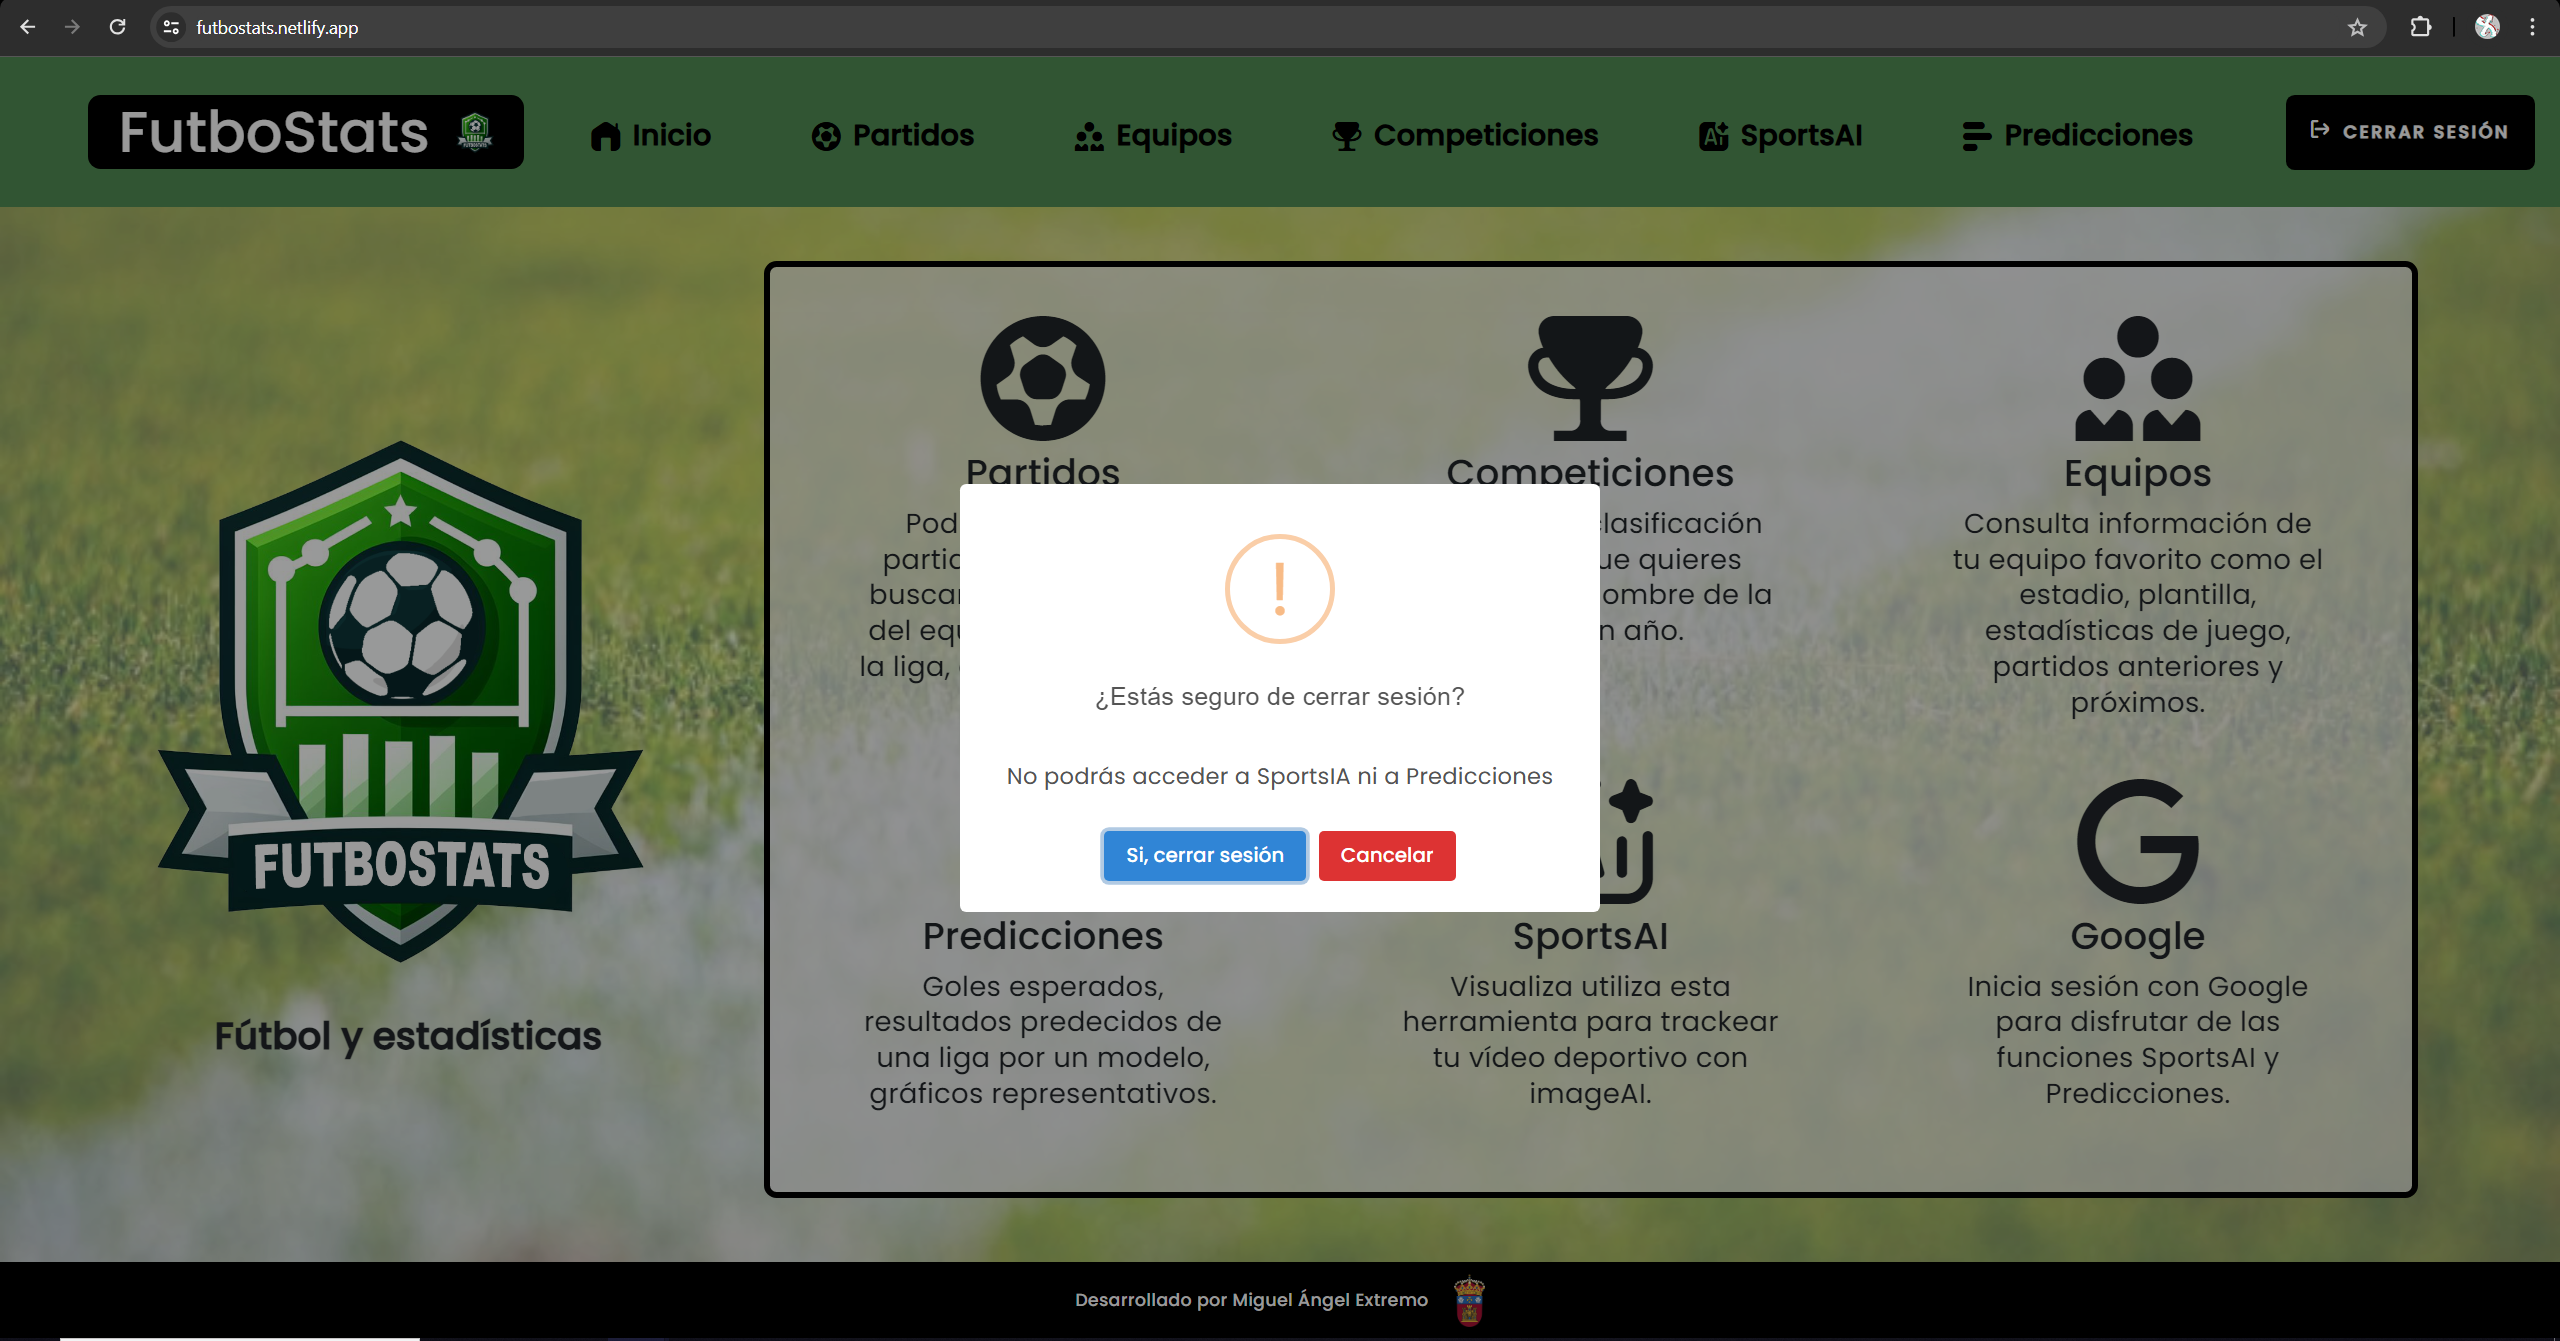
\includegraphics[width=1\linewidth]{img/cerrarSesion-UM.png}
    \caption{Cerrar sesión en FutboStats.}
    \label{fig:enter-label}
\end{figure}

\subsection{Utilizar SportAI en FutboStats}
En la opción 'SportsAI' de FutboStats el usuario podrá subir un vídeo suyo en la aplicación y obtener un vídeo con el procesado de imageAI. \\
Los pasos que debe seguir para utilizar esta funcionalidad son:
\begin{enumerate}
    \item Iniciar sesión en la aplicación.
    \item Pulsar en la opción 'SportsAI' del menú superior.
    \item Hacer click para elegir o arrastrar un vídeo en formato '.mp4'.
    \item Esperar a que la aplicación genere el vídeo procesado por imageAI.
    \item El usuario podrá visualizar el vídeo nuevo en la aplicación.
\end{enumerate}

\begin{figure}[H]
    \centering
    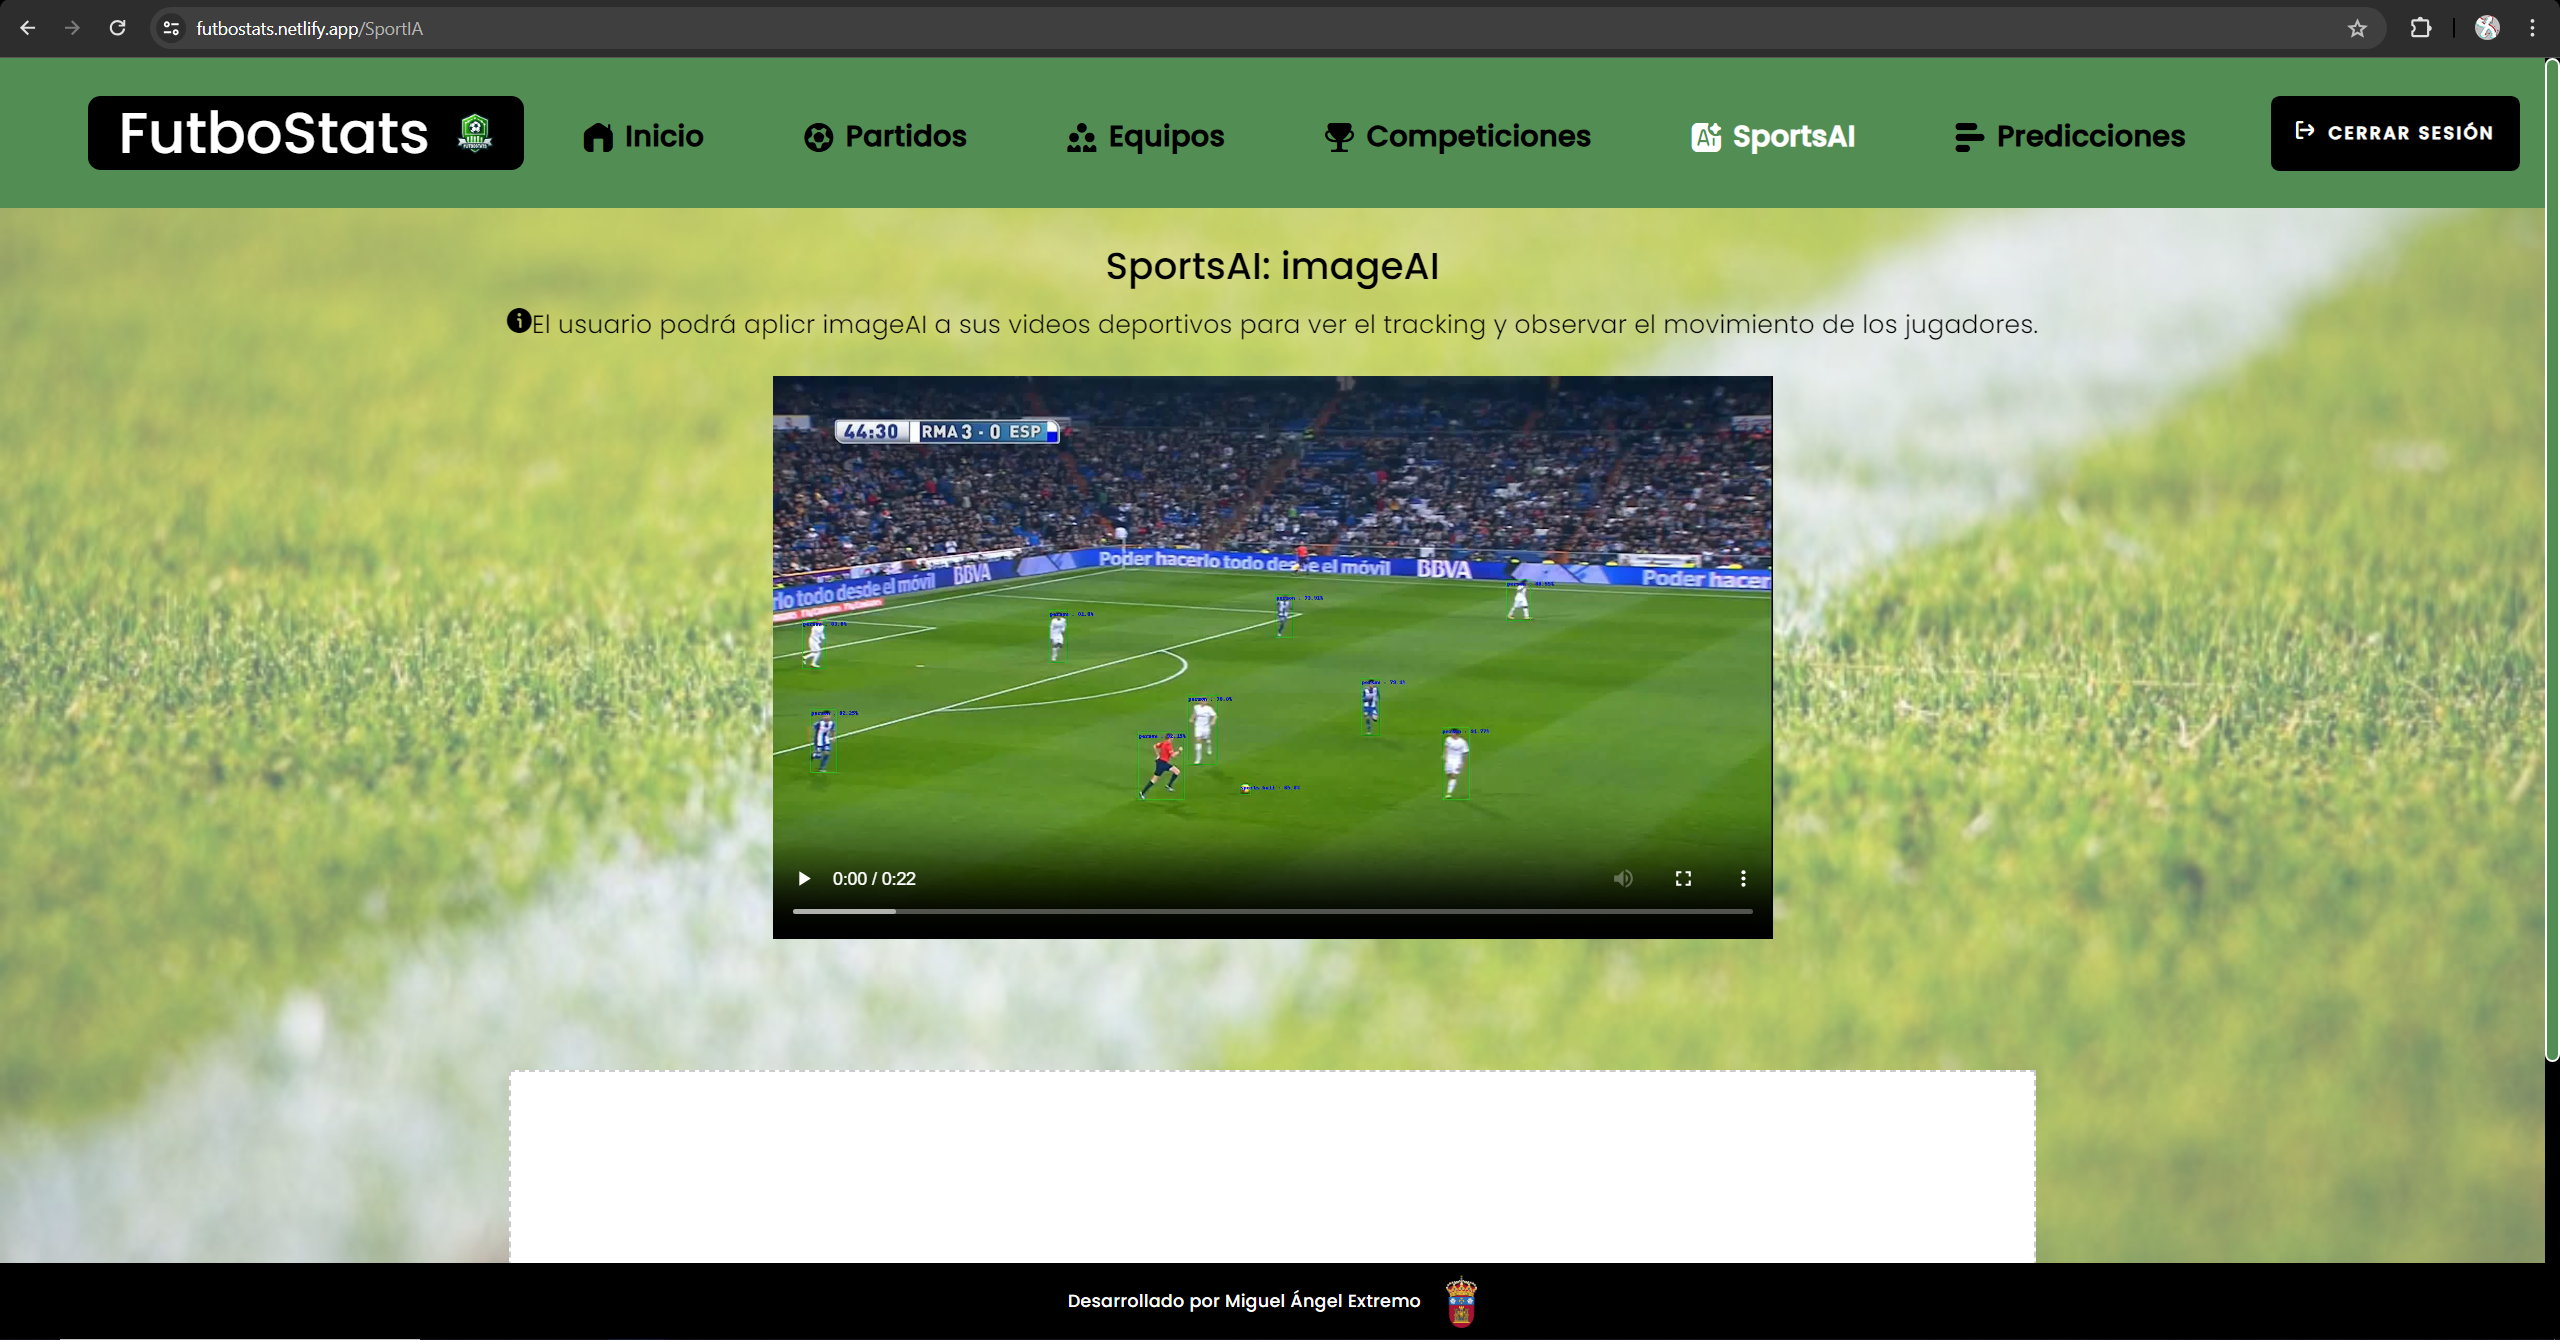
\includegraphics[width=1\linewidth]{img/sportsAI-UM.png}
    \caption{Paso 1 para utilizar SportAI: entrar en 'SportsAI'.}
    \label{fig:enter-label}
\end{figure}

\begin{figure}[H]
    \centering
    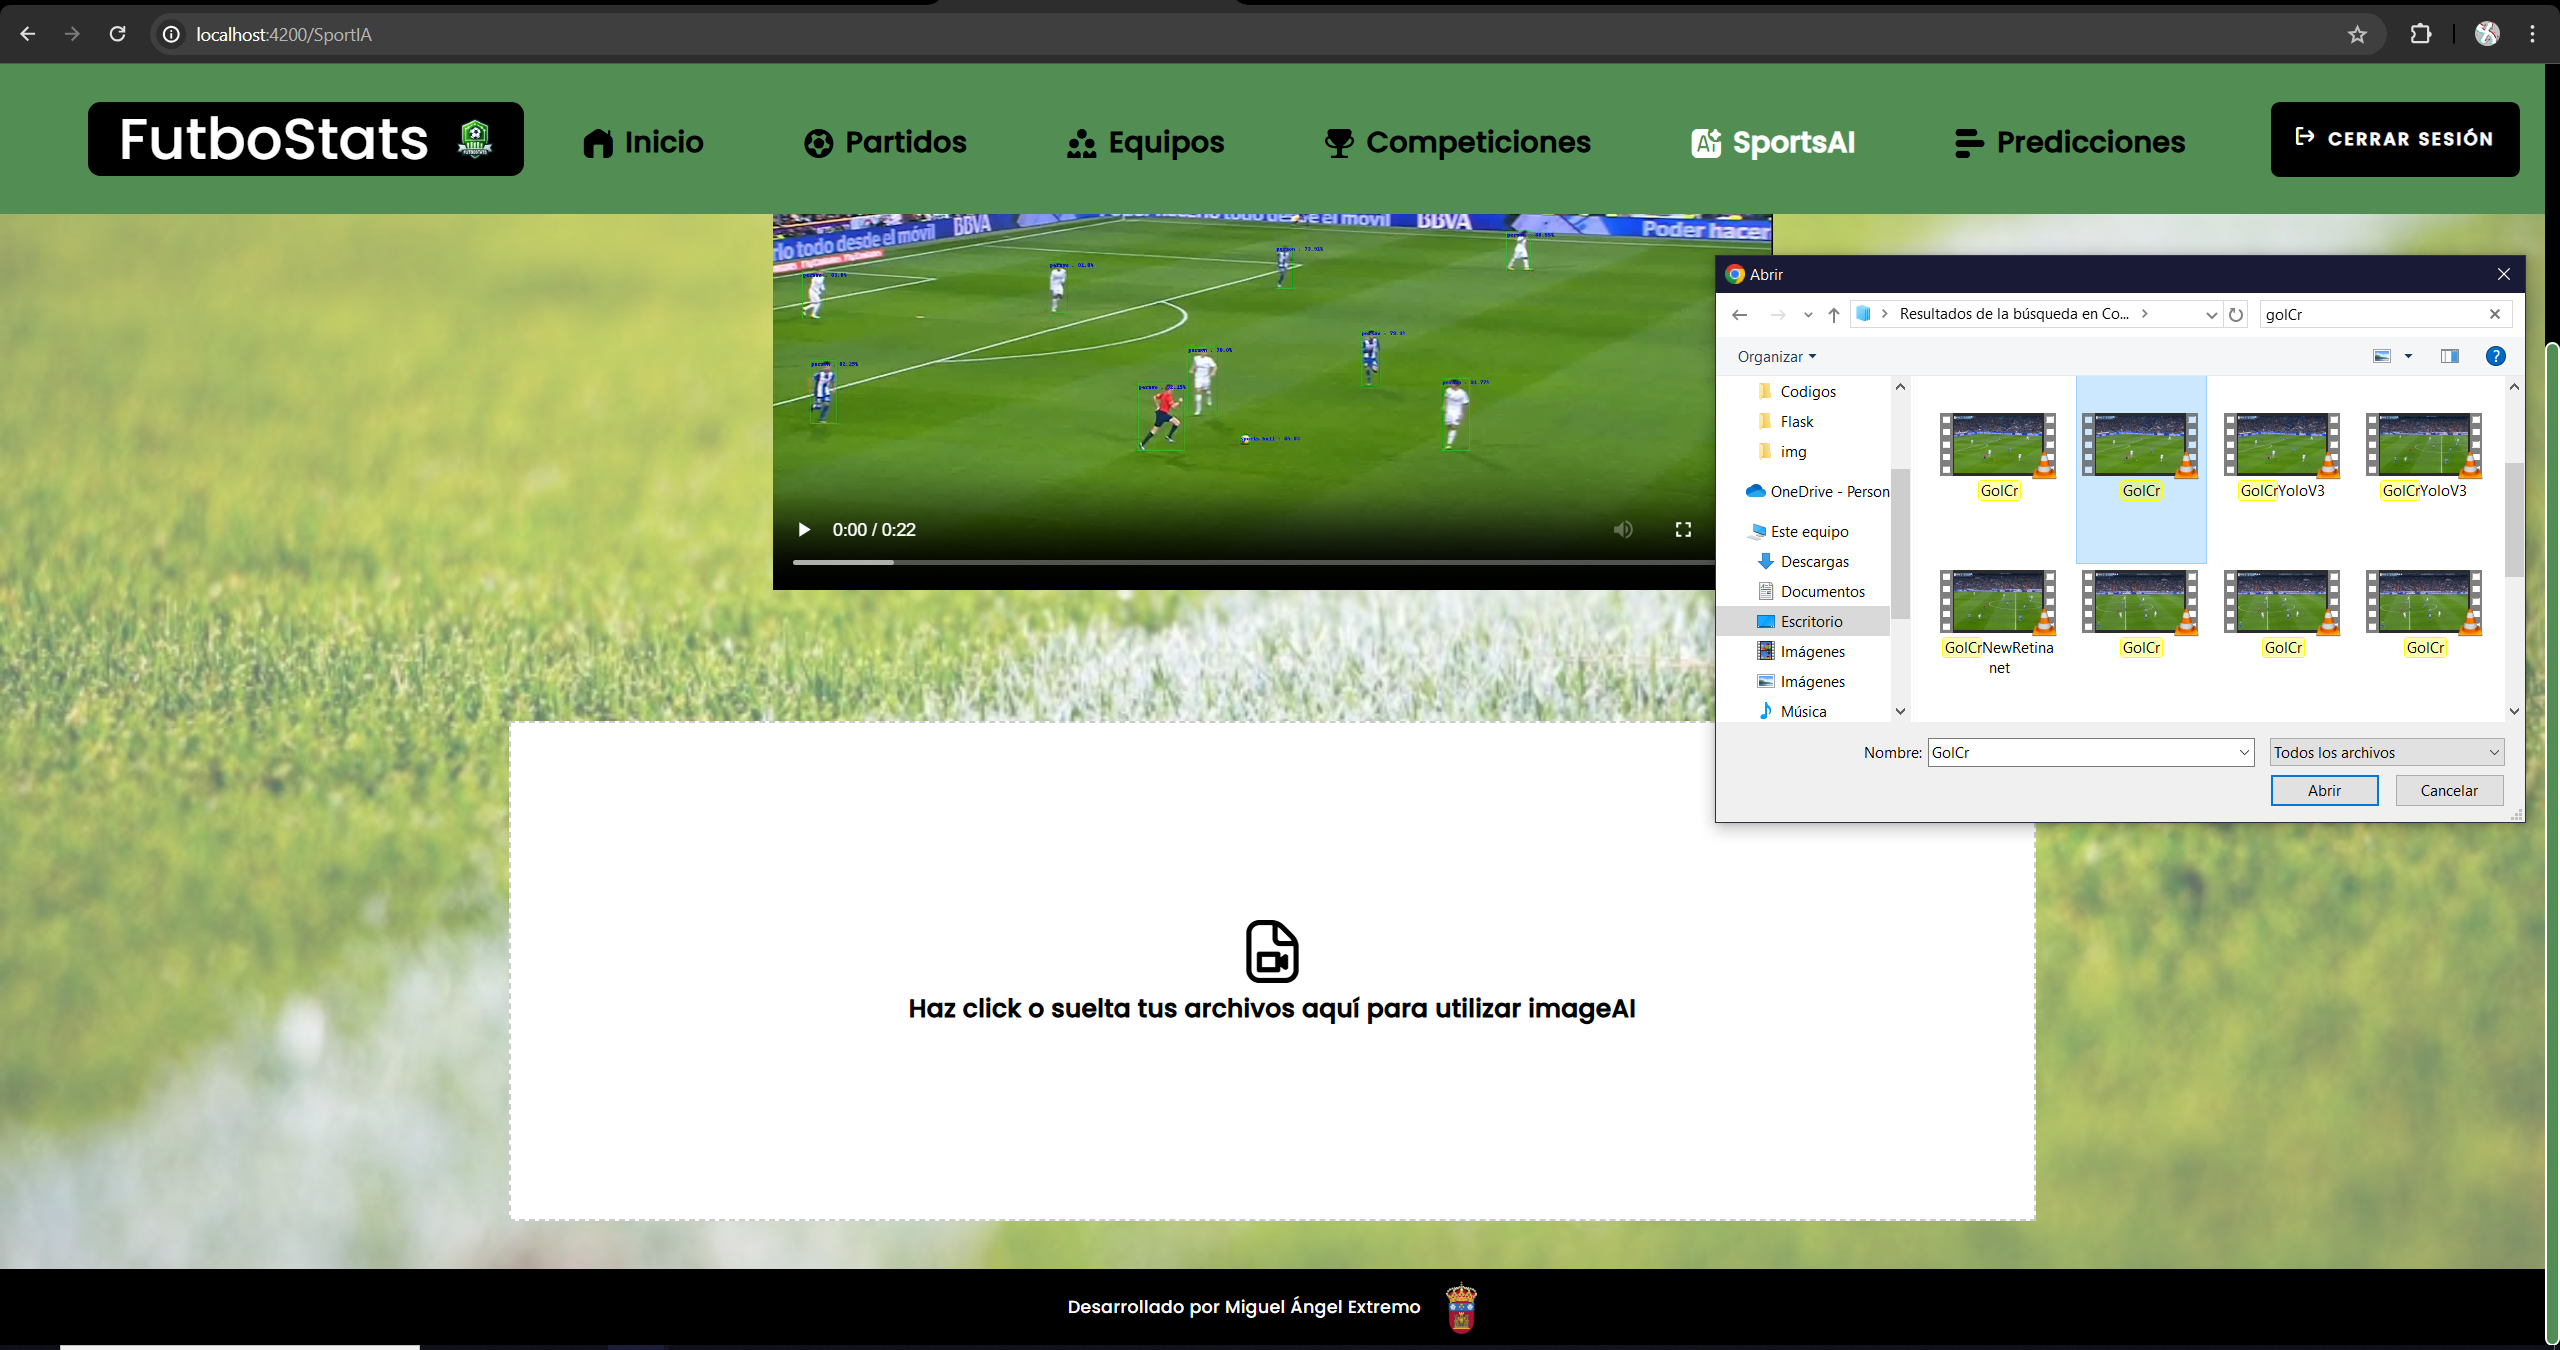
\includegraphics[width=1\linewidth]{img/sportsAI2-UM.png}
    \caption{Paso 2 para utilizar SportAI: pulsar o arrastrar un vídeo '.mp4'.}
    \label{fig:enter-label}
\end{figure}

\begin{figure}[H]
    \centering
    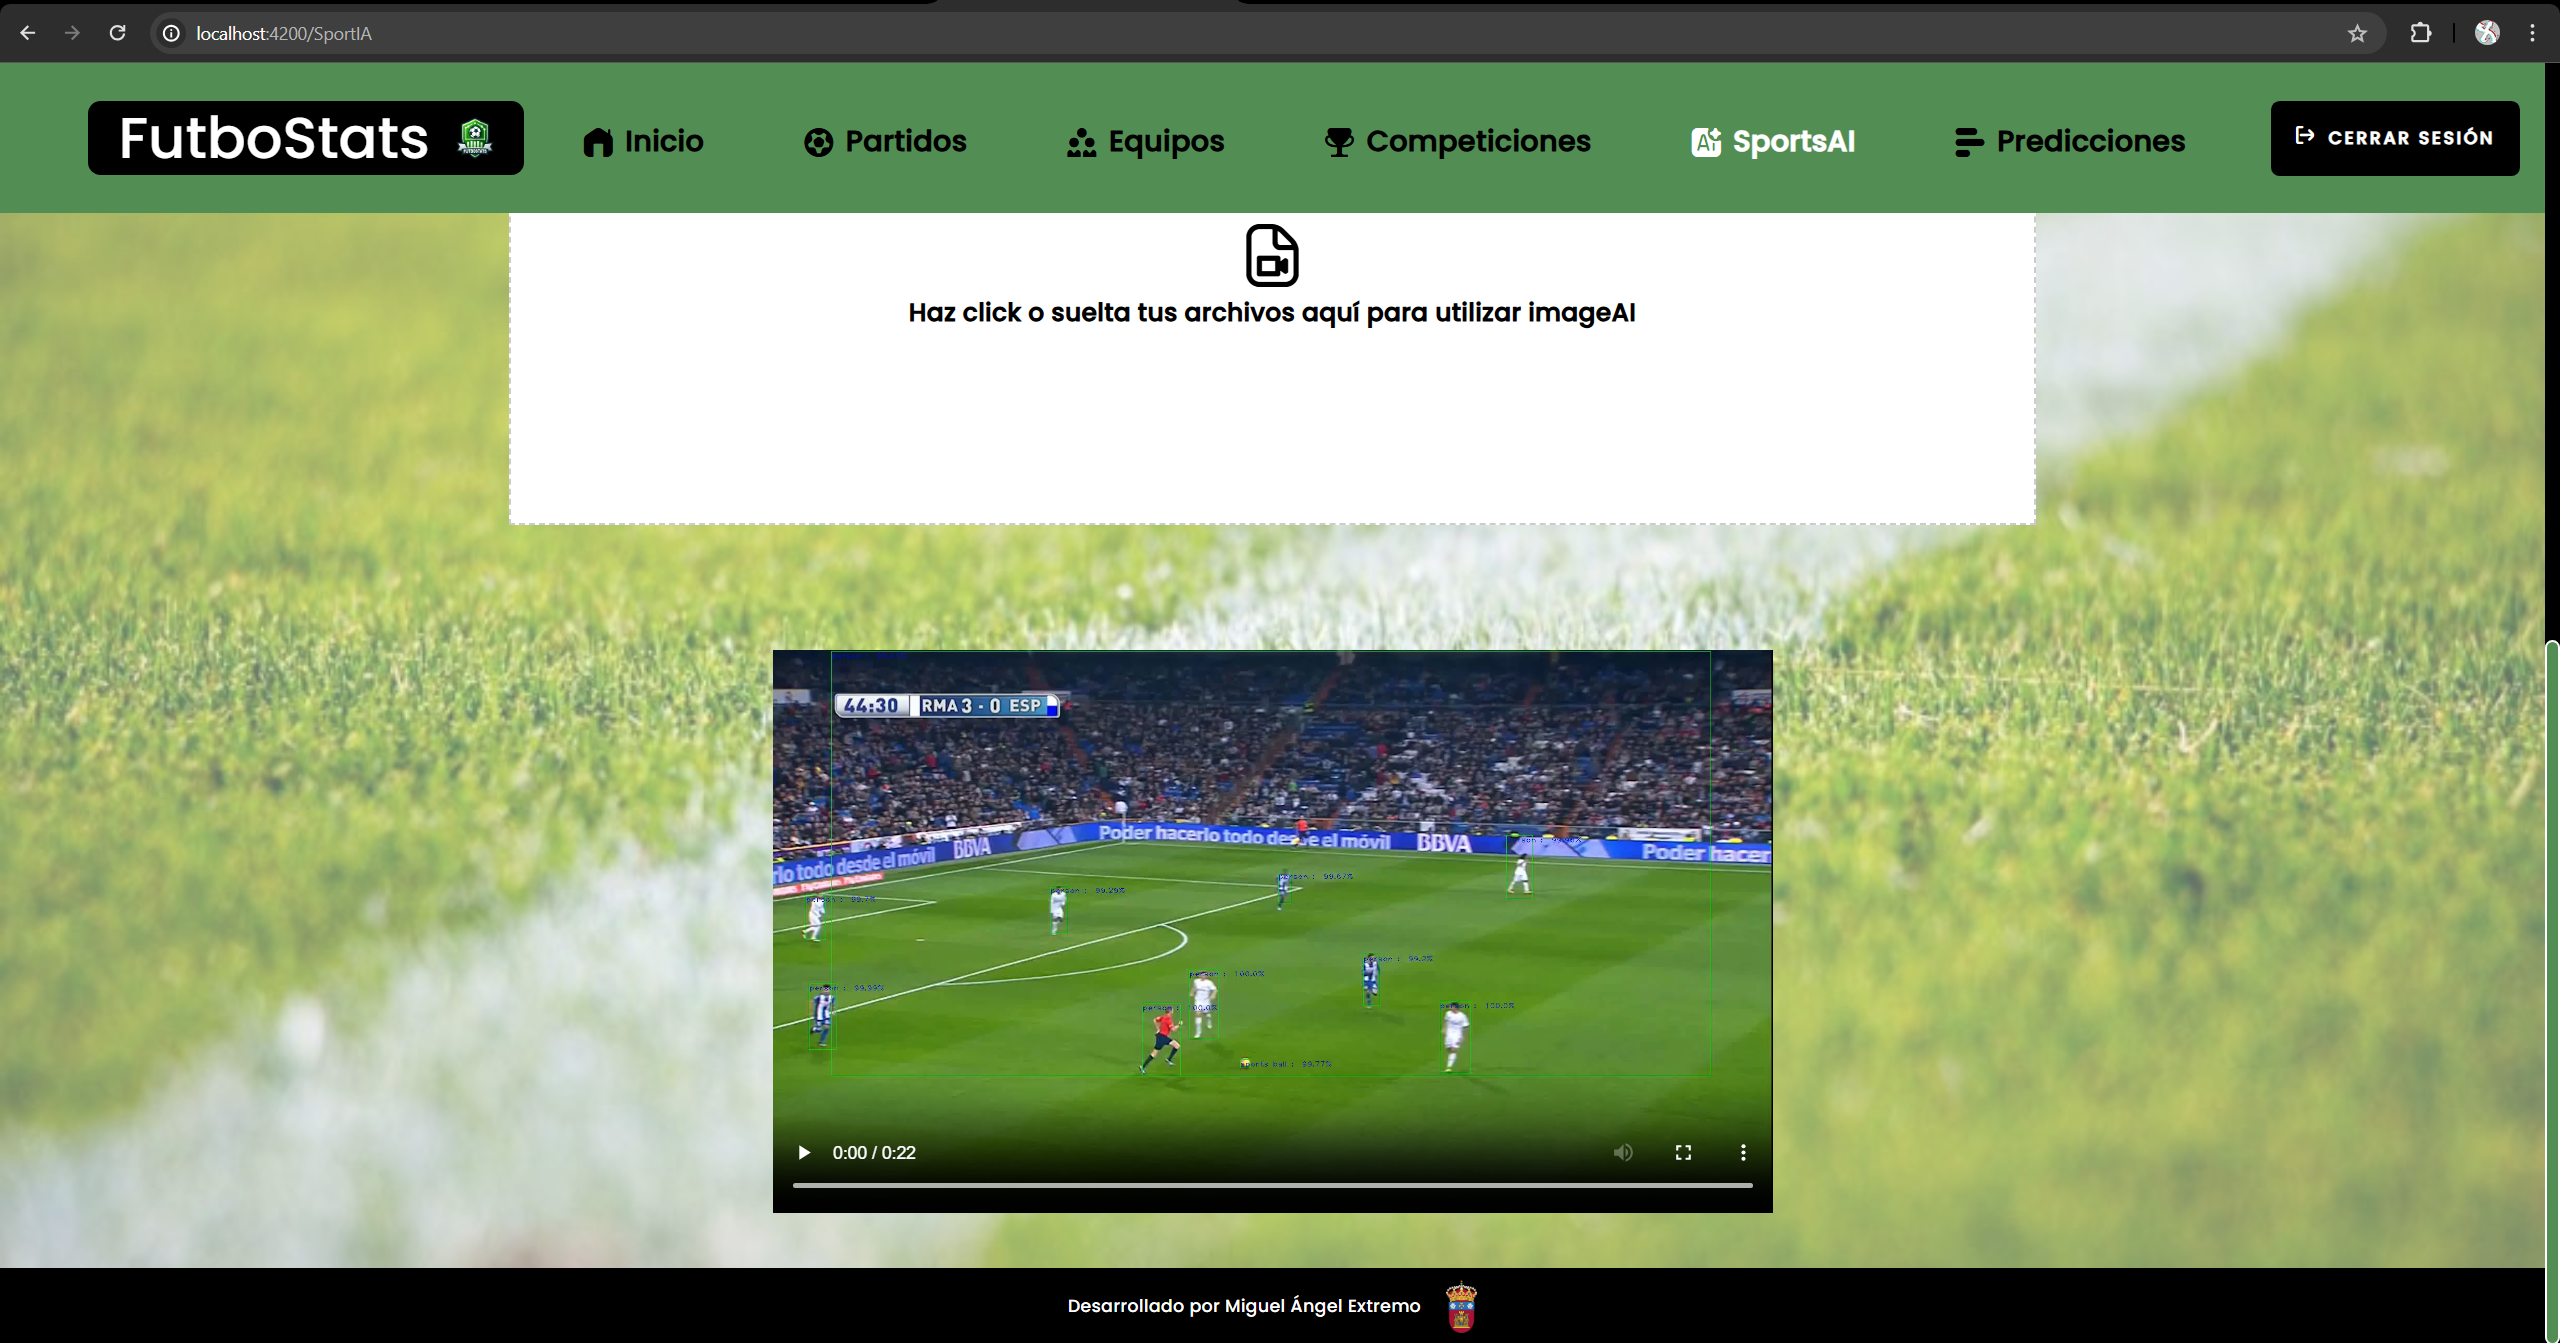
\includegraphics[width=1\linewidth]{img/sportsAI3-UM.png}
    \caption{Paso 3 para utilizar SportAI: visualizar el vídeo generado por imageAI}
    \label{fig:enter-label}
\end{figure}

\subsection{Utilizar Predicciones en FutboStats}
En la opción 'Predicciones' de FutboStats el usuario podrá consultar predicciones, modelo de goles esperados, puntos esperados y gráficas de estadísticas del mundial de una forma sencilla. \\
Los pasos a seguir son:
\begin{enumerate}
    \item Iniciar sesión en la aplicación.
    \item Pulsar en la opción 'Predicciones' del menú superior.
    \item El usuario accede a clasificaciones y puede visualizar una comparación entre la tabla de puntos esperados generada por el modelo y la clasificación real. Además, puede visualizar un gráfico que muestra el desarrollo de los equipos en la liga a lo largo de las jornadas. Las ligas disponibles son La Liga, Bundesliga, Premier League, Serie A y Ligue1. Los datos pertenecen a la temporada 2015/2016.
    \item El usuario puede pulsar en el menú secundario y acceder a 'Goles esperados xG'. El usuario puede visualizar los resultados del modelo mediante tablas y gráficas. Si el usuario hace click o pone el cursor encima de las tarjetas podrá leer información acerca de las representaciones gráficas.
    \item El usuario puede pulsar en el menú secundario y accedera 'Mundial'. El usuario puede visualizar gráficos que representan estadísticas de la final del mundial de 2022 entre Francia y Argentina. El usuario puede elegir el gráfico que quiere visualizar eligiendo el jugador que prefiera. Si el usuario hace click o pone el cursor encima de la tarjeta podrá leer información acerca de las representaciones gráficas.
\end{enumerate}

\begin{figure}[H]
    \centering
    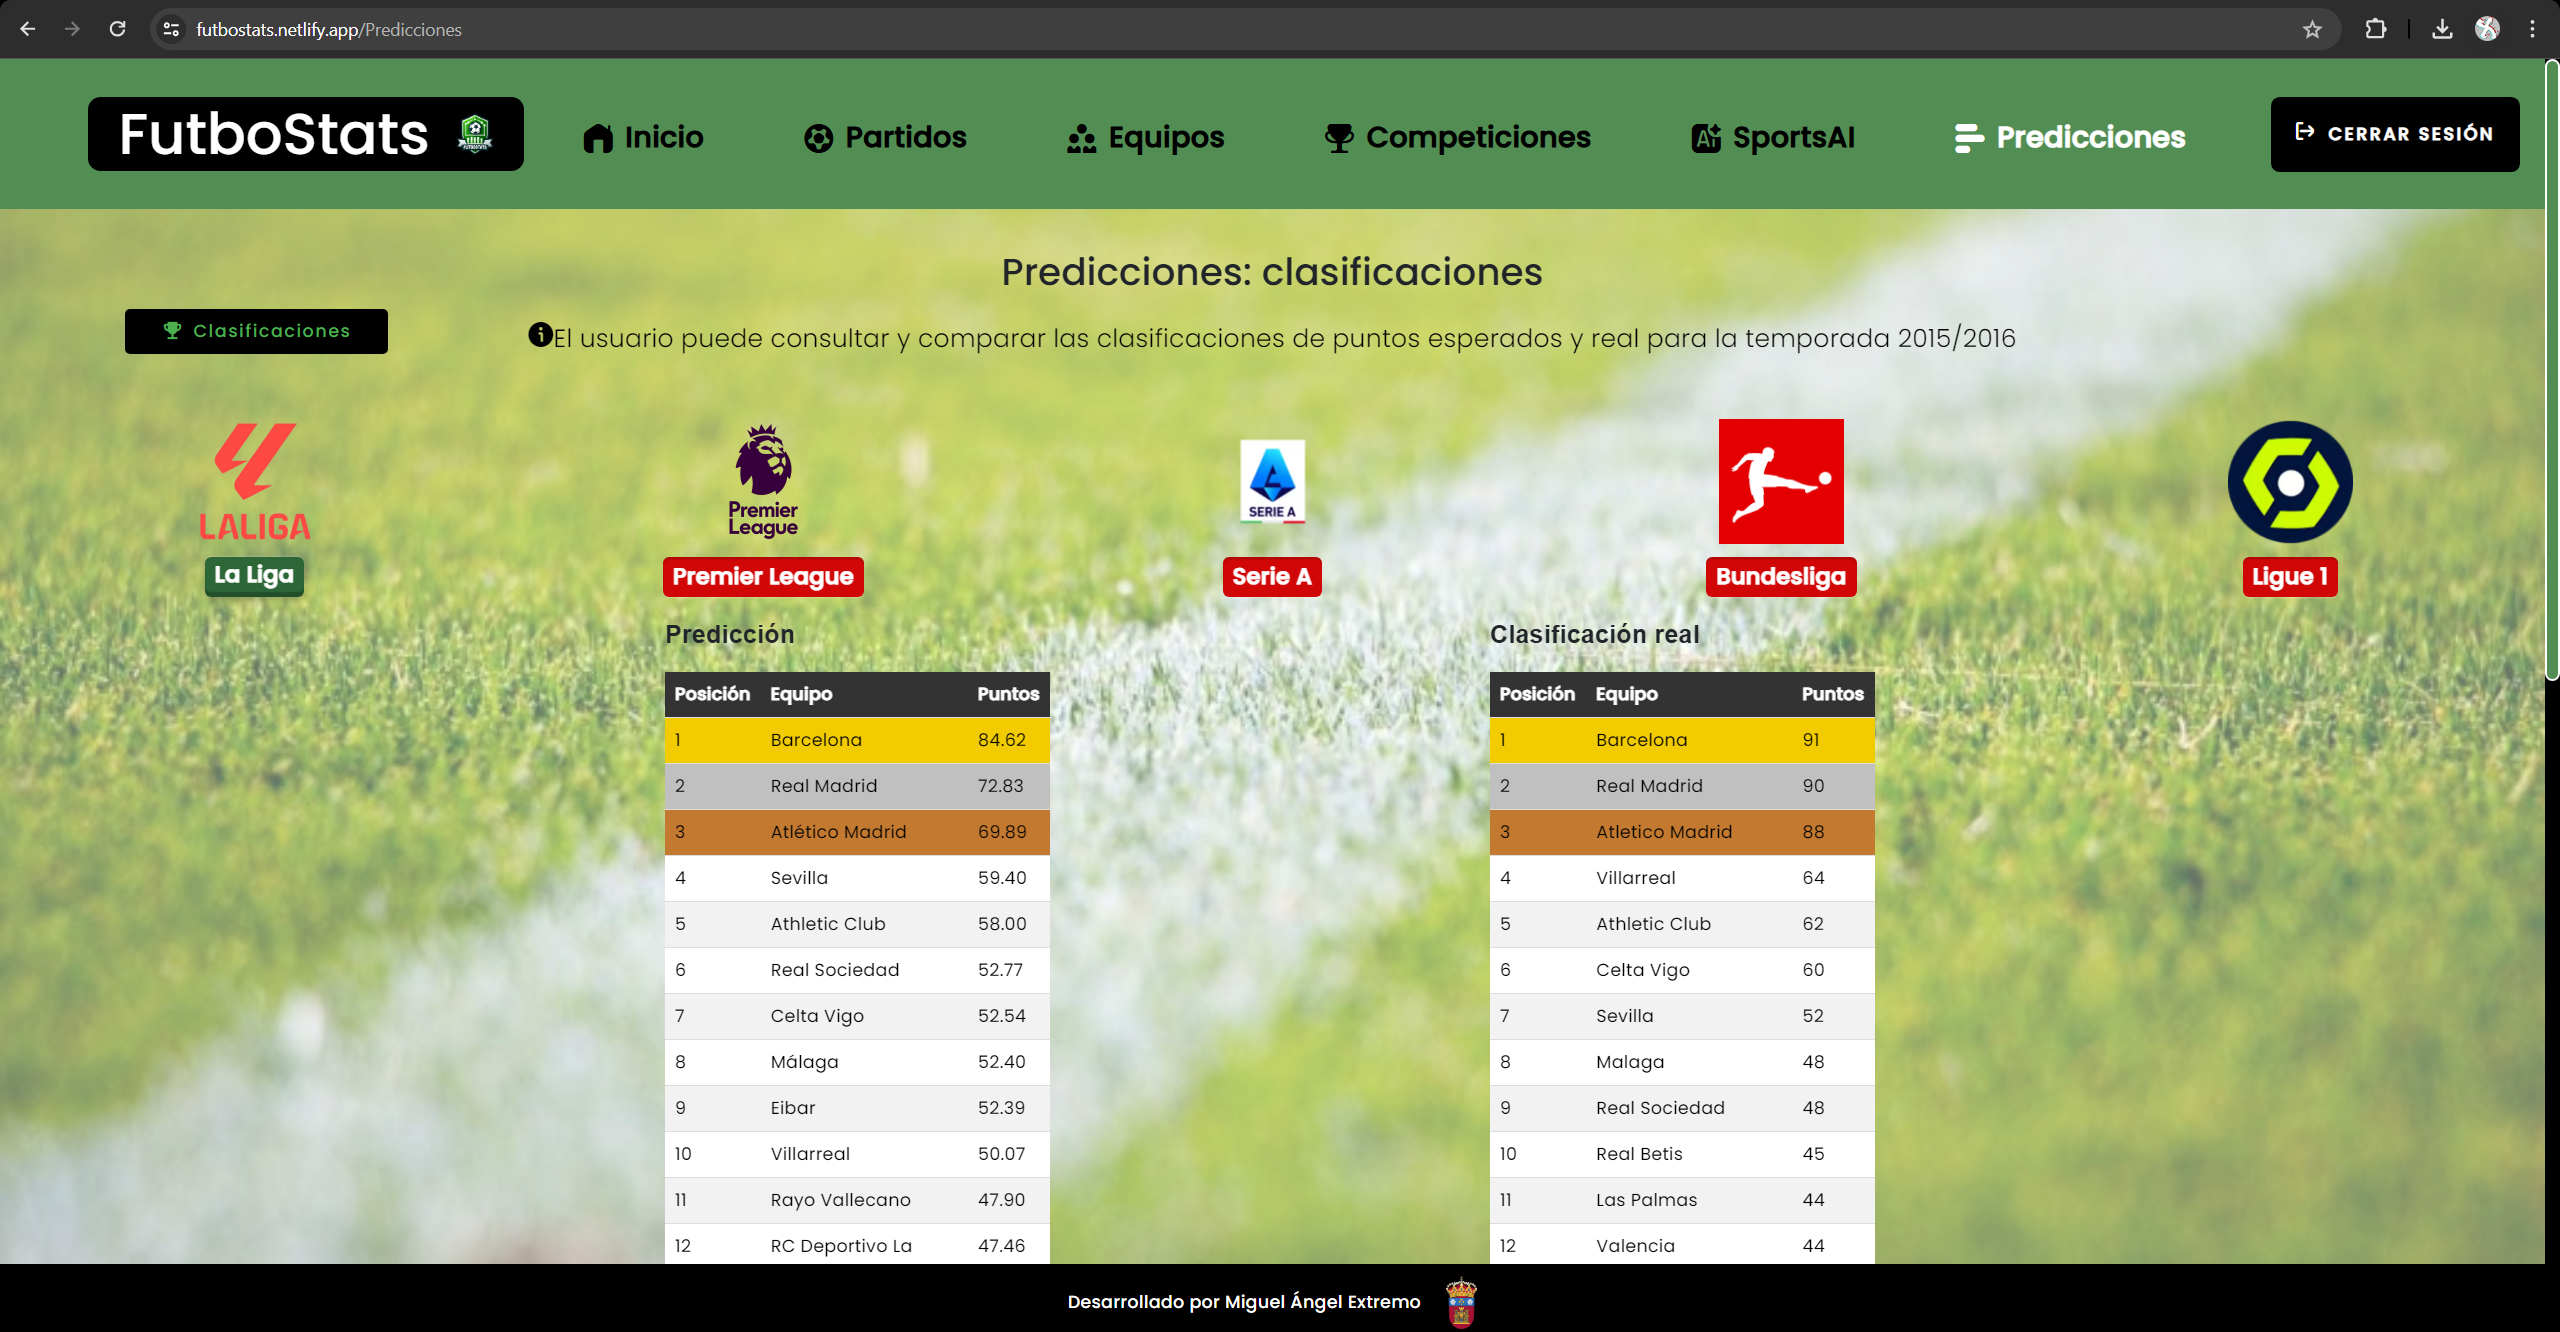
\includegraphics[width=1\linewidth]{img/predicciones1-UM.png}
    \caption{Visualización de predicción de puntos esperados y real.}
    \label{fig:enter-label}
\end{figure}

\begin{figure}[H]
    \centering
    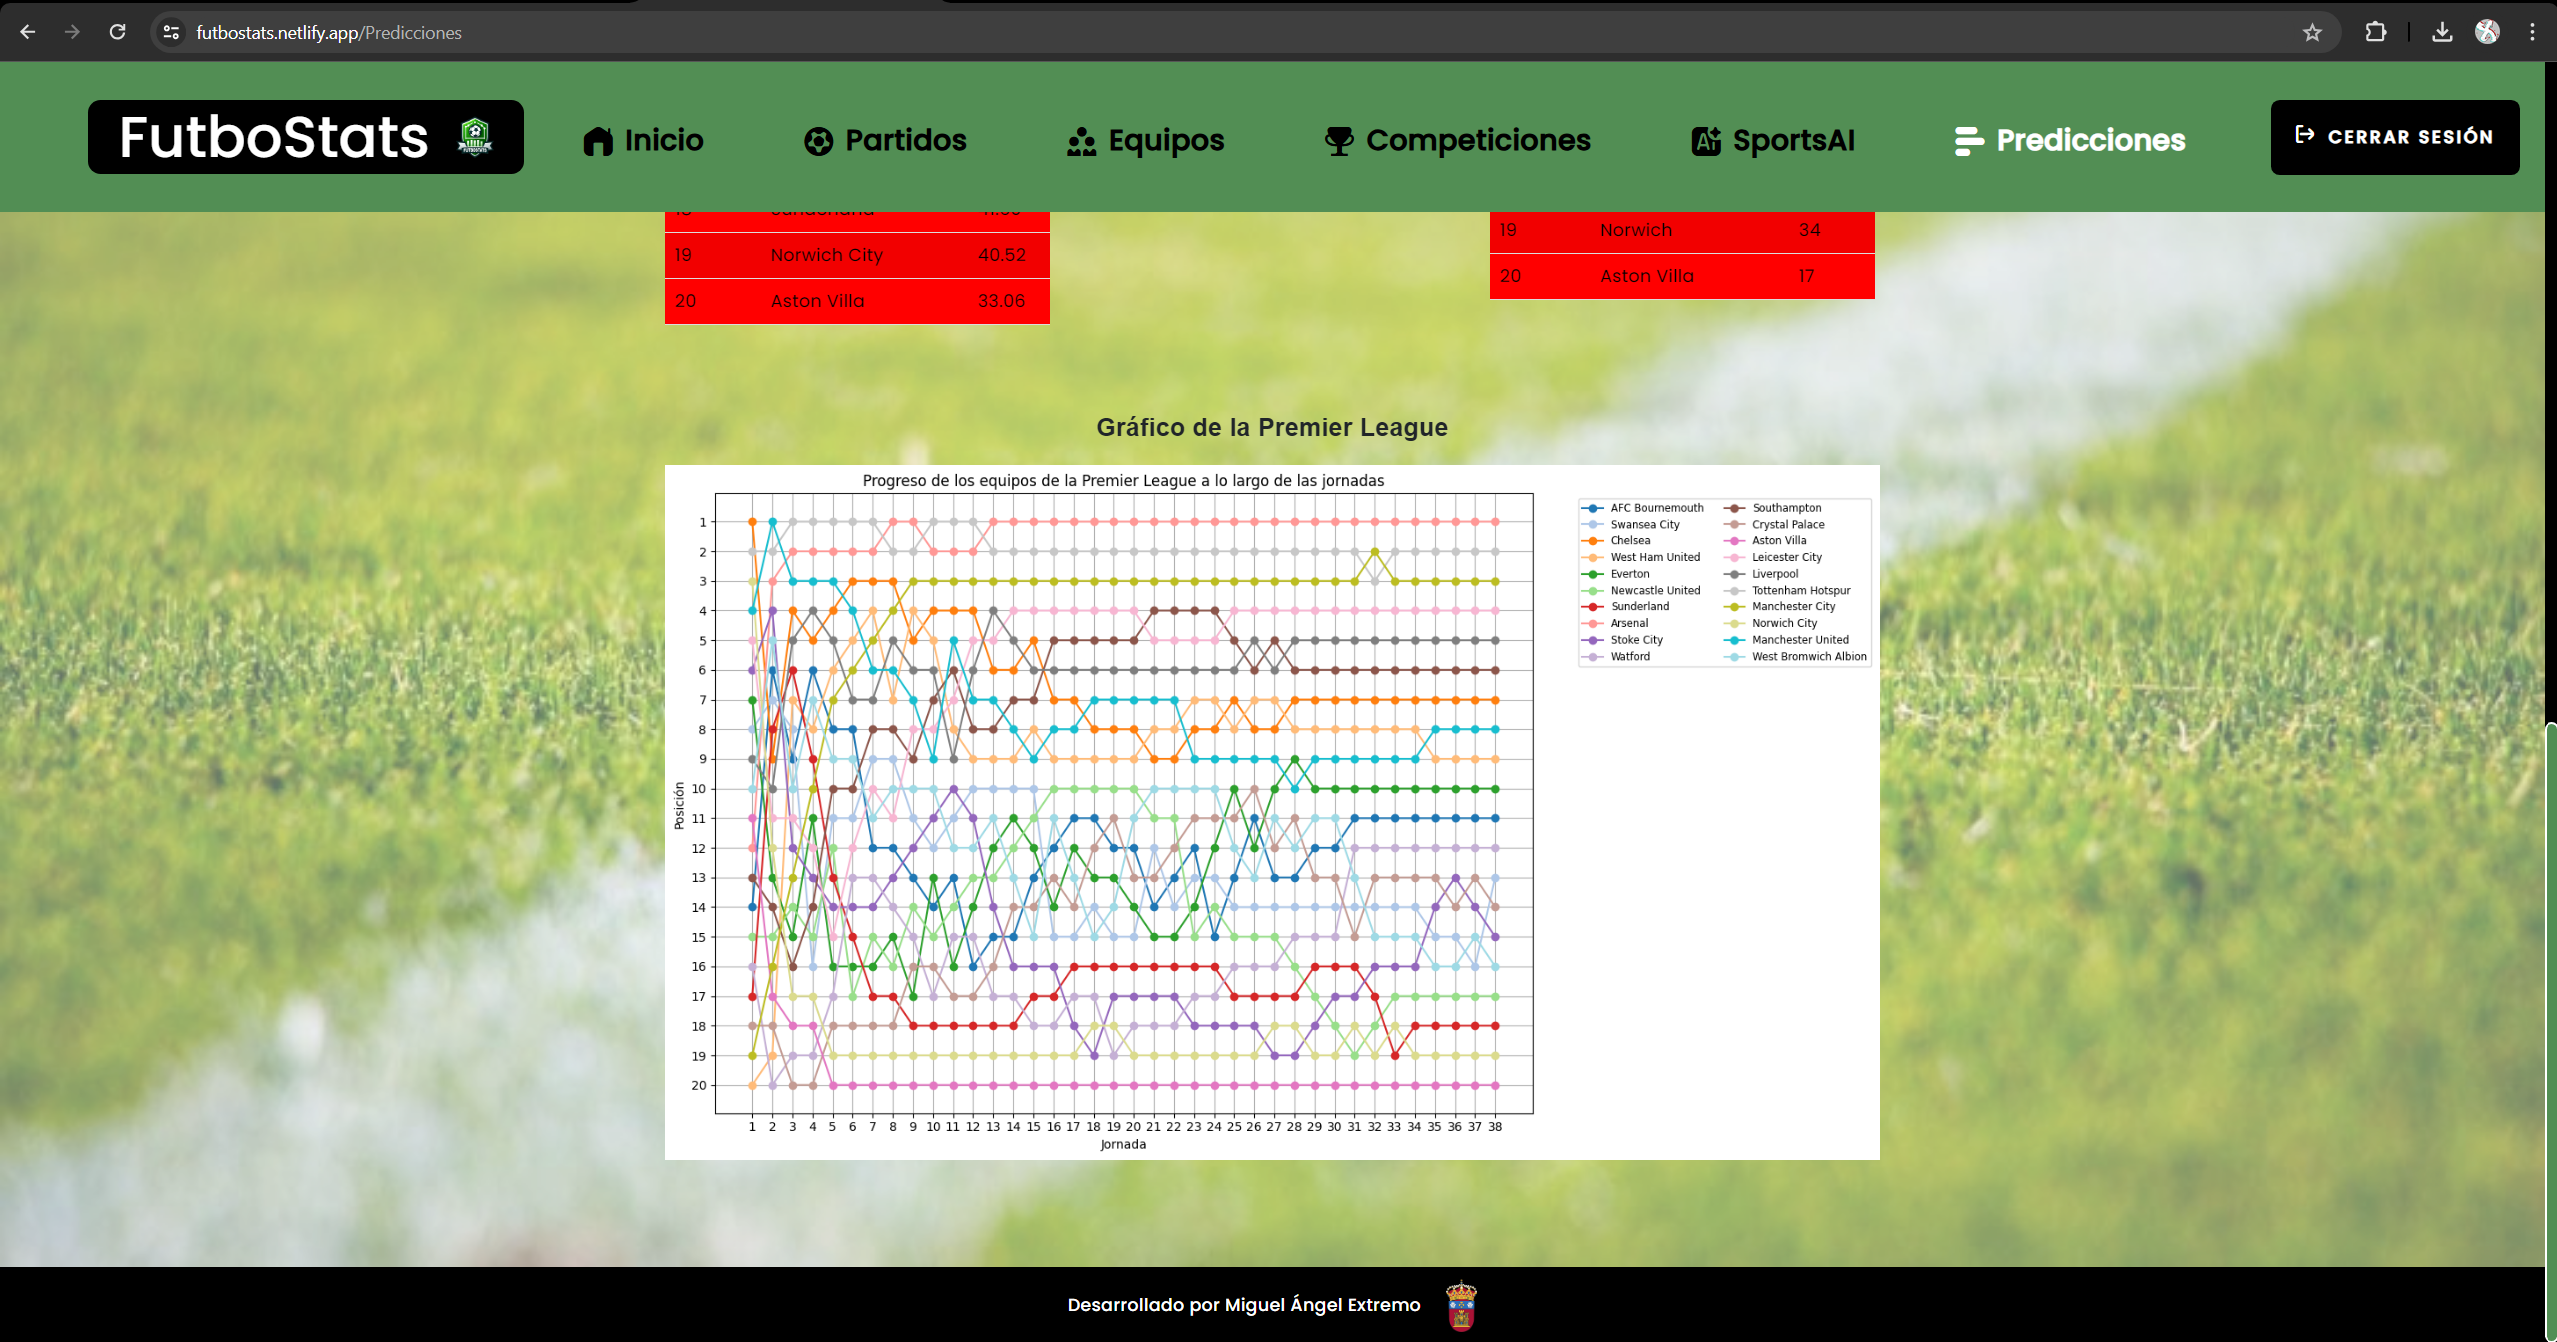
\includegraphics[width=1\linewidth]{img/predicciones2-UM.png}
    \caption{Representación gráfica de los puntos esperados a lo largo de las jornadas.}
    \label{fig:enter-label}
\end{figure}

\begin{figure}[H]
    \centering
    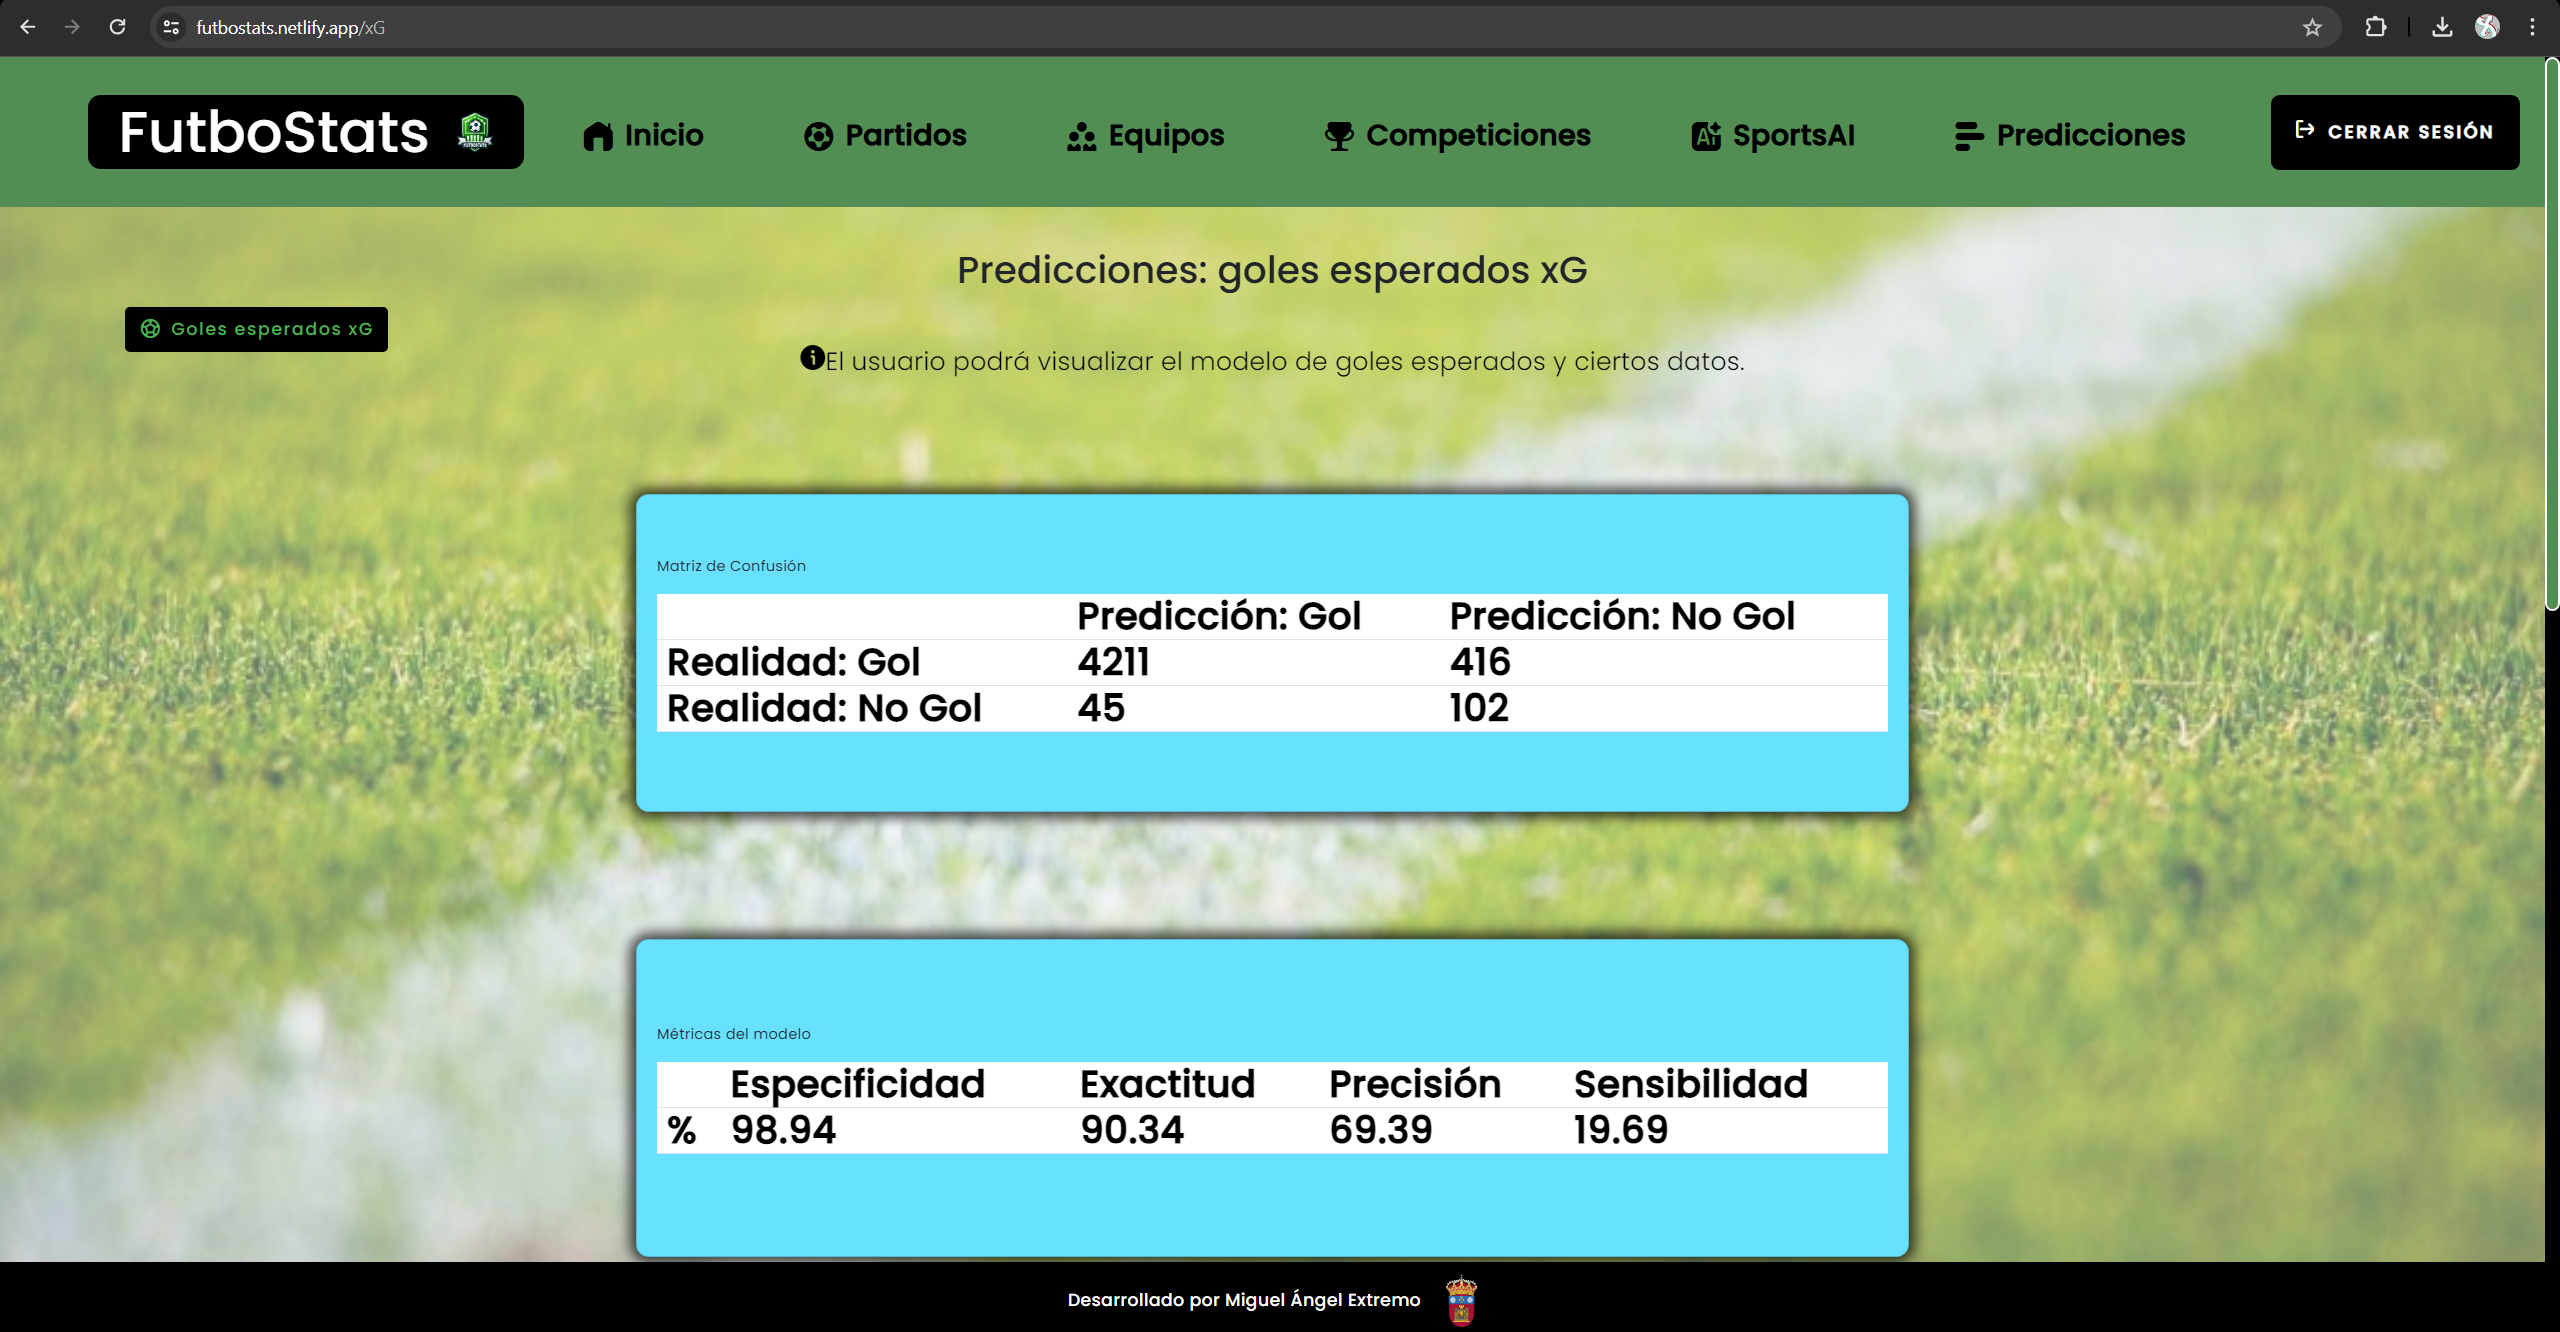
\includegraphics[width=1\linewidth]{img/golesEsperados1-UM.png}
    \caption{Visualización tablas del modelo de goles esperados xG}
    \label{fig:enter-label}
\end{figure}

\begin{figure}[H]
    \centering
    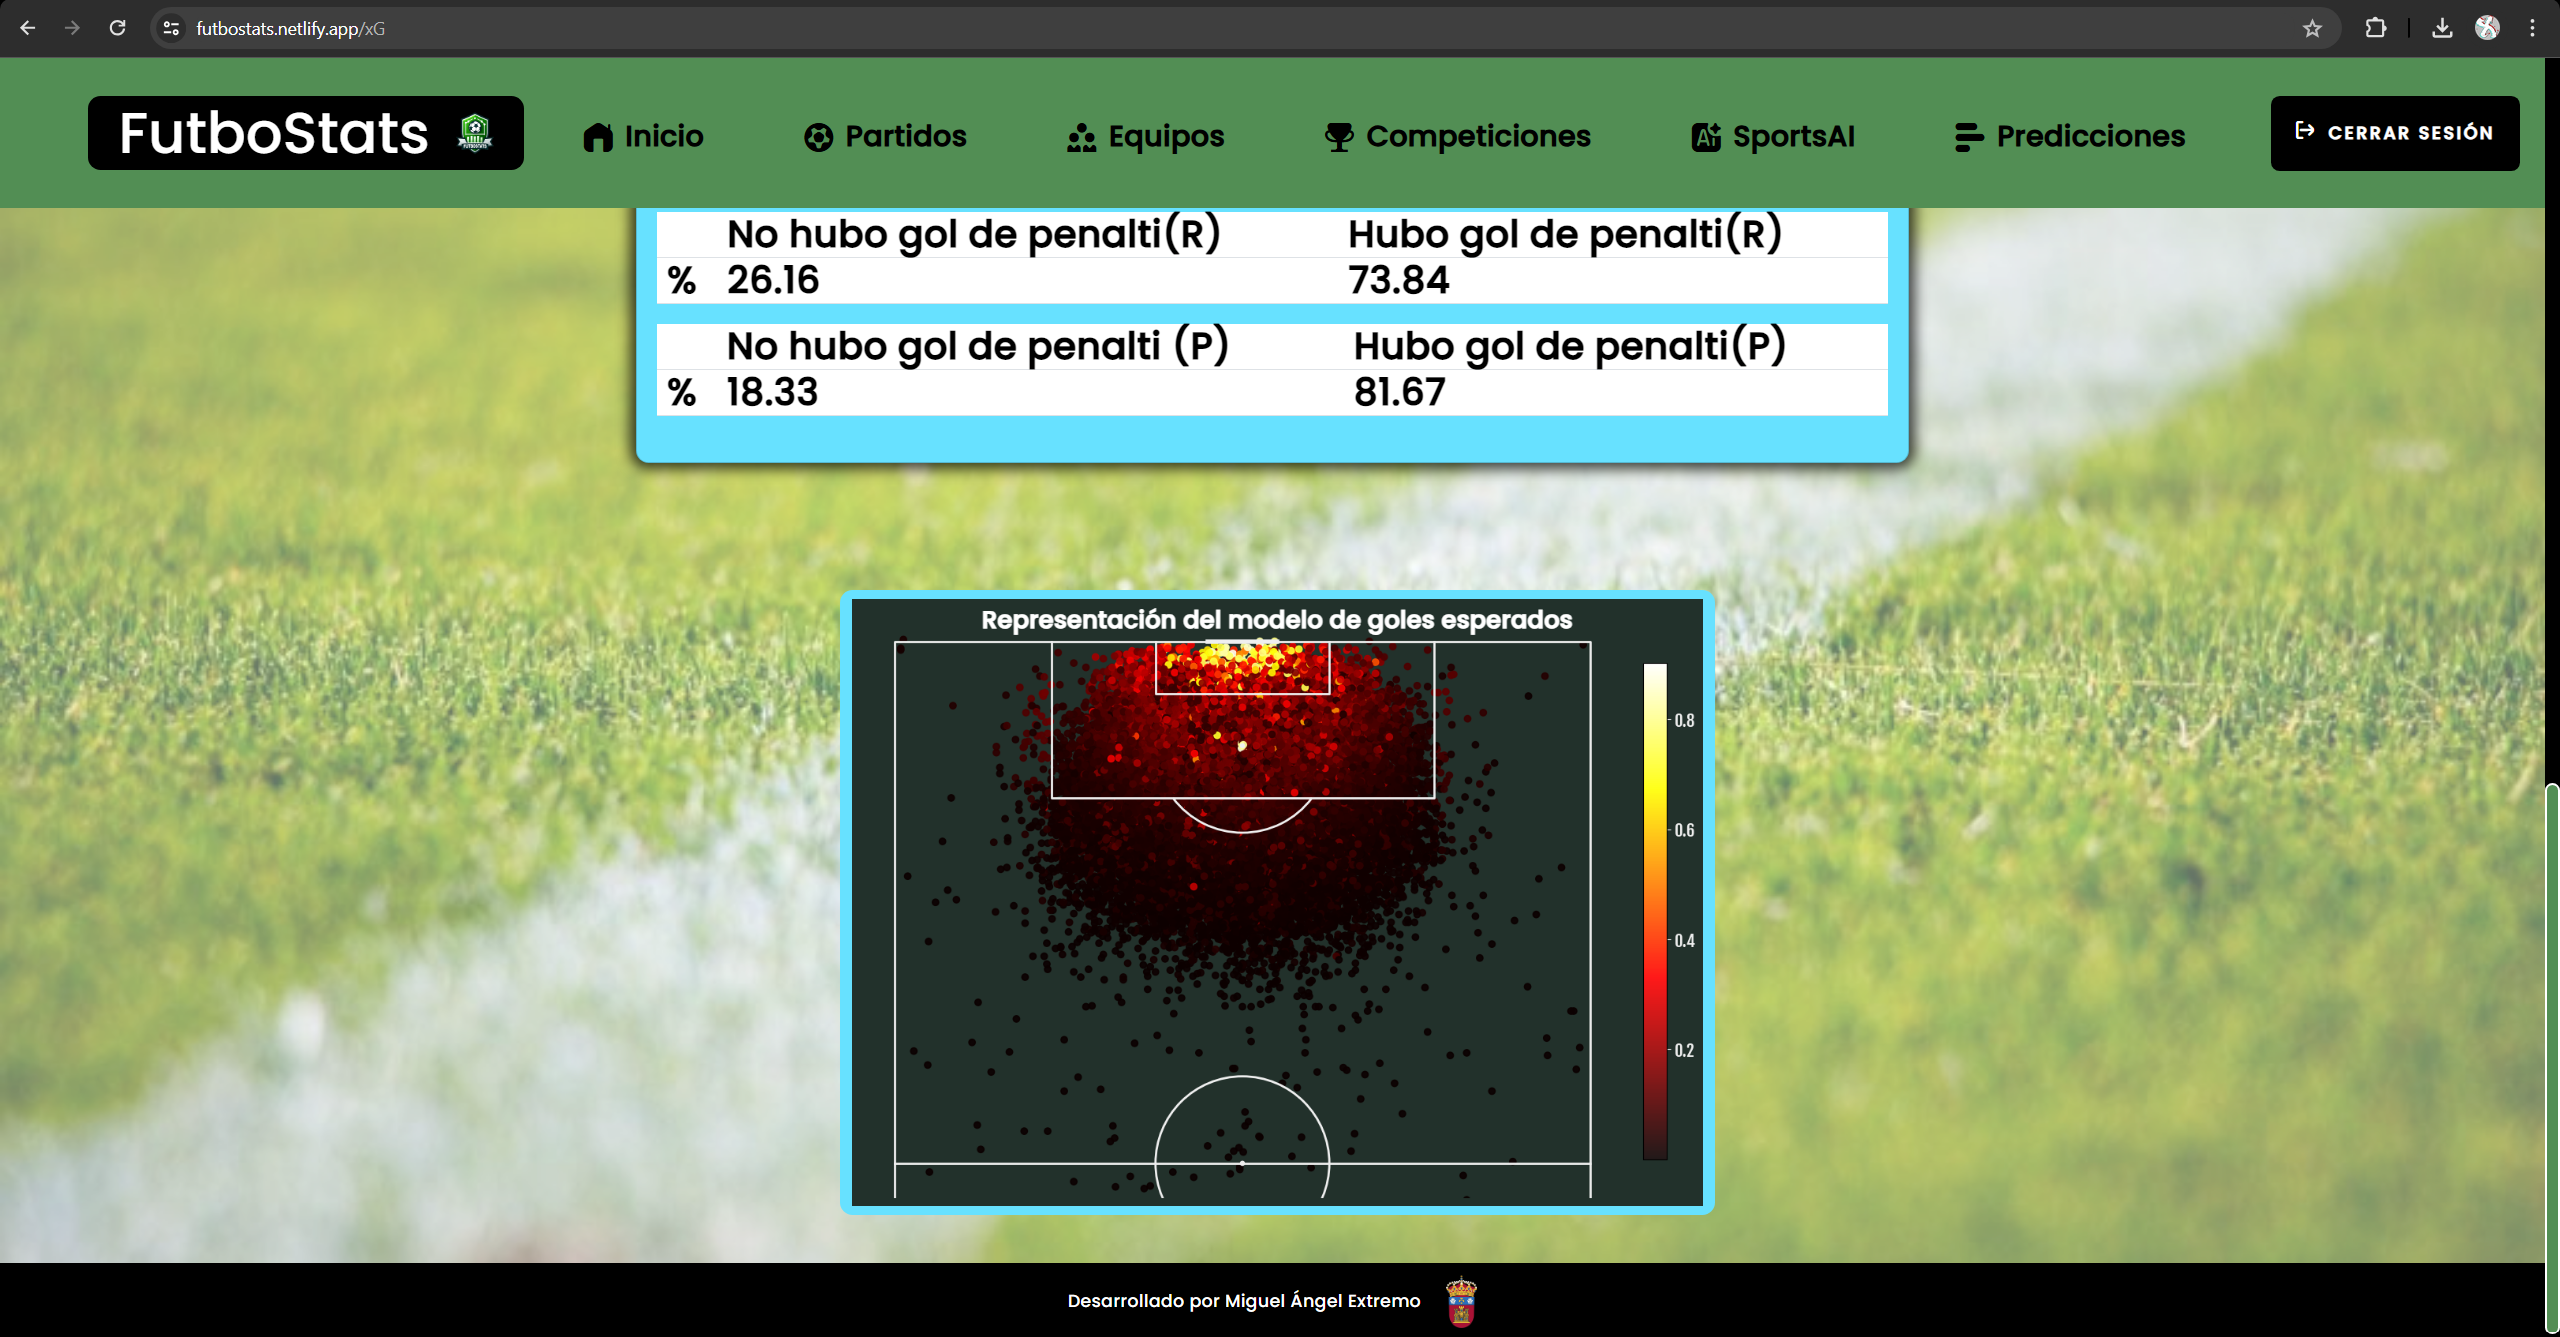
\includegraphics[width=1\linewidth]{img/golesEsperados2-UM.png}
    \caption{Representación gráfica del modelo de goles esperados xG.}
    \label{fig:enter-label}
\end{figure}

\begin{figure}[H]
    \centering
    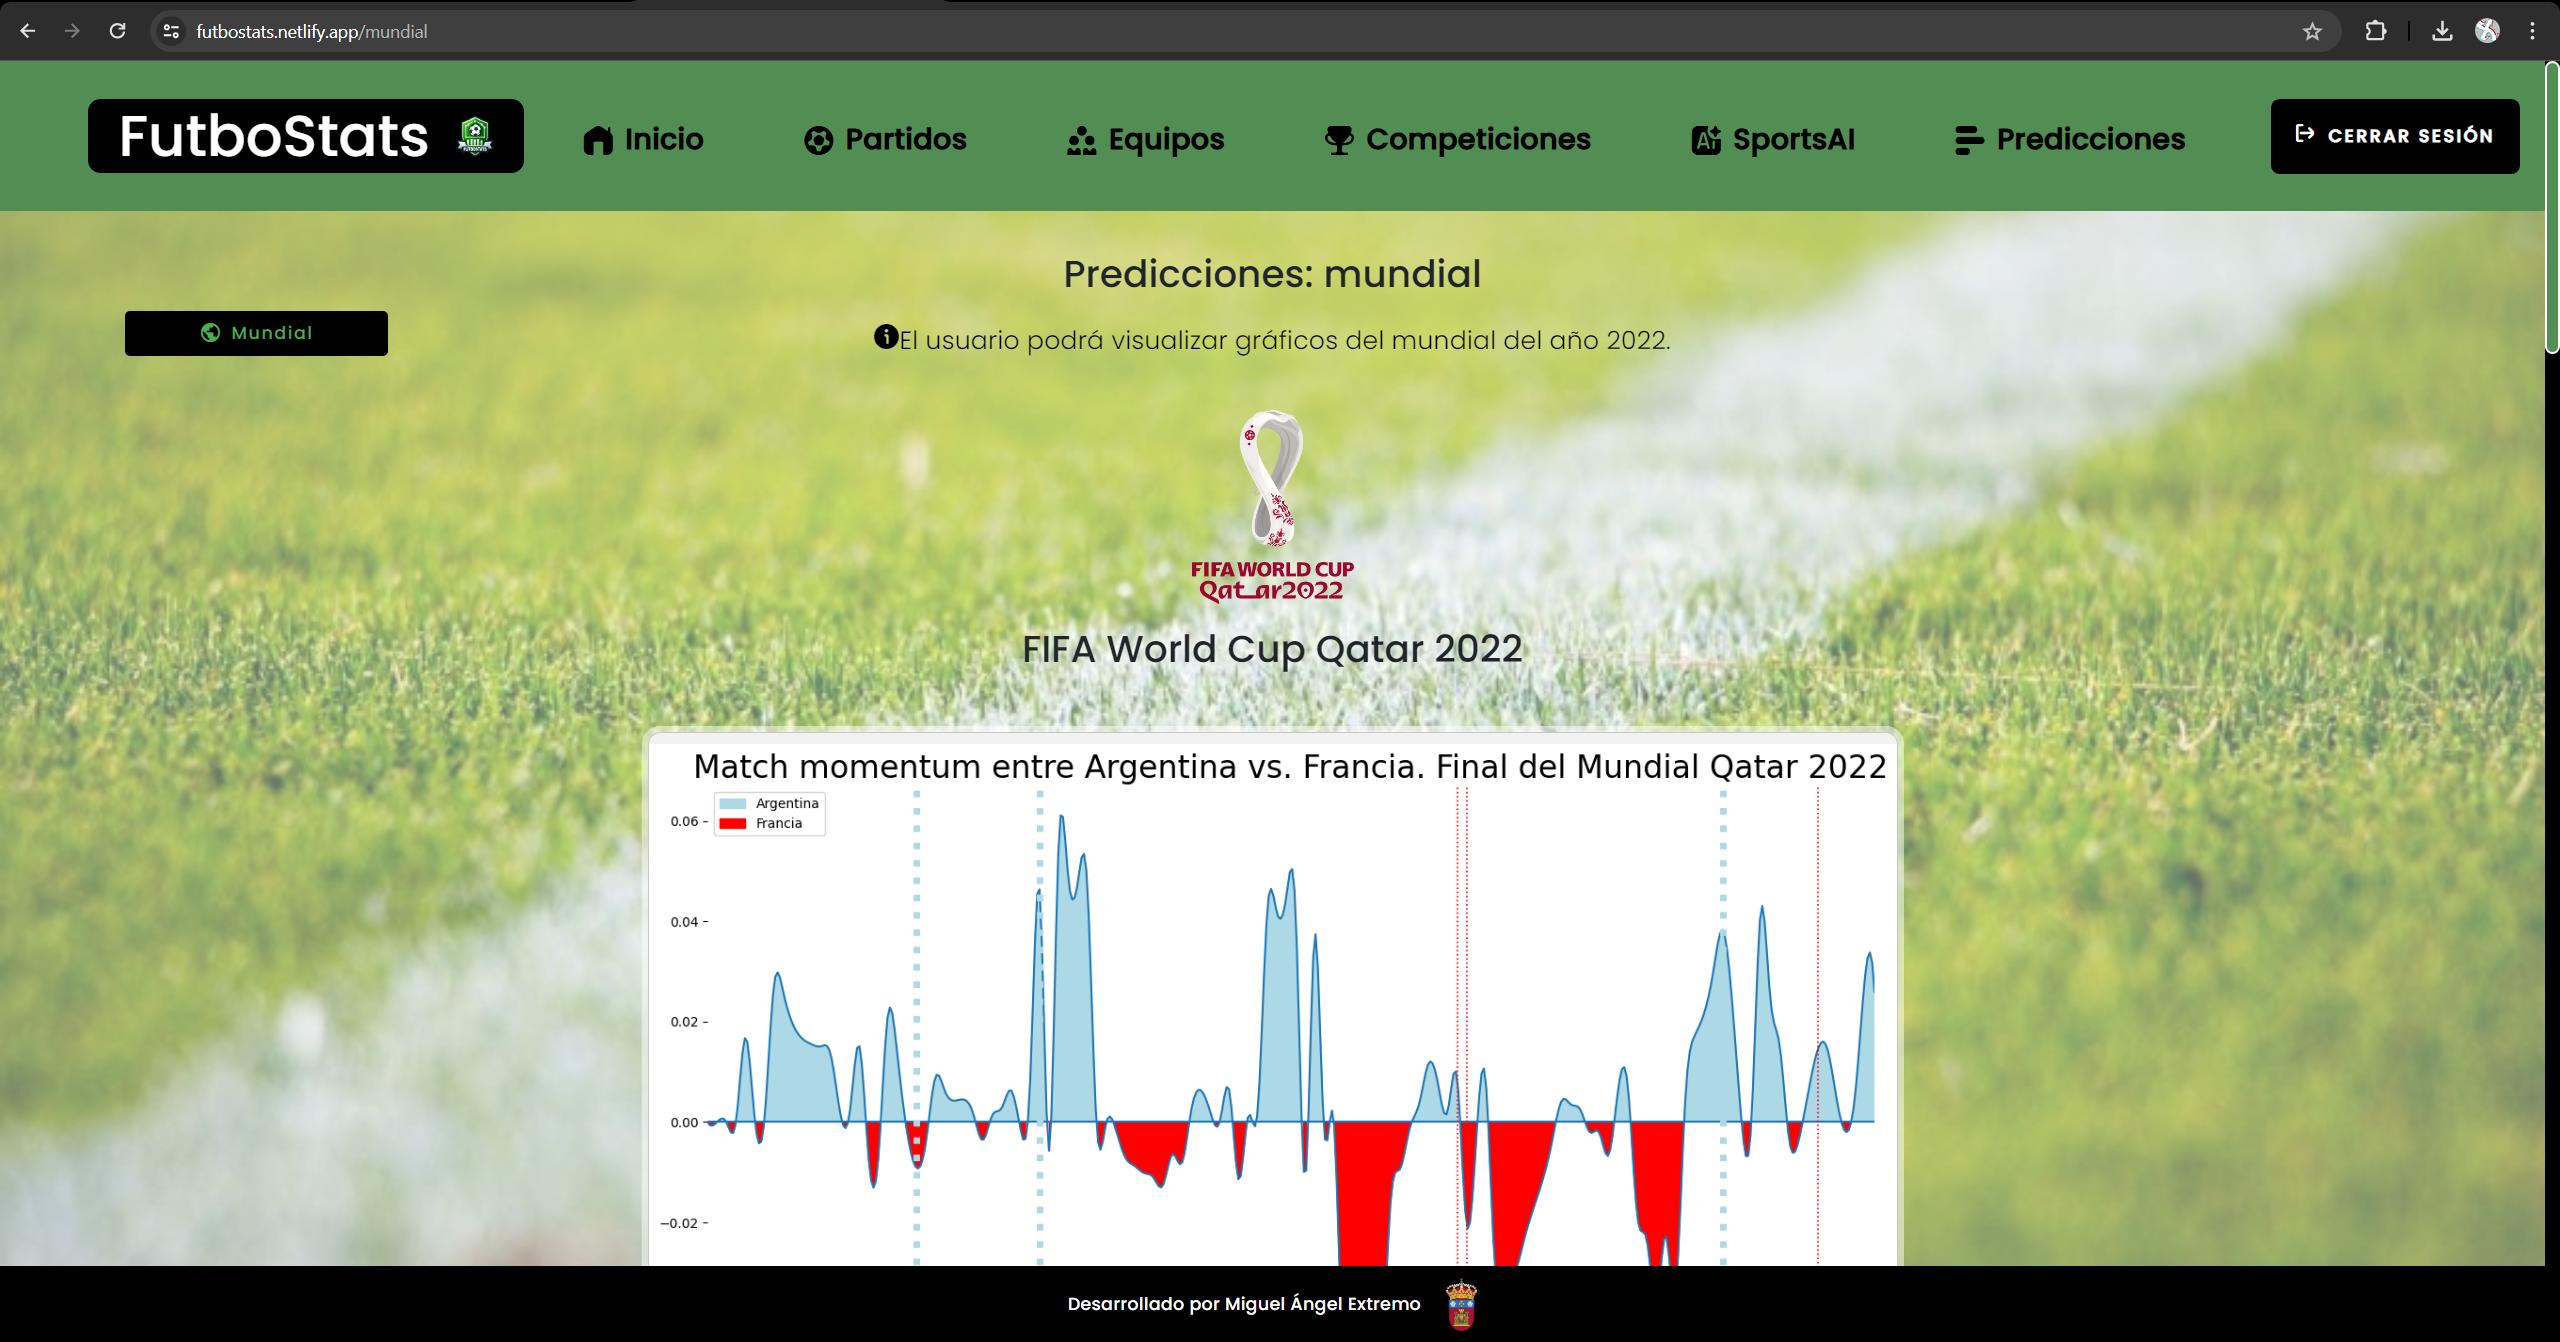
\includegraphics[width=1\linewidth]{img/mundial1-UM.png}
    \caption{Visualización de las estadísticas del mundial 2022}
    \label{fig:enter-label}
\end{figure}

\begin{figure}[H]
    \centering
    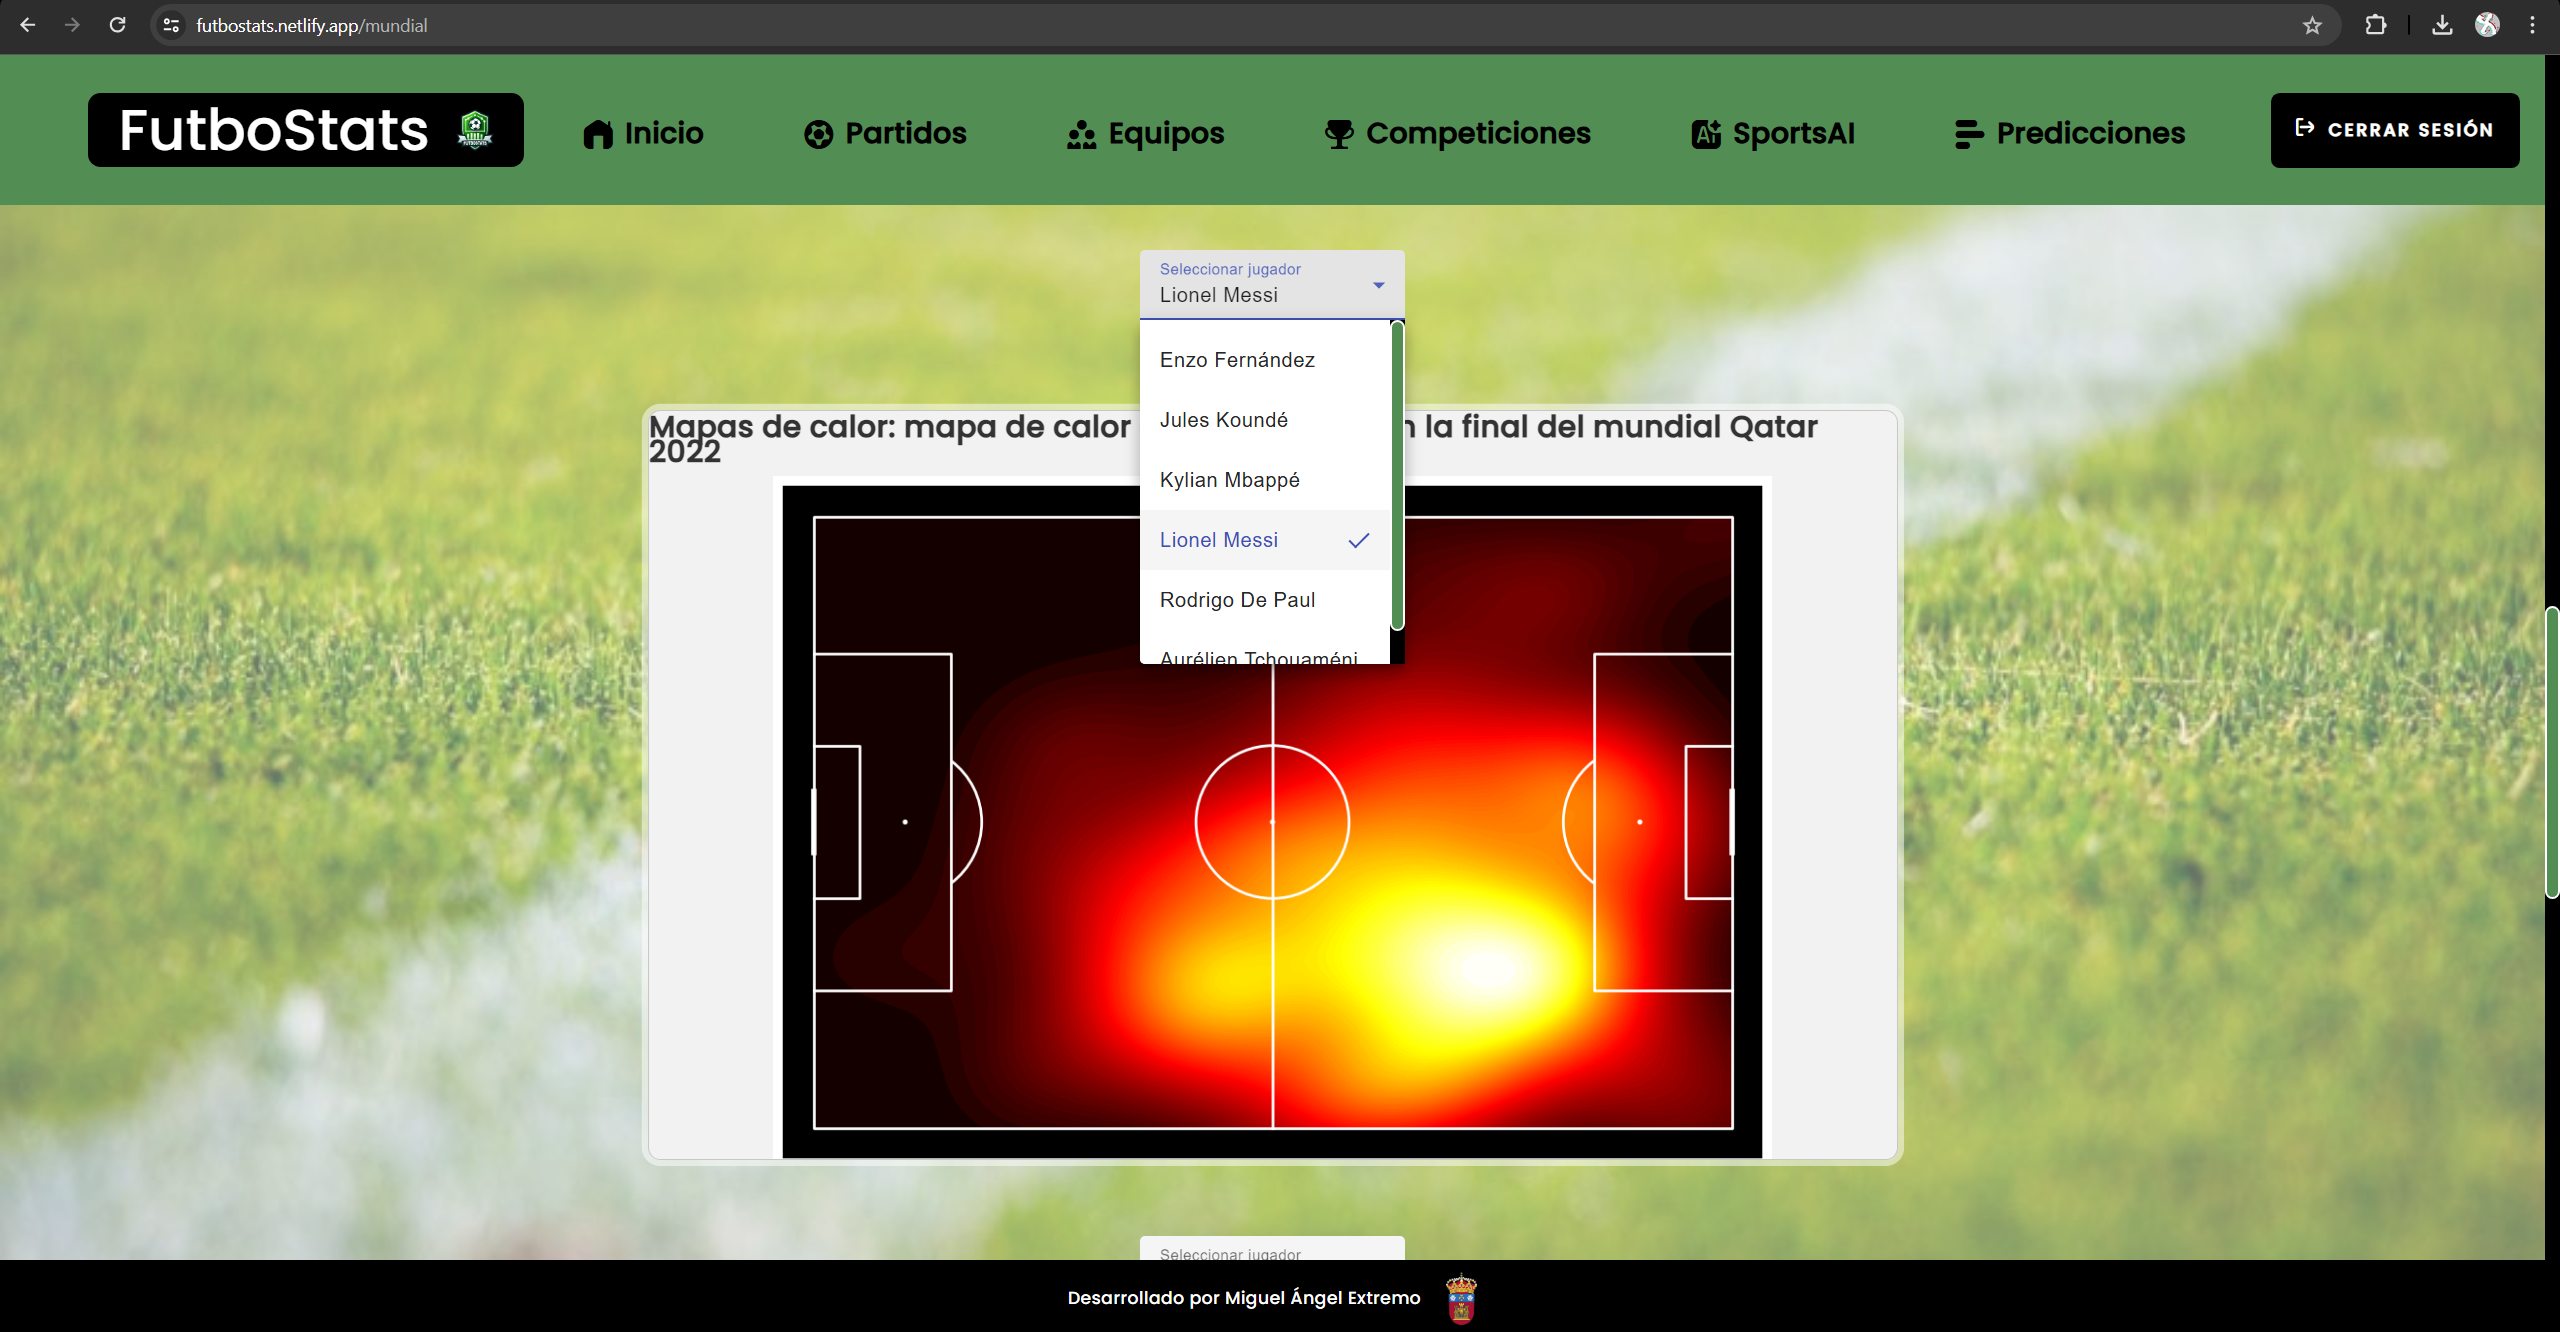
\includegraphics[width=1\linewidth]{img/mundial2-UM.png}
    \caption{Seleccionar el jugador para visualizar su gráfico.}
    \label{fig:enter-label}
\end{figure}


\apendice{Anexo de sostenibilización curricular}

\section{Introducción}
Este anexo incluirá una reflexión personal del alumnado sobre los aspectos de la sostenibilidad que se abordan en el trabajo.
Se pueden incluir tantas subsecciones como sean necesarias con la intención de explicar las competencias de sostenibilidad adquiridas durante el alumnado y aplicadas al Trabajo de Fin de Grado.

Más información en el documento de la CRUE \url{https://www.crue.org/wp-content/uploads/2020/02/Directrices_Sosteniblidad_Crue2012.pdf}.

Este anexo tendrá una extensión comprendida entre 600 y 800 palabras.



\bibliographystyle{plain}
\bibliography{bibliografiaAnexos}

\end{document}
